\documentclass[oneside]{utmthesis}
%By default, print on two-side, can change to oneside printing 
%According to the new manual, should not mixed single-side with two-side printing

\usepackage{graphicx}
\usepackage{url} 
%\usepackage[pages=some]{background}
%\usepackage{lipsum}
\usepackage{lscape}
\usepackage{longtable}
\usepackage{siunitx}
\usepackage{subcaption}
\usepackage{multirow}
\usepackage{caption}
\usepackage{fancyhdr}

\fancypagestyle{mylandscape}{%
  \fancyhf{}% Clear header/footer
  \fancyfoot{% Footer
    \makebox[\textwidth][r]{% Right
      \rlap{\hspace{\footskip}% Push out of margin by \footskip
        \smash{% Remove vertical height
          \raisebox{\dimexpr.5\baselineskip+\footskip+.825\textheight}{% Raise vertically
            \rotatebox{90}{\thepage}}}}}}% Rotate counter-clockwise
  \renewcommand{\headrulewidth}{0pt}% No header rule
  \renewcommand{\footrulewidth}{0pt}% No footer rule
}

%%% You MUST load the natbib package if you want to use author-date bibliography style. Also remember to change the bibliography style at the bottom of the .tex file.
% Comment natbib for citation by number
\usepackage{natbib}
\let\cite\citep

%This is to make sure vertical spacing non-stretchable
\raggedbottom

\begin{document}
% Macros for commmon symbols <<<
\newcommand{\ypl}{y^{+}} %yPlus
\newcommand{\ured}{U^{*}} %reduced velocity
\newcommand{\yrms}{y^{*}_{\text{RMS}}} %root-mean-square of the normalised cylinder displacement
\newcommand{\ystr}{y^{*}} %the normalised cylinder displacement
\newcommand{\fstr}{f^{*}} %the normalised vibration frequency
\newcommand{\fn}{f_{n}} %system natural frequency
\newcommand{\fk}{f_{k}} %the coarsest grid in a grid independence study
\newcommand{\fvstr}{f^{*}_{v}} %normalise vortex shedding frequency
\newcommand{\fvk}{f_{v,\text{Karman}}} %Karman vortex shedding frequency
\newcommand{\fvkstr}{f^{*}_{v,\text{Karman}}} %normalised Karman vortex shedding frequency
\newcommand{\fcyl}{f_{\text{cyl.}}} %frequency of cylinder vibration
\newcommand{\fosc}{f_{\text{osc.}}} %frequency of cylinder oscillation
\newcommand{\fclstr}{f_{\text{C}_{l}}^{*}} %normalised frequency of lift coefficient
\newcommand{\flrms}{F_{\text{L,RMS}}} %root-mean-square of the lift force
\newcommand{\fl}{F_{\text{L}}} %the lift force
\newcommand{\fd}{F_{\text{D}}} %the drag force

\newcommand{\clrms}{\text{C}_{\text{L,RMS}}} %root-mean-square of the lift coefficient
\newcommand{\cflyt}{C_{F_{L},y(t)}} %IMF component of lift that is most similar to the displacement signal in terms of temporal evolution of amplitude and frequency, differing only perhaps in phase OR the component of lift with the highest correlation to the displacement signal
\newcommand{\cflkrms}{C_{F_{L},\text{Karman},\text{RMS}}} %the Karman component of lift
\newcommand{\cflsrms}{C_{F_{L},\text{streamwise},\text{RMS}}} %the streamwise component of lift
\newcommand{\ccli}{C_{\text{C}_{L},i}} %the ith component of lift coefficient
\newcommand{\cclystr}{C_{\text{C}_{L},\ystr}} %the ith component of lift coefficient
\newcommand{\cflm}{C_{F_{L},\text{max}}} %IMF component of lift that has maximum RMS amplitude in the IMF set
\newcommand{\cyrms}{C_{y,\text{RMS}}} %the RMS of the component of lift that is most correlated with the cylinder displacement signal
\newcommand{\cclrms}{C_{\text{C}_{L},\text{RMS}}} %the RMS of the component of lift that is most correlated with the cylinder displacement signal (new symbol)
\newcommand{\cysys}{C_{\ystr,\ystr}} %the characteristic IMF representing the normalised cylinder displacement
\newcommand{\cclys}{C_{\text{C}_{L},\ystr}} %the characteristic IMF representing the lift coefficient
\newcommand{\afl}{\alpha_{F_{L}}} %ratio between two dominant IMF components of the lift
\newcommand{\cd}{\text{C}_{\text{D}}} %drag coefficient
\newcommand{\cl}{\text{C}_{\text{L}}} %lift coefficient

\newcommand{\angfi}{\SI{90}{\degree}} %90 deg. angle
\newcommand{\angfo}{\SI{67.5}{\degree}} %67.5 deg. angle
\newcommand{\angth}{\SI{45}{\degree}} %45 deg. angle
\newcommand{\angtw}{\SI{22.5}{\degree}} %22.5 deg. angle
\newcommand{\angon}{\SI{0}{\degree}} %0 deg. angle

\newcommand{\pfrms}{P_{\text{Fluid,RMS}}} %estimated root-mean-square of fluid power
\newcommand{\pmrms}{P_{\text{Mech.,RMS}}} %estimated root-mean-square of mechanical power
\newcommand{\etamech}{\eta_{\text{Mech.}}} %mechanical power efficiency
\newcommand{\re}{\text{Re}} %Reynolds number
\newcommand{\st}{\text{St}} %Strouhal number
\newcommand{\plag}{\theta_{y-\text{C}_{L}}} %Characteristic phase lag
\newcommand{\phim}{\phi_{\text{mean}}} %mean phase lag
\newcommand{\wcl}{W_{\text{cyl.}}} %mean work done by cylinder over one cycle of vibration
\newcommand{\tosc}{T_{\text{osc.}}} %mean period of cylinder oscillation
\newcommand{\meff}{m_{\text{eff.}}} %effective mass
\newcommand{\zetatot}{\zeta_{tot.}} %total damping of the system

%Macros that are shorthands in writing
\newcommand{\rms}{root-mean-square} %shorthand for root-mean-square

%Macros used in writing section on GCI study
\newcommand{\rp}{r^{p}} %refinement ratio, used in GCI study
\newcommand{\fre}{f_{\text{RE}}} %Richardson extrapolation of quantity of interest, used in GCI study

%The macros for freestream velocities
\newcommand{\uon}{\SI[per-mode=symbol]{0.1}{\metre\per\second}}
\newcommand{\utw}{\SI[per-mode=symbol]{0.2}{\metre\per\second}}
\newcommand{\uth}{\SI[per-mode=symbol]{0.3}{\metre\per\second}}
\newcommand{\ufo}{\SI[per-mode=symbol]{0.4}{\metre\per\second}}
\newcommand{\ufi}{\SI[per-mode=symbol]{0.5}{\metre\per\second}}
\newcommand{\usi}{\SI[per-mode=symbol]{0.6}{\metre\per\second}}
\newcommand{\use}{\SI[per-mode=symbol]{0.7}{\metre\per\second}}
\newcommand{\uei}{\SI[per-mode=symbol]{0.8}{\metre\per\second}}
\newcommand{\uni}{\SI[per-mode=symbol]{0.9}{\metre\per\second}}
\newcommand{\ute}{\SI[per-mode=symbol]{1.0}{\metre\per\second}}
\newcommand{\uel}{\SI[per-mode=symbol]{1.1}{\metre\per\second}}
\newcommand{\utv}{\SI[per-mode=symbol]{1.2}{\metre\per\second}}
\newcommand{\utt}{\SI[per-mode=symbol]{1.3}{\metre\per\second}}

\newcommand{\uron}{2.3}
\newcommand{\urtw}{4.5}
\newcommand{\urth}{6.8}
\newcommand{\urfo}{9.1}
\newcommand{\urfi}{11.4}
\newcommand{\ursi}{13.6}
\newcommand{\urse}{15.9}
\newcommand{\urei}{18.2}
\newcommand{\urni}{20.5}
\newcommand{\urte}{22.7}
\newcommand{\urel}{25.0}
\newcommand{\urtv}{27.3}
\newcommand{\urtt}{29.5}
% >>>

% Required information
\title{Energy Harvesting from an Elastically Supported}
\titletwo{Cruciform Structure}
% \titlethree{Third Line (Optional)}
% \titlefour{Fourth Line (Optional)}
\author{Ahmad Adzlan Fadzli Bin Khairi}
\degree{Doctor of Philosophy}
\specialization{Mechanical Engineering}
\intakeyear{2017}
% \school{Malaysia-Japan International Institute of Technology}
\faculty{Malaysia-Japan International Institute of Technology}
\titledate{September 2021}
\award{7}
% Options for Award 
% 1. Bachelor Degree Project Report
% 2. Master's Project Report (By course work)
% 3. Master's Dissertation (By course work and research)
% 4. Master's Thesis (By research)
% 5. Doctor of Philosophy Thesis
% 6. Other PhD Thesis
% 7. Generic PhD Thesis
% 8. Thesis Proposal
\superone{Mohamed Sukri Bin Mat Ali}
\supertwo{Nurshafinaz Binti Mohd Maruai}
% \superthree{M.Y. Superlong named supervisor}
% \superfour{Fourth SV}
% \superfive{Fifth SV}

% Mandatory pages
\coverpage
\superpage
\certification
\frontmatter
\maketitle
\declaration


\begin{dedication}
  My dearest wife and children. Respected supervisor and colleagues at the WEE iKohza. This is for all of you.\
\end{dedication}

\begin{acknowledgement}
I would like to first express my highest sense of gratitude to my supervisor Dr. Mohamed Sukri Mat Ali. His knowledge and proficiency in computational fluid dynamics have made my entry into this field of study a little bit more bearable and has since been an excellent tool in making novel discoveries and conclusions. His open stance in receiving ideas and suggestions to strengthen the foundations of this research has been fundamental to the preservation of the originality and timeliness of this work. I have learned a lot from him about the value of logical continuity and how to achieve it throughout the course of completing this work. The relentless effort for logical continuity throughout the thesis has been, in my opinion, crucial towards a manuscript that not only is easily accessible but helps target audiences to build upon this work in the future, hence advancing the field as a whole.

As for my beloved family, especially my wife and two babies, I really cannot think of any way to repay your hardships and understanding throughout the years of my study. Even a lifetime of unconditional love and devotion towards all of you squares only but a small fraction of what you have given up making my studies a reality. To that end I can only trust the Most Merciful to fully even the debt and make all of you among those who are most beloved by the Most Gracious. I pray to the Almighty to accept the fruit of our jihad in finding knowledge and may all the trials and tribulations we have encountered together, physically, psychologically and financially, will stand witness in the hereafter that we have answered His call towards submission, and His call towards success. Aamin ya Rabbal `alamin.
\end{acknowledgement}


\begin{abstract}
  From off-grid charging of electronic devices to energising independent wireless sensor networks, the demand for stand-alone, low-power generators from renewable energy sources is becoming ever more prevalent. A cruciform energy harvester has been shown to output consistent power in the order of 1 mW when the reduced velocity $\ured$, exceeds 15. However, this output is insufficient and its onset too late for real-world applications.
  Thus, this study seeks to remedy these two shortcomings by investigating cruciforms oscillators at various cruciform angles.
  To fulfill these goals, the Reynolds-Averaged Navier-Stokes simulation were performed, and the results for the $ 90 \si{\degree} $ cruciform were compared against experimental data for validation. The experiment uses a similar $ 90 \si{\degree} $ cruciform in an open flow channel. Assessments were made on the vibration amplitude, frequency, lift amplitude and lift frequency at cruciform angles $90 \si{\degree}$, $67.5 \si{\degree}$, $45 \si{\degree}$, $22.5 \si{\degree}$ and $0 \si{\degree}$. The Reynolds number range is $1.1 \times 10^{3} \leq \text{Re} \leq 14.6 \times 10^{3}$ and Scruton number 9.94, consistent with similar studies.
  Hilbert-Huang analysis of the $ 90 \si{\degree} $ indicates that a lot of energy from the free stream is wasted in the production of non-performing Karman vortices. A larger lift is possible if streamwise vortices are produced instead. When $45 \le \alpha (\si{\degree}) \le 67.5$, asymmetries in the vortical structures prevent high-amplitude vibrations from taking place. However, when $0 \le \alpha (\si{\degree}) \le 22.5$, a high-degree of symmetry among the vortical structures lead to an early onset of high-amplitude vibration. Power generated by the cruciform is in the order of 1 mW for a $ 90 \si{\degree} $ cruciform, below 1 mW when $45 \le \alpha (\si{\degree}) \le 67.5$, and in the order of 10 mW when $0 \le \alpha (\si{\degree}) \le 22.5$.
  Unification of the power generation and energy harvesting efficiency results produced a map that describes the power and efficiency of the harvester in the $\alpha(\si{\degree})-\ured$ parameter space. This uncovers three distinct regions of power generation: pure cruciform region as cruciform angle tends to $ 90 \si{\degree} $, steep-angle region between $45 \le \alpha (\si{\degree}) \le 67.5$, and shallow-angle region between $0 \le \alpha (\si{\degree}) \le 22.5$. Maximum efficiency occurs close to 0.8 m/s when cruciform angle is $ 90 \si{\degree} $, close to 0.2 m/s at $ 67.5 \si{\degree} $, and close to 0.4 m/s at $ 0 \si{\degree} $.
  This power and efficiency map makes its possible for future engineers to tailor the design of their cruciform energy harvester to their specific power and efficiency needs.
\end{abstract}

\begin{abstrak}
  Daripada pengecasan peranti elektronik di luar grid sehingga pentenagaan rangkaian sensor tanpa wayar, permintaan untuk sistem penjana berkuasa rendah dari sumber tenaga boleh diperbaharui adalah semakin meningkat. Kajian ini bertujuan untuk memenuhi keperluan tersebut, dengan cara menyelidik sebuah sistem pemungut tenaga jenis krusiform yang terdiri daripada sebuah silinder bulat yang disokong secara elastik, dan sekeping plat jalur yang diletakkan pada sudut tegak di hilirnya dalam julat nombor Reynolds $1.1 \times 10^{3} \leq \text{Re} \leq 14.6 \times 10^{3}$ dan nombor Scruton 9.94.
  Persamaan keselanjaran dan Navier-Stokes purata Reynolds tidak stabil tiga dimensi diselesaikan dalam domain numerikal menggunakan OpenFOAM, sebuah pustaka C++ yang percuma dan bersumber terbuka. Model gelora Spalart-Allmaras digunakan untuk melengkapkan persamaan tersebut. Kajian terdahulu tentang kuasa dari silinder berdiameter 10 mm menunjukkan penjanaan kuasa yang signifikan bermula apabila halaju terturun $\ured$ melebihi 15, seraya menghasilkan kuasa dalam julat 1 mW secara konsisten.
  Kefahaman yang lebih mendalam tentang pencetus respon mekanikal tersebut adalah diperlukan untuk membolehkan penambahbaikan terhadap keputusan ini. Ini dilakukan dengan mengkaji evolusi temporal bagi daya angkat dan sesaran menggunakan penjelmaan Hilbert-Huang, yang membawa kepada penemuan proses yang membazirkan jumlah tenaga yang signifikan dalam aktiviti penjanaan kuasa. Bagi merencat proses tersebut, tinjauan dilakukan terhadap pemungut tenaga daripada bentuk krusiform yang lebih umum, sekaligus membawa kepada penemuan-penemuan berikut.
  Bagi krusiform bersudut tinggi ($45 \le \alpha (\si{\degree}) \le 67.5$), kajian ini mendapati asimetri dalam struktur vorteks yang menghalang kejadian frekuensi terkunci, serta penghasilan amplitud getaran yang tinggi, daripada berlaku. Di sudut yang lain, bagi krusiform bersudut rendah ($0 \le \alpha (\si{\degree}) \le 22.5$), kajian ini mendapati darjah kesimetrian yang tinggi dalam taburan struktur vorteks di sekeliling krusiform tersebut, yang membenarkan pemungutan tenaga yang signifikan bermula seawal $\ured = \urfo$ sehingga batasan tertinggi pemerhatian dalam penyelidikan ini, dengan penghasilan kuasa maksimum satu peringkat magnitud lebih tinggi daripada yang tertinggi pernah dilaporkan dalam kajian yang setara.
  Akhir sekali, tulisan ini memetakan kuasa dan kecekapan mekanikal bagi krusiform terubahsuai tersebut dalam ruang parameter sudut krusiform-halaju terturun ($\alpha (\si{\degree})-\ured$), sekaligus membolehkan penyesuaian rekabentuk pemungut tenaga mengikut perincian kuasa dan kecekapan yang diperlukan.
\end{abstrak}


\tableofcontents
\listoftables
\listoffigures


%List of abbreviation 
\listofabbre
\addabbre{3D}{Three-dimensional}
\addabbre{ACMI}{Arbitrarily Coupled Mesh Interface}
\addabbre{CFD}{Computational Fluid Mechanics}
\addabbre{CFL}{Courant-Friedrichs-Lewy}
\addabbre{DKSGS}{Dynamic k-equation Subgrid-scale}
\addabbre{DNS}{Direct Numerical Simulation}
\addabbre{EMD}{Empirical Mode Decomposition}
\addabbre{EEMD}{Ensemble Empirical Mode Decomposition}
\addabbre{FIV}{Fluid-induced Vibration}
\addabbre{FSI}{Fluid-structure Interaction}
\addabbre{GAMG}{Geometric-Algebraic Multi Grid}
\addabbre{GCI}{Grid Convergence Index}
\addabbre{HT}{Hilbert Transform}
\addabbre{HHT}{Hilber-Huang Transform}
\addabbre{ICT}{Information and Communications Technology}
\addabbre{IF}{Intrinsic Function}
\addabbre{KVIV}{Karman Vortex-induced Vibration}
\addabbre{MD}{Molecular Dynamics}
\addabbre{PISO}{Pressure-Implicit with Splitting Operators}
\addabbre{PIMPLE}{PISO-stabilised SIMPLE}
\addabbre{PIV}{Particle Image Velocimetry}
\addabbre{POD}{Proper Orthogonal Decomposition}
\addabbre{PTC}{Passive Turbulence Control}
\addabbre{PV}{Cauchy Principal Value}
\addabbre{SIMPLE}{Semi-implicit Method for Pressure Linked Equations}
\addabbre{SVIV}{Streamwise Vortex-induced Vibration}
\addabbre{TrSL}{Transition in Shear Layer}
\addabbre{URANS}{Unsteady Reynolds Averaged Navier-Stokes}
\addabbre{VIV}{Vortex-induced Vibration}

%List of symbols 
\listofsymbols
\addsymbol{$a(t)$}{Instantaneous amplitude}
\addsymbol{Cl}{Lift coefficient}
\addsymbol{C$_\text{d}$}{Drag coefficient}
\addsymbol{$C_{y^{*},y^{*}}$}{IMF component of $y^{*}$ with highest correlation to $y^{*}$}
\addsymbol{$C_{\text{Cl},y^{*}}$}{IMF component of $\cl$ with highest correlation to $y^{*}$}
\addsymbol{$\cclrms$}{Root-mean-square of characteristic IMF of Cl}
\addsymbol{D}{Characteristic diameter}
\addsymbol{$F_{\text{L}}$}{Lift force}
\addsymbol{$F_{s}$}{Safety factor for GCI estimation}
\addsymbol{$\fcyl$}{Dominant cylinder vibration frequency}
\addsymbol{$f_{RE}$}{Richardson extrapolation of quantity in GCI study}
\addsymbol{$\fn$}{Natural system frequency}
\addsymbol{$f_{\text{v,Karman}}$}{Karman vortex shedding frequency}
\addsymbol{$f^{*}$}{Normalised system frequency}
\addsymbol{$g$}{Gap between upstream cylinder and downstream plate}
\addsymbol{$G$}{Normalised gap}
\addsymbol{$h$}{Average mesh cell size}
\addsymbol{$l_{\text{cylinder}}$}{Length of upstream cylinder}
\addsymbol{$m_{\text{eff.}}$}{Effective system mass}
\addsymbol{$O$}{Order of magnitude}
\addsymbol{$P$}{Pressure}
\addsymbol{$p$}{Order of accuracy grid independence study}
\addsymbol{$\pfrms$}{Root-mean-square of fluid power}
\addsymbol{$\pmrms$}{Root-mean-square of mechanical power}
\addsymbol{Re}{Reynolds number}
\addsymbol{$r^{p}$}{Mesh refinement ratio}
\addsymbol{$S_{\text{grid, }i}$}{Total number of cells in the $i^{\text{th}}$ grid}
\addsymbol{$S_{ij}$}{Strain rate}
\addsymbol{St}{Strouhal number}
\addsymbol{St$_\text{Karman}$}{Strouhal number of Karman vortex shedding}
\addsymbol{$T_{\text{osc.}}$}{Period of oscillation}
\addsymbol{$t$}{Time}
\addsymbol{$U$}{Velocity}
\addsymbol{$U_{\infty}$}{Free stream velocity}
\addsymbol{$u'$}{Fluctuating component of velocity}
\addsymbol{$\ured$}{Reduced velocity}
\addsymbol{V$_{\text{in}}$}{Input voltage}
\addsymbol{$W_{\text{Cl}}$}{Mean work done over one vibration cycle}
\addsymbol{$y$}{Vertical cylinder displacement}
\addsymbol{$y^{*}$}{Normalised vertical cylinder displacement}
\addsymbol{$\yrms$}{Root-mean-square of vertical cylinder displacement}
\addsymbol{$\beta$}{Porosity}
\addsymbol{$\delta$}{Logarithmic damping}
\addsymbol{$\lambda$}{Mesh deformation velocity and displacement diffusion}
\addsymbol{$\nu$}{Kinematic viscosity}
\addsymbol{$\nu_{T}$}{Kinetic eddy viscosity}
\addsymbol{$\omega(t)$}{Instantaneous frequency}
\addsymbol{$\phi$}{Representative phase lag between $y$ and Cl}
\addsymbol{$\theta{y-\text{Cl}}$}{Phase lag between $y$ and Cl}
\addsymbol{$\partial$}{Partial differential operator}
\addsymbol{$\rho$}{Fluid density}
\addsymbol{$\tau$}{Reynolds stress tensor}
\addsymbol{$\theta(t)$}{Instantaneous phase}
\addsymbol{$\zeta_{\text{tot.}}$}{Total damping coefficient}
% \addsymbol{$\sigma$}{Whatever}
% \addsymbol{$\varepsilon$}{Whatever}


%Uncomment if have appendices
\listofappendices


\mainmatter

\captionsetup[figure]{labelsep=quad}
\captionsetup[table]{labelsep=quad}

\chapter{Introduction} \label{chap:introduction}
%%Chapter 1-1EE<<
This chapter gives the reader a brief overview of the contents of the thesis. The chapter begins with the Section \ref{sec:backStudy} Background of Study. Here, an abridged introduction to the topic of flow-induced vibration (FIV) is provided, specifically, on vortex-induced vibration (VIV) for energy harvesting. Two types of VIV are discussed: Karman VIV and streamwise VIV. This is followed by the prerequisites of their formation and the pros and cons of each in terms of energy harvesting.

Next, the chapter proceeds with Section \ref{sec:probState} Problem Statement. This lists the main gaps to be closed in this thesis. Then, Section \ref{sec:resQue} Research Questions translates the gaps identified in the preceding section into concrete questions that this work will address in subsequent chapters. Following this, the Thesis Objectives are listed in Section \ref{sec:thesisObj} and Significance of Study in Section \ref{sec:signStudy}. Finally, the chapter explains the Scope of Work in \ref{sec:scopeWork} and ends with the outline of the thesis in Section \ref{sec:thesisOrg} Thesis Organisation.
%%Chapter 1-1EE>>

\section{Background of Study} \label{sec:backStudy}
The term “flow-induced vibration” refers to a wide range of phenomena. One of the phenomenon is called flutter, which is the flapping of a thin, flexible structure that results from the competition between periodic bending forces due to the shedding of vortices, and the stabilising forces from the structure itself \citep{Xia2015a}. Another example is galloping, which is the outcome of aeroelastic instability of an elastically supported cylinder \citep{Kluger2013}. On the other hand, vibration of a structure due to resonance with the frequency of turbulent eddies around it is called turbulence-induced vibration \citep{Nakamura2013}. Finally, there are also structural vibrations that are the result of excitations coming from the wake of another structure, named wake-induced vibration \citep{Derakhshandeh2014}. The vast majority of these phenomena were studied as part of a program to suppress the vibrations, to prevent structural failure \citep{Khalak1999}.

On the other hand, vortex-induced vibration (VIV) is a type of vibration that grows from instabilities in fluid flows moving past a solid object, i.e. bluff body. When the flow exceeds a critical velocity, the flow develops vortices that are shed alternately downstream the bluff body. This triggers the onset of unsteady lift and drag forces that initiate and sustain its vibration \citep{Bukka2020}. The common denominator for all these examples is the potential damage to the engineering construct experiencing it. Thus, methods are devised and implemented to mitigate the effects of the vibrations by dissipating the vibrational energy or delaying/aborting its onset in the first place.

%%Chapter 1-2IE
However, the past decade has seen efforts to instead make the vibration stronger. For example, purposefully maximising the vibration of flexible piezoelectric flags to harvest wind energy from low-speed winds \citep{Mehdipour2022}. Another example is the effort to maximise the vibration of in-tandem VIV nanogenerators for energy harvesting by \citep{Zhang2022a}. Simple circular cylinder oscillators has also been studied to increase its vibration amplitude and efficiency in energy conversion \citep{Zhang2022b}.
The simplicity of design and scalability attracts many to contribute to this multidisciplinary field of study, along with the prospect of successful development and subsequent commercialization of a new generation of energy harvester.
%%Chapter 1-2IE
Also, technical publications since the 2000s saw a surge in contributions toward the subject from the perspective of energy harvesting. A simple search in SCOPUS shown in Fig. \ref{fig:scopusTrend} reveals this trend for keywords [“vortex induced vibration” energy] for the last 4 decades.

\begin{figure}[!h]
  \centering
  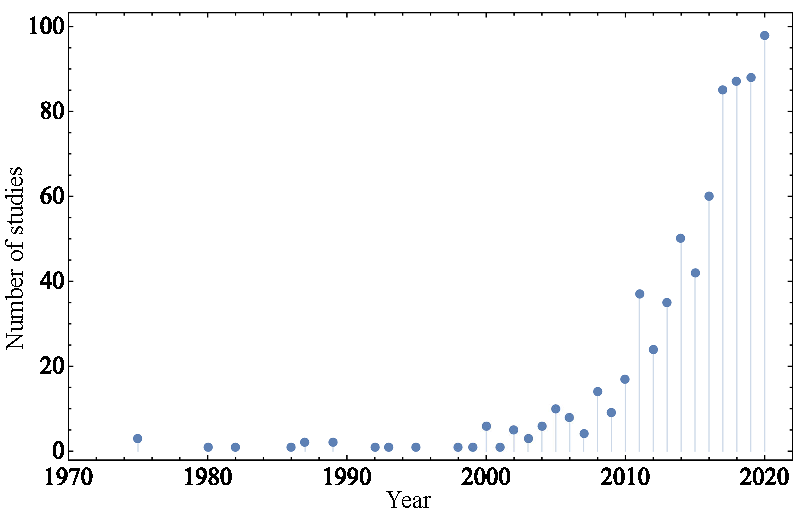
\includegraphics[width=0.9\textwidth]{figs/scopusTrend}
  \caption{Number of publications with keywords ["vortex induced vibration" energy]. Retrieved from SCOPUS.}
  \label{fig:scopusTrend}
\end{figure}

%%Chapter 1-5IE
At the cutting edge of this field of research is a group at The University of Michigan, that has already built prototypes of the energy harvester, named VIVACE (\textbf{v}ortex-\textbf{i}nduced \textbf{v}ibration for \textbf{a}quatic \textbf{c}lean \textbf{e}nergy). They compared the cost of power production in USD/kWh between VIVACE and a wide selection of common (pulverised coal, integrated gasification combined cycle, natural gas combined cycle, etc.) and new power generation technologies (anaerobic digester, landfill gas, solar, etc.). In doing so, they found that VIVACE is on par in terms of power production cost with the other conventional technologies, and published their findings in \citet{Bernitsas2008a}. This result demonstrated VIVACE's economic appeal.
%%Chapter 1-5IE

%%Chapter 1-7IE
The VIV phenomenon utilised by the team at the University of Michigan is of the Karman VIV type (KVIV), capable of producing power in the order of MW when installed as a large-scale energy farm \citep{Raghavan2007a}. Karman VIV - or KVIV for short - is a form of VIV that is induced and sustained by the periodic shedding of Karman vortices from opposite surfaces of a cylinder. The periodic shedding of these vortices creates a pressure fluctuation from the opposing surfaces \citep{Mei2021}. This produces a net fluctuating force acting on the cylinder, which is the lift that drives its vibration. Karman vortices fall into the category of spanwise vortices, and structurally, a single cylinder is all one needs to trigger its formation \citep{Liu2022}.

However, as pointed out by \citet{Koide2013} the reduced velocity ($\ured$) range within which KVIV can be relied upon for power generation is about one order of magnitude smaller than what can be expected from another form of VIV namely the streamwise VIV (SVIV). Reduced velocity $\ured$ is a nondimensional characteristic velocity that allows comparison of results between similar systems vibrating in a flow. Reduced velocity is defined as follows.

\begin{equation}
  \ured = \frac{U_{\infty} \fn}{D},
  \label{eq:reducedVelocity}
\end{equation}

\noindent where $U_{\infty}$, $\fn$ and $D$ refers to the freestream velocity, natural frequency of the system and diameter of the cylinder respectively. Using $\ured$ to express flow velocity allows the reader to gauge how fast the flow is, with respect to the speed of vibration at $\fn$.

%%Chapter 1-9IE<<
Streamwise VIV - or SVIV for short - has its vorticity vector parallel to the direction of the flow. This is different from KVIV whose vorticity vector is perpendicular to the direction of the flow, and is instead parallel to the axis of the cylinder. Structurally, unlike a single cylinder like KVIV, SVIV needs two cylinders in cruciform to trigger its formation. This cruciform is made by placing one cylinder upstream and another downstream. The axes of the two cylinders are at right angles to each other. The midpoint of the cylinders overlap one another, forming a plus sign, i.e. ``$+$''. This type of cruciform, where the two cylinders are at $90 \si{\degree}$ to each other is called the pure cruciform.

Streamwise vortices that drive the vibration of the cylinder appear in pairs, one on the left, and another on the right of the ``$+$''. The streamwise vortex on the left of the ``$+$'' rotates in the opposite direction to the streamwise vortex on the right. This means that the streamwise vortex pair is a counter-rotating pair of vortex. This counter-rotation produces the alternating lift on the upstream cylinder. Since SVIV power generation is possible for a large range of $\ured$, it is better suited for deployment in flows with large velocity changes. to each other is called the pure cruciform.
%%Chapter 1-9IE>>

%%Chapter 1-2EE<<
Unlike KVIV-based energy harvesters, the oscillating upstream cylinder of SVIV-based energy harvesters have both Karman and streamwise vortices shed from it \citep{Koide2017}. This presents a challenge to the measurement of the phase lag between the lift and vibration signals. The closer the phase lag is to $90 \si{\degree}$, the higher the power output \citep{Koide2013,Raghavan2007a}. Hence it is favourable to be able to measure the phase lag as it can help explain an observed improvement or deterioration of the power output. Since both Karman and streamwise vortices are shed from SVIV-based energy harvesters, distinguishing which part of the lift signal is due to either, is difficult. A time-resolved signal processing method is needed and in this study, the Hilbert-Huang Transform (HHT) analysis is employed.

The HHT analysis involves two steps: the first is decomposing a time-series signal into components of decreasing mean frequency, and second, to apply the Hilbert transform on the components to obtain the instantaneous phase \citep{Souza2022}. The application of HHT analysis enables this work to distinguish the dominant components of the lift signal, identify which of these is actually driving the vibration of the cylinder, and compute its phase lag against the vibration signal.
%%Chapter 1-2EE>>

One shortcoming of a SVIV-based harvester is its maximum power output which is demonstrated at the current stage of development to cap at a mW scale for a single-cylinder setup. An isolated cylinder setup for KVIV produces a maximum power in the order of 10 W \citep{Bernitsas2009}. The apparent power $P_a$ (W) for both KVIV and SVIV is shown in Fig. \ref{fig:apparentPowerKoide}. Following this present limitation of the unoptimized SVIV energy harvesters, their application is currently limited to mW electronics e.g., sensors and signal transmitters.

\begin{figure}[!h]
  \centering
  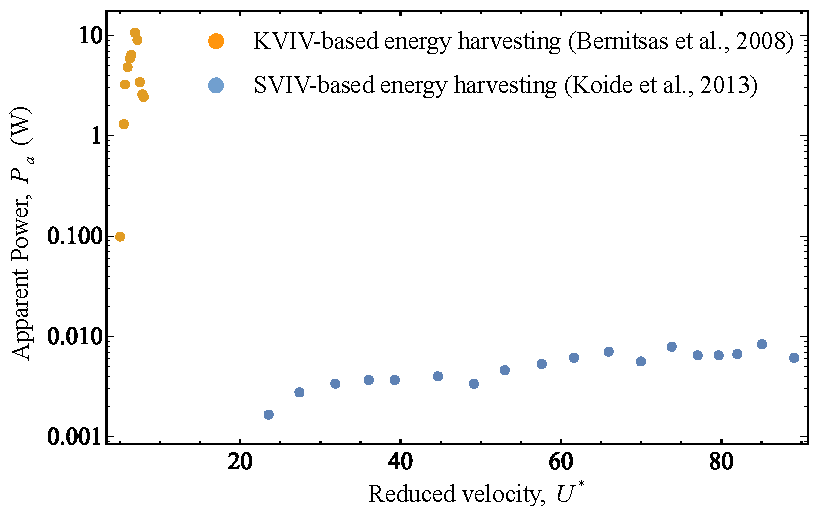
\includegraphics[width=0.9\textwidth]{figs/apparentPowerKoide}
  \caption{Apparent power $P_a $ (W) versus reduced velocity $\ured$ for cases of KVIV and SVIV. Adapted from \citet{Koide2013}.}
  \label{fig:apparentPowerKoide}
\end{figure}

%%Chapter 1-9IE
Nevertheless, these sensors and signal transmitters can make up environment-monitoring sensor networks to monitor the water level in rivers and irrigation canals that benefit flood forecasting efforts. The sensor network can also be used to monitor the level of pollution of the river or canal. This is possible by installing concentration sensors for specific contaminants. Finally, low-power batteries can also benefit from this energy harvesting technology, especially in the context of off-grid charging.
%%Chapter 1-9IE
%%Chapter 1-7IE

%%Chapter 1-3EE<<
 To expand the usability of the cruciform oscillator in energy harvesting, efforts should be made to improve its power output. Hence, this thesis seeks to identify the cause that limits the power output to its current value. This includes the identification of vortical structures in the flow, their location, and strength. The thesis also looks into the modulation of the lift signal by the shedding of vortical structures. Then, this thesis seeks to explore a new parameter in the study of the cruciform oscillator, which is the cruciform angle. This study documents the effects of the various cruciform angles on the vortical structures present in the flow in terms of their location and strength. In addition, this work also studies their effects on the lift and vibration signal, and ultimately, estimated power output and efficiency.
 %% Chapter 1-3EE>>

% One of the most immediate uses of such sensors in Malaysia is part of a flood early warning system. Flood forecasting is possible without much difficulty using conventional methods if there is a sufficient number of hydrological observatories along the body of water \citep{DIDMalaysia2010}. For this to take place, electricity must be available to run the observatories, in addition to favourable terrain near the body of water to house the equipment.

% In urban areas, even though sourcing electricity may not be a hurdle, placement of the observatory itself can be, due to land ownership issues. Nevertheless, these issues do not in any way lessen the need to have an adequate number of observatories in urban areas. After all, urban areas are known to bear a greater risk of flash floods compared to rural areas owing to disrupted natural systems of runoff production as a result of poorly planned development \citep{Abdullah2004,Takaijudin2010,Abdullah2011}. Therefore, the prospect of devising a simple river monitoring system that consists of only a few sensors and electronics totalling to a maximum combined number of three (3), powered by a TVIV energy harvester hence becomes worthy of further inquiry.

\section{Problem Statement} \label{sec:probState}

The preceding section has established the viability of harnessing energy from a flow by exploiting the VIV phenomenon. Multiple modes of VIV have been observed, and SVIV stands out as better oriented for deployment in fluid flows that vary greatly in terms of free-stream velocity. Even with very rudimentary optimisations, SVIV from a cruciform harvester has the ability to generate power in the order of mW consistently over a large range of free-stream velocities \citep{Koide2013}.

% This can be harnessed to develop a self-contained river monitoring device that deploys with ease, especially in urban neighbourhoods to facilitate early warning of floods.

To achieve this, the problems outlined below must be addressed to close relevant gaps in the current body of knowledge.

\begin{enumerate}
  \item A lack of understanding on the transition mechanism from Karman to streamwise vortex-induced vibration.
  \item A paucity in the knowledge on what contributes to the magnitude of the alternating lift force acting on the cylinder, and its vibrational frequency components.
  \item A deficiency of new methods to control the flow perturbation which gives rise to a strong, stable and periodic forcing of the cylinder vibration, sustainable over the desired operating range of $\ured$.
\end{enumerate}

%%Chapter 1-5EE<<
Problem statement one stems from the realisation that although past studies have shown that SVIV in a cruciform harvester begins around $\ured = 18$ \citep{Koide2013}, none has ever looked into how the transition actually occurs from KVIV. This is especially the case in terms of the distribution of vortical structures around the cruciform, the lift signal: its frequency, amplitude and phase lag relative to the cylinder vibration signal. Removing this lack of understanding can help to trigger the desired mode of vibration at a lower $\ured$.

Problem statement two stems from the observation by \citet{Zhao2018a} on sectional lift, which drew attention to the effect a vortical structure has on the lift acting on the cylinder. Particularly in the case where several types of vortices are being shed simultaneously - like the cruciform harvester - the paucity in the knowledge on how the different vortical structures affect the lift signal is a hindrance to improving the maximum lift that can be possible obtained from the cruciform harvester.

Finally, problem statement three comes from the realisation that recent studies in the field of cruciform energy harvester seems to be hard-pressed in finding new parameters to explore, focusing time and again on the gap between the cylinder and the downstream plate, the plate width and other dimensions of the system \citep{Sakamoto2021}.

To date, the upstream and downstream cylinder (or plate) in cruciform harvesters have always been assumed to be at $90 \si{\degree}$ to each other. It is possible that keeping the cruciform at a right angle prevents the discovery of other configurations that are capable of outputting higher power at better efficiencies. With enough cruciforms studied between angles $0 \si{\degree}$ and $90 \si{\degree}$, one can synthesise a map of power and efficiency of cruciform harvesters at various cruciform angles $\alpha \; (\si{\degree})$ that can advise on the selection of the cruciform harvester for a given design constraint.
%%Chapter 1-5EE>>

\section{Research Questions} \label{sec:resQue}
The answer to several questions is sought in this proposed study. These questions are meant to drive the study towards its objectives.
\begin{enumerate}
  \item How does the lift signal evolve as the flow transitions from being driven primarily by Karman vortex to streamwise vortex?
  \item How does the ratio of energy transferred from the flow to the lift components evolve with respect to $\ured$?
%%Chapter 1-9IE<<
  \item Compared to a pure cruciform, what are the differences the Karman or streamwise vortical structures experience under the condition of a modified cruciform? \label{enum:deviation}
  \item How do the differences mentioned in \ref{enum:deviation} affect the lift magnitude, and by extension the frequency-amplitude response?
%%Chapter 1-9IE>>
  \item Where in the power envelope can maximum (minimum) power be obtained with the largest (narrowest) operability range, and how does this translate into a new mode of flow control to suit the operating conditions of the cruciform energy harvester?
\end{enumerate}

\section{Thesis Objectives} \label{sec:thesisObj}
Following the problems outlined in the previous section, the objectives that define the scope of work in this proposal are listed below.

%%Chapter 1-10IE<<
\begin{enumerate}
  \item To identify the causes of the difference in amplitude and frequency response of the lift and vibration signals when the dominant vortical structure changes from Karman to streamwise vortex, in a pure cruciform. \label{enum:whatHappens}

  \item To distinguish the dominant components of the lift signal and how the components interact to modify the amplitude and frequency response of cylinder vibration, in a pure cruciform. \label{enum:characteriseLift}

  \item To synthesise a map for each of the amplitude, power, and efficiency, summarised in the cruciform angle $\alpha \; (\si{\degree})$ - reduced velocity $\ured$ parameter space. \label{enum:passiveControl}
\end{enumerate}
%%Chapter 1-10IE>>

%%Chapter 1-6EE<<
As mentioned previously in Section \ref{sec:probState}, there is a lack of understanding on how the transition from KVIV to SVIV takes place in a cruciform energy harvester, which is the first problem statement. The first objective is thus to establish the relationship between the amplitude and frequency response of the lift and vibration signals and the vortical structures that are present at that time. The amplitude response is computed by taking the root-mean-square of the signals, both lift and vibration, and plotting them against $\ured$. The frequency response is computed by finding the dominant frequency in the FFT spectrum of the signals, both lift and vibration. Vortical structures are identified by computing the vorticity field.

Then, the second objective of distinguishing the dominant components of the lift signal is to answer problem statement two. As the reason behind the modulation of the lift signal remains unknown, this objective seeks to analyse the lift signal. The method of analysis to be employed here is HHT, through which the signal can be decomposed and the dominant components identified. Once the components of lift have been identified, the study can explain how they interact to produce the amplitude and frequency response of the cylinder vibration being observed.

Lastly, the third objective of synthesising a map of the vibration amplitude, power and efficiency in the $\alpha \; (\si{\degree})$ - reduced velocity $\ured$ parameter space is stated to answer problem statement three. As mentioned in problem statement three, the fact that studies have always assumed the cruciform oscillator to have a cruciform angle of $90 \si{\degree}$ has prevented the investigation of a generalised cruciform oscillator. By computing the amplitude response, power and efficiency of a few cruciforms between $0 \leq \alpha \; (\si{\degree}) < 90$, this study will be able evaluate the feasibility of varying the angle of the cruciform as a method to control flow perturbations due to the arrangement of vortical structures around the cruciform. This also provides a guideline for the optimal cruciform angle for a given design constraint such as vibration clearance, structural integrity and operating range of $\ured$, in addition to power output and efficiency.
%%Chapter 1-6EE>>

\section{Scope of Works} \label{sec:scopeWork}
%%Chapter 1-12IE<<
This work is a mainly a computational fluid dynamics (CFD) study of a particular version of VIV-based energy harvester that comprise of an elastically supported, horizontally constrained smooth circular cylinder of diameter 1 cm and a passive flow control mechanism that is a strip of rectangular plate at a right angle downstream the cylinder, forming a cruciform. The range of Reynolds number investigated in this thesis is between $1.1 \times 10^{3} \leq \text{Re} \leq 14.6 \times 10^{3}$ and the mass-damping parameter, expressed by the nondimensional Scruton number Sc, is 9.94. This work limits itself to examining a cruciform where the width of the strip plate is equal to the diameter of the cylinder $D$, and the primary data collected from the simulation runs are the time evolution of the cylinder displacement and the corresponding lift coefficient Cl.

The baseline numerical results, i.e. results from a pure cruciform (a cruciform where the cylinder and strip plate are \SI{90}{\degree} to each other) are validated against experimental results of a similar system in a custom-made recirculating open flow channel. This experiment to validate the baseline numerical results also used a 1 cm diameter circular cylinder. A strip plate of width 1 cm was placed downstream the circular cylinder at a $90 \si{\degree}$ angle. Data collected from the experiment is limited to the vibration signal (i.e., cylinder displacement) only, and only between $1.1 \times 10^{3} \leq \text{Re} \leq 11.2 \times 10^{3}$. The vibration signal is then post-processed into their respective amplitude and frequency responses.

The simulation in this study collects data on the three-dimensional pressure and velocity fields, and also cylinder displacement data. The pressure field is then post-processed to obtain lift signal acting on the cylinder, while the velocity field is post-processed to obtain the vorticity field. This is in relation to objective one that seeks to establish the amplitude and frequency responses of the lift and cylinder vibration signals. This is different from the parameters studied in \citet{Koide2017}, as in their experiment, they only seeked to visualise the different vortical structures that appear between $1.2 \times 10^{3} \leq \text{Re} \leq 5.7 \times 10^{3}$ for cruciforms with different cross-sectional shapes.

On the other hand, the study by \citet{Zhao2018a} only looked into the visualisation of the vortical structures around the cruciform and the distribution of lift along the vibrating cylinder. The range of Reynolds number they studied was between $1 \times 10^{2} \leq \text{Re} \leq 5 \times 10^{2}$. This distribution of lift along the length of the vibrating cylinder reveals the location of dominant vortical structures and helps to visualise their strength with respect to time. Instead, this thesis used the FFT of the transverse (direction parallel to the vibration of the cylinder) velocity component downstream the cylinder to visualise dominant vortical structures and their strength.

This thesis looks to discover the relationship between the vortical structures present in the flow and how they modulate the resulting lift acting on the vibrating cylinder of the pure cruciform. Special focus is given to the high flow velocity region where SVIV takes place. This is done by conducting a time-series analysis of both cylinder displacement and lift coefficient signals using the Hilbert-Huang transform (HHT). The motivation behind this is to understand why the amplitude of cylinder displacement is limited to the order of magnitude observed not only by the author, but also in numerous studies within the last ten years. This part of the study concludes with the discovery of a particular route through which a significant amount of energy from the freestream is lost during the energy harvesting process, and the amount by which the power output can be improved if this loss is eliminated. This scope is related to objective two.

The second part of this thesis is the author's attempt to eliminate the loss mentioned previously. This is done by generalising the cruciform system, through the variation of the relative angle between the cylinder and the strip plate. The study then proceeds to investigate the generalised cruciform system by examining the vortical structures present in the flow, how they affect the resulting lift acting on the cylinder, the amplitude of cylinder displacement itself, and ultimately the power output. The dynamics between the lift and cylinder displacement are explained through the computation of instantaneous phase lag between the two, which in turn is made possible by HHT.

The thesis concludes with the unveiling of a mechanical power and efficiency map, within a parameter space consisting of the cruciform angle and $\ured$. Useful recommendations can be deduced from the map, which highlights regions of high and low power output, and also regions of high and low efficiency, in order to obtain the desired power output and efficiency for any given power consumption requirement. This scope is related to objective three.
%%Chapter 1-12IE>>

\section{Significance of Study} \label{sec:signStudy}
%%Chapter 1-11IE<<
The aim of objective \ref{enum:whatHappens} is to get a better understanding on SVIV in a pure cruciform. A better understanding of SVIV in a pure cruciform in important because this is the baseline case, to which the performance of other cruciforms at different cruciform angles will be compared. Achieving this objective can demonstrate how the inception of streamwise vortical structures perturb the amplitude and frequency of lift, which directly modifies the amplitude and frequency of the cylinder vibration.

Next, achieving objective \ref{enum:characteriseLift} is desirable because it allows the establishment of a direct link between the different branches of KVIV or SVIV and how the vortices modulate the lift signal of a pure cruciform. Apart from that, distinguishing the dominant components of lift allows us to quantify how much energy from the flow is consumed by each of the Karman or streamwise vortices, and in return, how much do they contribute towards driving the vibration of the cylinder. Investigating this for the pure cruciform lay the grounds to understand how power generation is affected by the configuration of vortices in the flow for more complex situations, i.e., when the cruciform angle is no longer $90 \si{\degree}$.

Finally, objective \ref{enum:passiveControl} is significant because in achieving it, one is able to evaluate and recommend the optimal cruciform angle for the designated specifications for vibration clearance, power output and efficiency. This holds the key as to how the cruciform angle should be varied to cater to a particular flow environment and structural integrity - much like the performance curves associated with engines and pumps.
%%Chapter 1-11IE>>

% As a whole, Malaysia receives an average rainfall of about 2990 mm annually (Harris et al., 2014). East Malaysia registers an approximate 3250 mm - nearly 1000 mm in excess of the average rainfall figures for west Malaysia which is about 2500 mm \citep{DIDMalaysia}. Contribution to these values is greater during the monsoon seasons which occur during the months of November to March (north-west monsoon) (Kuala Lumpur Monsoon Activity Centre, 2015) and May to September (south-west monsoon) \citep{Billa2004}. The increased rainfall during the monsoon season inevitably saturates catchments, producing several times the usual amount of runoff that rivers can drain to the sea within sufficient time \citep{Chia2004}. Consequently, water lever rises past the river banks and progresses into the surrounding terrain. This is how floods commonly come into being during the monsoon season.

% Outside the monsoon season, the inception of floods is due to convective rainfall. The flood frequency and extent due to convective rain are worse in an urban setting compared to rural areas. The underlying cause of this is none other than the major disruption of pre-urbanization mechanisms that govern the original rainfall-runoff processes of an area. Thus, crippling floods can manifest within a matter of hours from the start of rainfall, i.e. flash floods.

% Off-grid charging of electronics is also another area to which the results of this study is able to improve. Both civilian and military activities in remote areas can benefit from the power generated to charge essential electronic devices necessary for a successful operation in said area. Improvement in terms of power output means that usage of more complex and resource intensive electronic equipments will gradually be possible in off-grid locations. This gives the deployed personnel an added advantage over their peers in performing his or her civilian or military duties in such locations.

% The most significant contribution is however, to facilitate the widespread adoption of independent, wireless sensor networks. Sensor networks have wide-ranging applications in the field of monitoring; from wildlife \citep{Gazis2020,Pathak2020} to forests \citep{Kadir2019,Zellweger2019} to civil structures \citep{Ni2020,SadeghiEshkevari2020,Mao2020}, these networks are low-power by design and is expected to operate around the clock. To increase the coverage and resolution of the monitoring task, the obvious solution is to increase the overall quantity and concentration of sensors in a particular area of interest. Nevertheless, the impracticality of connecting such a network to the national grid thrusts them in a unique position to benefit from VIV-based energy harvesters that this study seeks to improve upon.
\section{Thesis Organisation} \label{sec:thesisOrg}
%%Chapter 1-13IE<<
This thesis is organised into eight chapters. The author introduces the study and gives a general overview of the research in Chapter 1. In Chapter 1, gaps in the research are identified and thesis objectives are formulated based on those gaps. Chapter 1 also outlines the questions the author seeks to address, details the scope of this study and provide concrete examples as to the significance and merit of this work. Chapter 2 reviews relevant literature that gives an overview of the progress made up to the present day, on the subject of VIV energy harvesting, by exploiting an isolated circular cylinder as the oscillator. The chapter then introduces the cruciform oscillator and the studies on the vibration characteristics of a number of variations of the cruciform oscillator.

Chapter 3 discusses the methodology taken by the author to attain the objectives listed in Chapter 1. In Chapter 3, the author details the numerical model implemented in the CFD undertaking and this includes the domain size, critical dimensions of the cruciform, boundary conditions and solution method to the unsteady, three-dimensional (3D) Reynolds-averaged Navier-Stokes equation governing the flow. Apart from that, the author also discusses the turbulence modelling adhered to in the numerical studies. The author also introduces the Hilbert-Huang transform (HHT) and explains the ensemble empirical mode decomposition (EEMD) algorithm that drives the decomposition of a time series signal into a finite number of orthogonal components. Finally, the author explains the Hilbert transform and how the transform is able to compute instantaneous phase or frequencies of a decomposed component of the signal.

Chapter 4 first takes into account the validation of the numerical setup in two ways: by way of a grid independency study, and by way of experimental comparison. The grid independency study utilises the Richardson extrapolation and grid convergence index (GCI) as the primary tool to ensure spatial convergence of the numerical results. In the experimental validation, this work showcases a simple contactless method of measuring the cylinder displacement using a camera and an open-source image tracking software. After the processing of the experimental data to compute the uncertainty and present them as error bars, the author concluded that the numerical results of the pure cruciform (\SI{90}{\degree} cruciform) is in fair agreement with the experimentally obtained values, providing an added layer of confidence in the numerical results.

This is then followed by the vibration characteristics of a pure cruciform. In this section, the author studies in detail the lift-displacement dynamics that results from the kind of vortical structures that appear in this setup. This section concludes with the discovery of a path to energy loss that has never been considered before in the literature and estimated the amount of improvement possible for the power output if said loss is eliminated.

Then, the chapter continues to discuss the vortical structures and lift-displacement dynamics of a steep-angled cruciform ($45 \le \alpha (\si{\degree}) \le 67.5$), followed by the vortical structures and lift-displacement dynamics of a shallow-angled cruciform ($0 \le \alpha (\si{\degree}) \le 22.5$). Here, the study found out that for shallow-angled cruciforms, the onset of meaningful power generation is brought down significantly to from $\ured = \urei$ in the pure cruciform, to $\ured = \urfo$ when the cruciform angle is $\angon$. At $\alpha = \angon$, the maximum power also improves by approximately a power of two.

Finally, the author computes the mechanical power and efficiency of each of the cruciform variants for all flow velocities studied. From it, this work is able to produce a mechanical power and efficiency map, in essentially a cruciform angle-flow velocity parameter space.

Chapter 5 details the conclusions that follow the discussions made in Chapter 4. Here, the four main findings of this work are summarised and the chapter ends with some remarks on potential future works for this study.
%%Chapter 1-13IE>>

\chapter{Literature Review} \label{chap:literatureReview}
The alternate shedding of vortices from opposing sides of a cylinder introduces an alternating lift and drag which, unless constrained, will induce the vibration of the cylinder. This vibration energy can be converted into electrical power via the piezoelectric effect or electromagnetic induction. This is the basis of vortex-induced vibration (VIV) energy harvesting, and in this chapter, the author goes through the body of work done on the subject of vortex shedding, vortex-induced vibration and finally energy harvesting from the many variants of cylindrical oscillators, to determine the limits of the current knowledge and pinpoint where this work resides within the web of research done by the community.

\section{Vortex Shedding from a Cylinder}
% In this work, a cylinder is defined as an elongated three-dimensional (3D) object with a well-defined axis, and whose cross-sectional shapes are the same at any arbitrary location along the axis. Flow around a cylinder is one of the phenomenon that, although abundantly occurring in nature and in man-made settings, remains impervious to rigorous and analytical description of the phenomenon. Key to this elusiveness is the fact that for a flow pattern to manifest itself in the physical world, the solution to the governing equations of fluid mechanics must not only exist, but must also be stable to ambient random excitations for it to be sustainable. Thus far, the Navier-Stokes equation remains unsolved on the list of Millennium Problems by the Clay Mathematics Institute, prompting researchers to rely heavily on experimental and numerical techniques in the push for breakthroughs in this field of study. Vortex shedding from a cylinder is one such interest in this field - and as the reader will see in the following subsections - whose advances are greatly driven by experimental and numerical research.

%%Chapter 2-1IE<<
Numerous occurrences of VIV are readily observable in the field of engineering. In the ocean, marine currents give rise to the vibration of risers and offshore drilling platforms. For example, the marine risers reviewed by \citet{Liu2020} in their review paper on recent progress in the research on vibration control of marine risers. Marine risers are also the subject of the study by \citet{Zhang2020}, where they investigated the feasibility of applying tension to the top of the riser as a method to control its vibration. Another example of marine risers in the study of VIV can be found in \citet{Meng2020}, where they looked into the modes of VIV that manifest themselves in flexible risers.

% Up in the sky, aeroplane wings vibrate, and high-rise buildings experience sway as strong gusts blow around the mighty structures \citep{Arul2020,Hao2020,Gao2020}. Closer to the ground, power transmission lines vibrate as the result of wind blowing over them \citep{Wang2019,Gomez-Ortega2019a}.

On dry land, VIV is observed to produce vibration of power transmission lines. This can be found in the study by \citet{Gomez-Ortega2019a}, where they studied the vibration of transmission lines experimentally, that is caused by VIV. Power transmission line vibration also appeared in the analytical work by \citet{Gomez-Ortega2019b}, where they proposed a mathematical model that describes the vibration of the transmission line. These studies demonstrate the usual motivation that drives the study of VIV. As exemplified by these studies, VIV phenomenon is so common in the engineering field that a huge amount of effort goes into suppressing it. This availability of VIV that is so common in engineering initiated the movement to instead maximise it, and use it for energy harvesting \citep{Barati2022}.

As the name suggests, VIV is the result of the periodic shedding of vortices. This chapter will thus begin with a review of the most common form of vortex shedding: Karman vortex shedding.
%%Chapter 2-1IE>>

\subsection{Karman Vortex Shedding} \label{ssec:kvShedding}
The formation of Karman vortex is the direct result of flow separation over a body submerged in a fluid flow. At low Reynolds numbers, the streamline is still able to follow the contour of the submerged body due to viscosity.  Here, the Reynolds number Re of the flow is defined as

\begin{equation}
  \text{Re} = \frac{UD}{\nu},
  \label{eq:reyNum}
\end{equation}

\noindent where $U$, $D$, and $\nu$ are the characteristic velocity, characteristic length, and the kinematic viscosity of the fluid, respectively. For the case of the flow around a circular cylinder, $U$ denotes the flow velocity and $D$ the diameter of the circular cylinder.

As the Reynolds number increases, the higher inertial forces in the flow overpower the viscous forces that kept the streamline along the surface of the body, causing it to separate. This separation creates a bubble downstream the body. With further increase in Reynolds number, the bubble destabilises, leading to the formation of vortices that are shed alternately from the top and bottom surfaces of the body. This evolution of vortex shedding behaviour with respect to Re is summarised in Fig. \ref{fig:karmanVortexEvolution}. For creeping flows with $\re < 5$, the flow streamline follows the curvature of the circular cylinder submerged in the flow. Then, between $5 \leq \re < 40$, a small recirculation bubble forms at the downstream side of the circular cylinder. Further increasing the value of $\re$ destabilises the bubble, leading to the the shedding of Karman vortices. Karman vortex shedding becomes turbulent between $150 \leq \re < 30 \times 10^{5}$.

%%Chapter 2-7IE<<
\begin{figure}[!h]
  % \centering
  \hspace{1.3cm}
  \begin{subfigure}[h]{0.25\textwidth}
    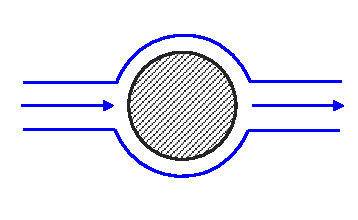
\includegraphics[width=\textwidth]{figs/karmanVortex0-5}
    \caption{$\re < 5$}
    \label{fig:kv05}
  \end{subfigure}
  \hspace{4cm}
  \begin{subfigure}[h]{0.25\textwidth}
    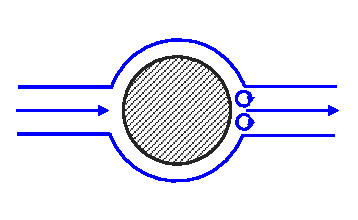
\includegraphics[width=\textwidth]{figs/karmanVortex5-40}
    \caption{$5 \leq \re < 40$}
    \label{fig:kv540}
  \end{subfigure}

  \begin{subfigure}[h]{0.45\textwidth}
    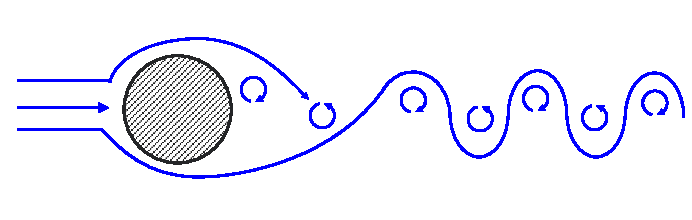
\includegraphics[width=\textwidth]{figs/karmanVortex40-150}
    \caption{$40 \leq \re < 150$}
    \label{fig:kv40150}
  \end{subfigure}
  \hspace{1cm}
  \begin{subfigure}[h]{0.45\textwidth}
    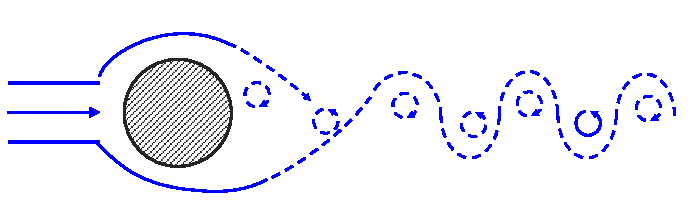
\includegraphics[width=\textwidth]{figs/karmanVortex150-30k}
    \caption{$150 \leq \re < 30 \times 10^{5}$}
    \label{fig:kv15030k}
  \end{subfigure}
  \caption{Evolution of Karman vortex shedding from a two-dimensional circular cylinder at increasing Reynolds number.} \label{fig:karmanVortexEvolution}
\end{figure}
%%Chapter 2-7IE>>

In the study of Karman vortex shedding, seldom is the case where one does not find reference being made to a chart on lift and drag coefficients for a stationary circular cylinder between $10^{0} < \text{Re} < 10^{8}$ in \citet{Zdravkovich1997}. The lift coefficient $\cl$ acting on the body is defined as

\begin{equation}
  \cl = \frac{\fl}{\frac{1}{2}\rho U^{2} A},
  \label{eq:clDef}
\end{equation}

\noindent where $\fl$, $\rho$, $A$, and $U$ are total lift force acting on the body, density of fluid in which the body is submerged, area of the surface of the body, and characteristic velocity, respectively. Similarly, its drag coefficient is defined as

\begin{equation}
  \cd = \frac{\fd}{\frac{1}{2}\rho U^{2} A},
  \label{eq:cdDef}
\end{equation}

\noindent where $\fd$ is the total drag force acting on the body instead. By convention, the direction of the lift and drag are defined relative to the mean direction of the flow, i.e., the freestream. The lift force is normal to the freestream, while the drag force, parallel to the freestream.

The observation by \citet{Zdravkovich1997} that both lift and drag coefficients ($\cl$ and $\cd$) have their high and low regions within $10^{0} < \text{Re} < 10^{8}$ is of extreme utility to engineers. From the preservation of risers to the improvement of power output for VIV-based energy harvesters, the chart in \citet{Zdravkovich1997} gives a rough outline to the range of Reynolds number suitable for a particular engineering operation. This chart is presented in Fig. \ref{fig:zdravkovichMap}, with the highlighted region showing the Re range studied in this thesis. That being said, the chart remains silent on why $\cl$ and $\cd$ evolve the way they do with respect to Re, leaving the gap to be filled by later researchers.

\begin{figure}[!h]
  \centering
  \hspace{1cm} 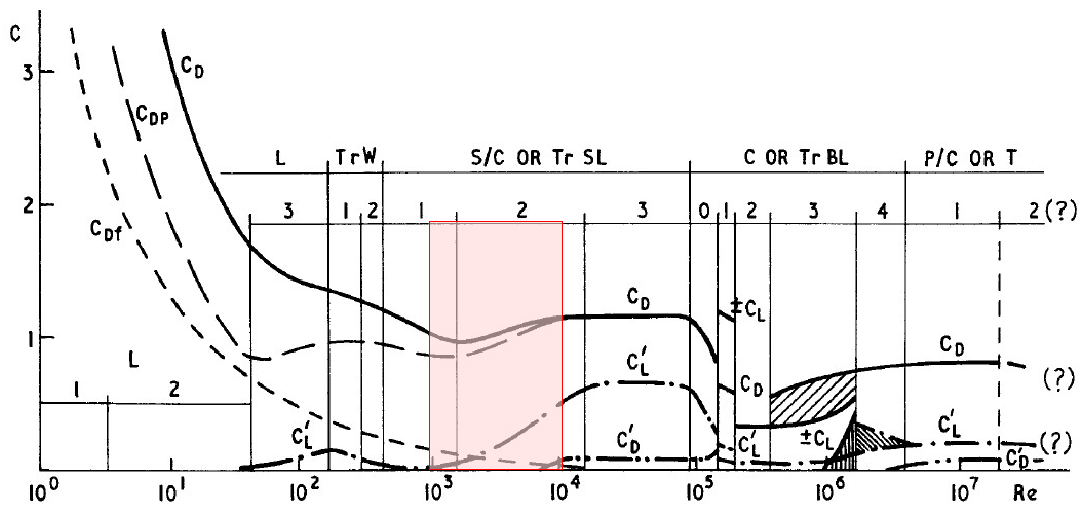
\includegraphics[width=0.9\textwidth]{figs/zdravkovichMap}
  \caption{Force coefficients versus Re summarised by \citet{Zdravkovich1997}.}
  \label{fig:zdravkovichMap}
\end{figure}

For example, \citet{Desai2020} tackled the question why is there a reduction in $\cl$ and $\cd$ as the cylinder goes through the upper boundary of subcritical flow ($1.49 \times 10^{5} < \text{Re} < 3.55 \times 10^{5}$). Their study is experimental, using tools such as particle image velocimetry (PIV) for a quantitative visualisation of the two-dimensional (2D) flow field, and proper orthogonal decomposition (POD) for identification of dominant flow structures. In doing so, they have identified two modes of shedding - the antisymmetric and symmetric modes - which takes place one after another, albeit in no well-defined cycle. The antisymmetric mode corresponds to the ``normal'' shedding of Karman vortices while the symmetric mode a weaker form of shedding with a higher energy level in its low-frequency components. The symmetric mode gains strength with increasing Re, which entails a weaker form of shedding taking over the flow. This ultimately reduces the magnitude of $\cl$ and $\cd$ of the cylinder. Depending on which side of the divide one is, an engineer may opt to amplify the symmetric mode to protect the integrity of a structure, or augment the antisymmetric mode to improve the conversion efficiency of energy from the freestream into cylinder vibration. In other words, a deeper understanding into the mechanics of Karman vortex shedding invariably leads to better strategies in cylinder motion control.

Expanding on the topic of flow control, \citet{Durhasan2019} conducted an experimental study of the shedding process under the following setup: the circular cylinder is placed in a larger hollow cylinder with varying pore spacing - quantified by their porosity - $\beta$ - and submerged in a water flow at Reynolds number $\text{Re} = 5000$. What they found out is the stunting of the wake from the inner cylinder when $\beta \leq 0.5$, while for porosities $\beta \geq 0.6$, a reduction of 21\% to 87\% in drag is observed. It is worth noting that both lift and drag forces are equally able to initiate the vibration of the cylinder.

Another exploitation of porous material in the control of Karman vortex shedding is in the work of \citet{Geyer2020}. In \citet{Geyer2020}, they work to test a method of noise reduction by wrapping certain parts of the cylinder surface with a porous material. This is because, at velocities in the order of $O(10^{1})$ m/s, Karman vortex shedding also exacerbates the level of noise generated by the cyinder. They discovered that the higher the air resistance of the material, and the higher the porosity, the bigger the improvement will be in terms of noise reduction. In addition, the porous wrapping reduces turbulence intensity in the wake near-field, hence making it more uniform.
%%Chapter 2-4IE<<
This goes to show that the vibration that results from Karman vortex shedding can manifest itself at different scales. First, on the high-amplitude, low-frequency scale, where it is observed as the motion of the cylinder. The second in on the low-amplitude, high-frequency scale, where it is observed as noise generation. It should be stressed, however, that both are simply the different scales of vibration that results from the shedding of Karman vortex.
%%Chapter 2-4IE>>

In studying a flow around a solid object, one quickly finds that experimental methods employed in the investigation is never absolutely independent of the phenomenon being studied. The use of probes, for example, means that the researcher is introducing additional elements into the flow that cannot be fully isolated from affecting the flow, however careful the design of the experiments are. To compensate this shortcoming, studies have employed numerical methods to model the flow under consideration, and track the evolution of quantities of interest in the flow to a degree of resolution limited only by the computational power available. Taking note of the expediency of porous media buffering the cylinder to temper flow behaviour, \citet{Ledda2018} made use of numerical methods to simulate Karman vortex shedding from a square cylinder to gain a deeper insight on how the flow interacts with the porous media to produce the flow responses discussed previously. In this study, the authors observed the efficacy of a porous cylinder surface in not only detaching the recirculation region in the near-wake, but in purging it altogether, at higher porosity values. If a technique can be found to vary the the porosity of the surface, perhaps through the use of smart materials \citep{Arsh2020}, an engineer can basically switch Karman vortex shedding on and off at will.

%%Chapter 2-5IE<<
Other than the usual methods of numerical investigation that work to solve the continuity and Navier-Stokes equations directly (DNS) \citep{AlvesPortela2020}, or those that employ some form of simplification \citep{Shao2016}, methods that model molecular dynamics (MD) have also found their way in the arsenal of tools available to researchers in the field of fluid-structure interaction. One such example is the study by \citet{Asano2020}. In it, the authors employed the Lennard-Jones potential to model represent the molecular dynamics of a flow around one or two circular cylinders. The Lennard-Jones potential models the fluid particle distribution, and all physical quantities are then expressed in terms of energy, length and time. What they discovered was, cavitation, although undesirable in normal operation of turbomachineries, can be a determining factor in the onset of Karman vortex shedding. As they decreased the fluid temperature, the cavitation bubbles interact with the shear layer of the cylinder in a manner that pushes the wake further downstream than usual. Eventually, wake where the vortex shedding resides is pushed far enough downstream that the alternating lift that normally acts on a cylinder during Karman vortex shedding vanishes.
%%Chapter 2-5IE>>

Another method for Karman vortex shedding control that imposes some form of modification to the shear layer of the cylinder is through the affixing of fairings on the surface of the cylinder. A recent example of this can be found in the work of \citet{Kang2020}. In \citet{Kang2020}, the fairings affixed to the cylinder surface caused a reduction in both lift and drag acting on the cylinder, although the strength of this effect varies with respect to the actual flow velocity being imposed on the cylinder.

Apart from tempering the shear layer of the cylinder, one can also - similar to \citet{Yokoi2016} - alter the downstream region of the cylinder to achieve a desired response. In their study, \citet{Yokoi2016} introduced a splitter plate on the trailing edge of a circular cylinder and discovered a rich collection of flow patterns that one can achieve simply by varying the following variables: splitter plate length, cylinder forcing amplitude and cylinder forcing frequency. By doing this, one can even achieve a symmetric shedding of Karman vortices from the top and bottom surfaces of the cylinder. To appreciate the significance of this result, one simply needs to recall that alternating $\cl$ and $\cd$ acting on the cylinder is the consequence of Karman vortices shedding alternately from the top and bottom of the cylinder. The fact that one can force the shedding to take place simultaneously from the top and bottom of the cylinder means that the amplitude of both $\cl$ and $\cd$ can be significantly diminish, if not altogether.

To be clear, the splitter plate method is not particularly new in near-wake control; splitter plates have been studied in the past under a similar setup \citep{MatAli2012}, although under completely different flow conditions and cylinder geometry. However, one may find it difficult not to rely to some extent on the studies by \citet{MatAli2012}, since unlike \citet{Yokoi2016}, they study flow patterns that are self-induced and does not rely on external forcing. This is particularly pertinent as in nature and man-made settings, self-induced vibrations is the norm rather than the exception.

\subsection{Streamwise Vortex Shedding} \label{ssec:svShedding}

%%Chapter 2-8IE<<
In the real world, Karman vortex shedding is almost never a two-dimensional phenomenon. Once Re exceeds 150, Karman vortices can no longer be considered a purely two-dimensional vortical structure, with its vortex line parallel to the axis of the cylinder from which it is shed. The stretching of Karman vortex lines in the direction of flow breaks the two-dimensionality as there are now sections of the vortex line that points in the direction of the flow. The sections of the vortex line that now points in the direction of the flow - or stream - create structures that are called streamwise vortices. A schematic of this vortex line stretching is presented in Fig. \ref{fig:modeAStretching}.

\begin{figure}[!h]
  \centering
  \hspace{1cm} 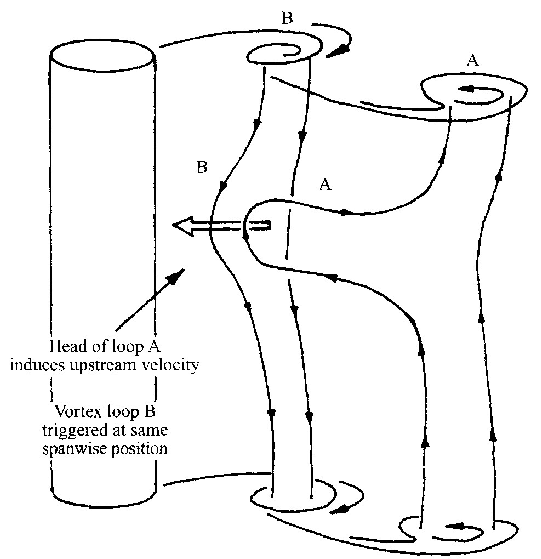
\includegraphics[width=0.5\textwidth]{figs/modeA}
    \caption{Stretching of the vortex line on a Karman vortex creates streamwise vorticity. Adapted from \citet{Williamson1996a}.}
    \label{fig:modeAStretching}
  \end{figure}

Among the studies on Karman vortex three-dimensionality are the works of \citet{Williamson1996a} and  \citet{Williamson1996b}. The author discusses two main modes of three-dimensionality: modes A and B. Mode A has a spanwise wavelength of three to four diameters and appears at $\re = 200$. Mode A of Karman vortex shedding is visualised in Fig. \ref{fig:modeA3D}. The streamwise vortices are the vortical structures whose axis is parallel to the freestream.

\begin{figure}[!h]
  \centering
  \hspace{1cm} 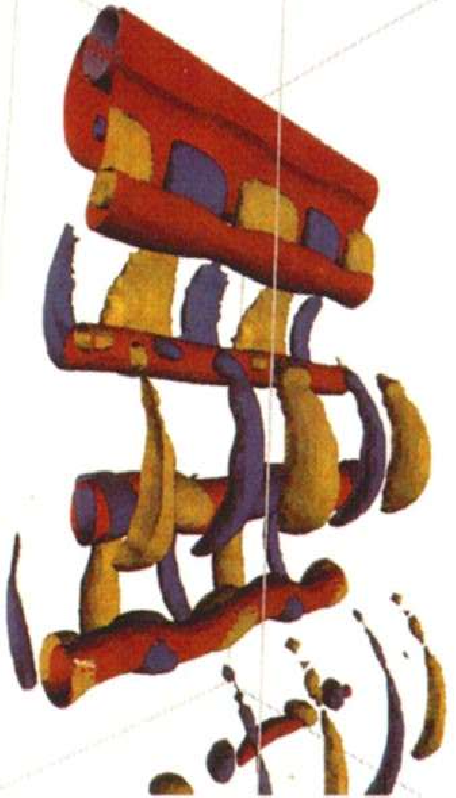
\includegraphics[angle=90,width=0.7\textwidth]{figs/modeA3D}
    \caption{Three-dimensional visualisation of mode A of Karman vortex shedding. Adapted from \citet{Thompson1994}.}
    \label{fig:modeA3D}
  \end{figure}

However, as Re is increased, another mode with a smaller wavelength appears, designated as mode B. The modes consist of vorticities that point in the streamwise direction. The shedding of these modes are therefore a simple representative case of streamwise vortex shedding. On the other hand, mode B Karman vortex shedding is shown is Fig. \ref{fig:modeB3D}.

\begin{figure}[!h]
  \centering
  \hspace{1cm} 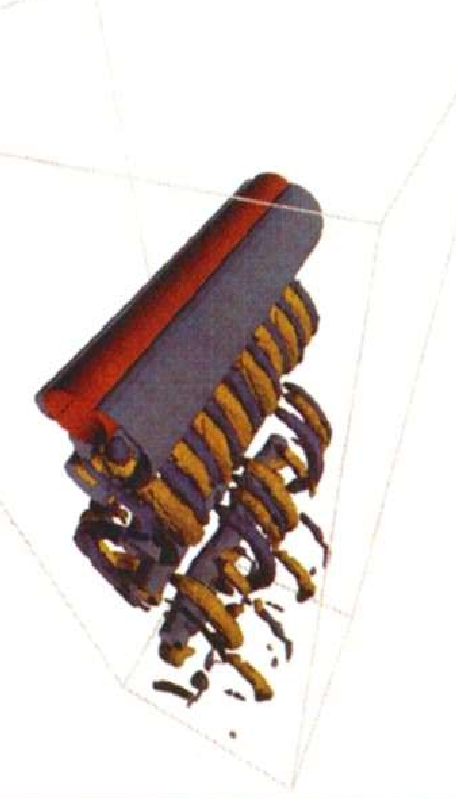
\includegraphics[angle=90,width=0.7\textwidth]{figs/modeB3D}
    \caption{Three-dimensional visualisation of mode B of Karman vortex shedding. Adapted from \citet{Thompson1994}.}
    \label{fig:modeB3D}
  \end{figure}
%%Chapter 2-8IE>>

% The Mathematica file used to compute the 20\% value below is in the file liftCoefficients67.50V2HHT.nb

%%Chapter 2-6IE<<
Noticeably, a lot of studies on streamwise vortex shedding discuss the process as a secondary process that is the offspring of the vortical structure that actually dominates the flow field - the spanwise Karman vortex. This trend in viewing streamwise vortex shedding as a secondary process is also found in \citet{Agbaglah2019}. In their numerical study of an isolated square and circular cylinder, they considered two Reynolds number, $\re = 205$ and $\re = 225$, and noted that the shedding frequencies of the two cylinders are quite similar. The Strouhal number St for the square cylinder is 0.152 and is 0.149 for the circular cylinder. Here, the Strouhal number St is defined as
%%Chapter 2-6IE>>

\begin{equation}
  \text{St} = \frac{f D}{U},
  \label{eq:stDef}
\end{equation}

\noindent where $f$, $D$ and $U$ are the characteristic frequency, characteristic length, and characteristic velocity of the flow. For a circular cylinder, $D$ becomes the diameter of the cylinder.

It is interesting to note that not only do they differ from each other only by two percent, but also that they differ by less than 20\% from the empirical equation (see, Eq. \ref{eq:karmanStrouhalNumber}) describing the shedding frequency of Karman vortices from a smooth circular cylinder \citep{Blevins1990}.

\begin{equation}
  \text{St}_{\text{Karman}} = 0.198 \left( 1 - \frac{19.7}{\text{Re}} \right)
  \label{eq:karmanStrouhalNumber}
\end{equation}

The fact that St for the square and circular cylinders of \citet{Agbaglah2019} differs less than 20\% of the value estimated using Eq. \ref{eq:karmanStrouhalNumber} indicates that the shedding process of streamwise vortex is overshadowed by Karman vortices, which are larger in scale. Perhaps this is an artefact of using an isolated cylinder, and as long as one uses a similar system, Karman vortex shedding will remain the primary process governing the flow.

More recent works on streamwise vortex shedding have shifted away from a simple isolated circular cylinder configuration to slightly more complex layouts, perhaps to recreate models that are more faithful to real engineering situations. For example, in \citet{Gibeau2018}, an elongated body is studied in the range $3.5 \times 10^{3} \leq \re \leq 7.0 \times 10^{3}$. Through this study, \citet{Gibeau2018} found that the average strength of the streamwise vortices in the upstream boundary layer is ten times smaller than in the wake. They also observed that the wavelength reaches between 0.7 and 0.8 of the elongated plate thickness, $h$.

 In another study, \citet{Gibeau2019} swapped the isolated circular cylinder for a blunt trailing edge body. This blunt trailing edge (BTE) body is made from a leading edge that is a 5:1 ellipse connected to a plate with thickness $h$. This experimental study in the range $2.6 \times 10^{2} \leq \re \leq 2.58 \times 10^{4}$, reveals that the rotational direction of the streamwise vortices are conserved during the shedding cycle, and their wavelength is close to mode B of \citet{Williamson1996a}.

Knowledge on the spatial distribution and key dimensions of streamwise vortices may be insufficient to highlight how one can exploit them to one's advantage. To exploit streamwise vortex shedding to fulfil engineering objectives, one needs insight on the effects of streamwise vortex shedding on the flow. This is demonstrated in the work by \citet{Rai2018}, in which the author published numerical results of flow around a flat plate with a circular trailing edge. The Reynolds number varies from $250 \leq \re \leq 10000$. \citet{Rai2018} discovered that streamwise vortices are responsible for generating steep spanwise velocity gradients that affect the strength of the dominant vortical structure of the flow, i.e. the Karman vortex. The author also found that fluctuations in the streamwise velocity within the boundary layer leads to variation in the shedding period of the dominant Karman vortex. Finally, streamwise vortex shedding is observed to affect the shedding frequency of the spanwise Karman vortices through the speed of their streaks in the boundary layer.

In an evaluation of a passive method to control flow around a circular cylinder, \citet{Lin2018} inserted the cylinder inside a conical shroud and assessed its effect on the vortical structures shed around it. Their conical shroud is shown in Fig. \ref{fig:conicalShroud}. A very low $\re = 100$ was chosen to keep the flow as two-dimensional as possible.

\begin{figure}[!h]
  \centering
  \hspace{1cm} 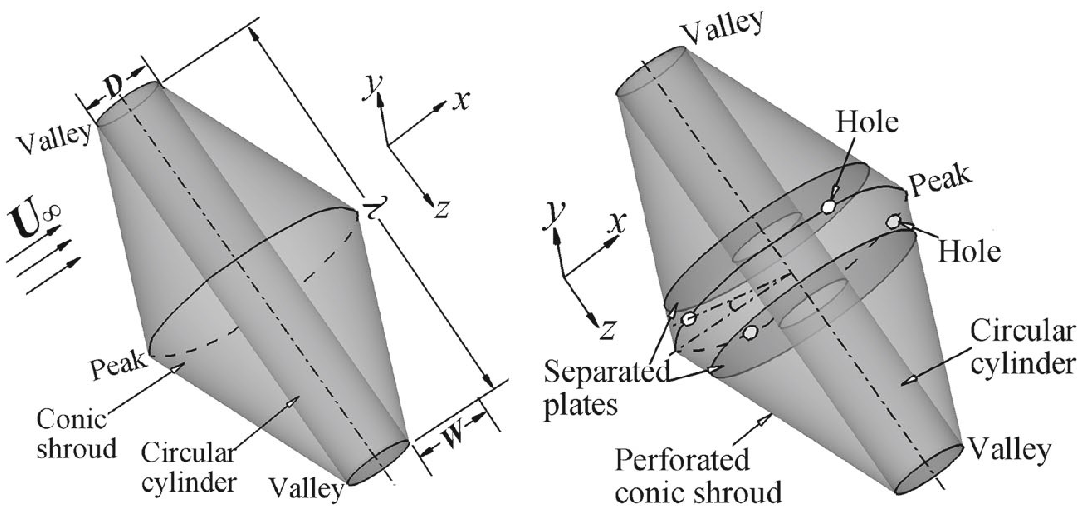
\includegraphics[width=0.7\textwidth]{figs/conicalShroud}
    \caption{The conical shroud used by \citet{Lin2018}.}
    \label{fig:conicalShroud}
  \end{figure}

  \noindent \citet{Lin2018} tested two types of conical shroud. One shroud is with perforations of varying diameter and placement angle along the peak of the cone, and the other without. The authors also varied the wavelength and outer diameter of the conical shroud. By doing so, the study essentially discovered a method to prevent the energising of Karman vortex when the disturbance brought about by the conical shroud is large enough. Energy from the freestream is redirected away from Karman vortices, to form strong $\Omega$-shaped vortices in the neighbourhood of the conical valley, some examples of which are given in Fig. \ref{fig:omegaVortices}. The name $\Omega$-vortex comes from the fact that the vortices being shed downstream the cylinder resembles the uppercase Greek letter ``omega'' ($\Omega$), when viewed from the direction of $+y$ of their coordinate system.

  \begin{figure}[!h]
    \centering
    \begin{subfigure}[h]{0.45\textwidth}
      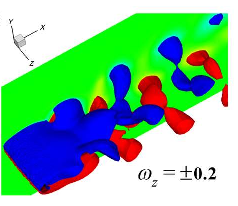
\includegraphics[width=\textwidth]{figs/omegaVortexB}
      \caption{Omega vortex at $t=470$ s.}
      \label{fig:omegaVortexB}
    \end{subfigure}

    \begin{subfigure}[h]{0.45\textwidth}
      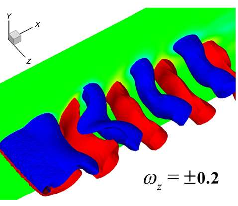
\includegraphics[width=\textwidth]{figs/omegaVortexC}
      \caption{Omega vortex at $t=500$ s.}
      \label{fig:omegaVortexC}
    \end{subfigure}

    \begin{subfigure}[h]{0.45\textwidth}
      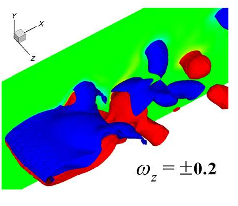
\includegraphics[width=\textwidth]{figs/omegaVortexA}
      \caption{Omega vortex at $t=900$ s.}
      \label{fig:omegaVortexA}
    \end{subfigure}

    \caption{Some examples of the $\Omega$-vortices from \citet{Lin2018}, taken at different times of the simulation.} \label{fig:omegaVortices}
  \end{figure}


  This results in partial to full suppression of Karman vortex shedding. The ability to refocus energy to a vortical structure of choice is indispensable, especially to engineers who may either want to minimise cyclic force acting on a structure, or maximise it to improve vibration energy harvesting potential of the structure.

Other examples of energy redirection can be found in \citet{Zhang2016} and \citet{Zhang2019}. In these studies, the authors examined two methods to control Karman vortex shedding from a model bridge. The first method in \citet{Zhang2016} employs suction on the bottom of the bridge to disrupt the homogeneity of the Karman vortex along the span of the bridge. When suction is applied, streamwise vortex - which is considered a secondary process by the authors - becomes energised. The energised streamwise vortex then destabilises the primary vortical structure - the Karman vortex - hence reducing the net force resulting from it.

Providing suction on the bottom of the bridge is an active flow control method. This is because an active supply of energy is required to power the suction from the designated holes. As an alternative, \citet{Zhang2019} proposed using vortex generators affixed similarly to the bottom of the bridge, and evaluates the degree to which a similar result can be achieved. In the final analysis, they demonstrated that the disruption of Karman vortex homogeneity is possible through the use of vortex generators. However, they did not specify quantitatively how much weaker does the Karman vortices get in expense of stronger streamwise vortices.

Attachment of a plate \citep{Gibeau2019} or placement of the cylindrical object inside a conical casing \citep{Lin2018} - even the deployment of vortex generators on the surface of the cylinder \citep{Zhang2019} - are all methods of flow control that add another layer of complexity to the cylindrical object. In situations where an engineer seeks to retrofit a flow control method to existing systems with cylindrical objects, direct modification of the cylinder can be difficult and downright undesirable. What if there exists an accessible flow control method that requires only a minimum amount of effort from the end used to install, but is still powerful enough to significantly alter the dominant vortical structures of the flow? The deployment of another cylindrical object downstream the main cylinder seems to be a promising technique.

Flow control using a secondary cylinder placed downstream the main cylinder dates back nearly three decades. Originally, the authors investigating it \citep{Shirakashi1989} is focussed on reducing the magnitude of cyclic forces acting on an isolated circular cylinder system. They placed a secondary circular cylinder downstream the original circular cylinder and explored how, among others, \rms{} lift coefficient of the original cylinder varies as the gap between the original and secondary cylinders are varied. The secondary cylinder is placed downstream the original in a way such that the axes are perpendicular to each other, creating a cruciform. In doing so, they discovered that while the \rms{} of lift coefficient can be reduced as the downstream cylinder is brought closer to the original one, when the normalised gap between two cylinders $g/D$ is $< 0.25$ the lift coefficient rises again and peaks close to $\approx 0.7$ before dropping off again as $g/D \to 0$. This is a significant finding in that it demonstrates how the flow around an existing isolated cylinder system can be altered in hindsight by simply forming a cruciform structure with another cylinder.

The dominant vortical structure in such a cruciform when $0 < g/D < 0.5$ is dominated by a pair of streamwise vortices, shed alternately from the top and bottom of the primary cylinder \citep{Koide2017}. Two types of streamwise vortices are observed, the necklace vortex when $0.25 < g/D < 0.5$, and the trailing vortex when $0 < g/D < 0.25$. This is illustrated in Fig. \ref{fig:streamwiseFigure}. Although both types of vortices form close to the cruciform juncture, the necklace vortex dominates a region that is closer to the juncture than the trailing vortex \citep{Takahashi1999}, which forms a little further away from the juncture. The streamwise vortex pair that forms due to the cruciform does not seem to be secondary to the Karman vortex that is also shed from the upstream cylinder. Instead, the streamwise vortices seem to have its own mechanics which is independent from the cycle of Karman vortex shedding.

\begin{figure}[!h]
  \centering
  \begin{subfigure}[h]{0.45\textwidth}
    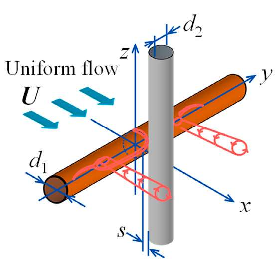
\includegraphics[width=\textwidth]{figs/streamwiseTrailing}
    \caption{Trailing vortex, $0 < g/D < 0.25$.}
    \label{fig:streamTrail}
  \end{subfigure}
  \hspace{1cm}
  \begin{subfigure}[h]{0.45\textwidth}
    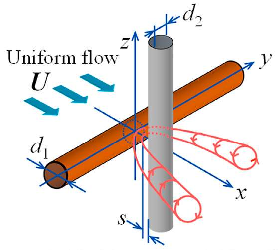
\includegraphics[width=\textwidth]{figs/streamwiseNecklace}
    \caption{Necklace vortex, $0.25 < g/D < 0.5$.}
    \label{fig:streamNecklace}
  \end{subfigure}

  \caption{A schematic of streamwise vortex shedding, adapted from \citet{Hemsuwan2018a}.} \label{fig:streamwiseFigure}
\end{figure}


One obvious example is the deference to Eq. \ref{eq:karmanStrouhalNumber}. Streamwise vortices such as those discussed earlier \citep{Zhang2016,Rai2018,Agbaglah2019,Zhang2019} develop as three-dimensional instabilities of Karman vortex shedding, and as such, have a base shedding frequency that loosely obeys Eq. \ref{eq:karmanStrouhalNumber}. However, streamwise vortices in \citet{Takahashi1999}, and even in \citet{Shirakashi2001} and \citet{Bae2001} do not. Streamwise vortices from these studies are shed at an increasing St as Re is increased within the region $\re < 10000$. When $\re > 10000$, St for the streamwise vortex becomes more or less constant with $\st \approx 0.04$ for the necklace vortex and nearly twice that value for the trailing vortex.

Domination of the cruciform flow field by the streamwise vortex pair does not imply that the Karman vortex completely disappears from the experimental domain. This is demonstrated in \citet{Koide2006} and \citet{Kato2006}. According to the frequency spectra of the upstream cylinder vibration, the Karman shedding frequency still exist in the system, only far smaller in magnitude compared to the amplitude attained by the streamwise vortex structures. The flow field is thus dominated by the streamwise vortex pair close to the cruciform juncture, while the influence of the Karman vortex only grows as one moves towards the ends of the upstream cylinder. This begs the question whether the streamwise vortex-dominant flow is simply a consequence of two circular cylinders at right angles to each other - placed some distance away from each other - or is it something universal to cruciforms structures?

To answer this, \citet{Kato2007} and \citet{Nguyen2010} tested several variations of the cruciform, to see whether a similar occurrance of streamwise vortex shedding can be observed. For example, \citet{Kato2007} swapped the downstream circular cylinder with a strip plate, and observed that similar streamwise vortices do appear in the flow. They are shed at very similar values of St as the two-cylinder cruciform, but the frequency spectra of velocity fluctuations revealed a noisier pattern with less discernable peaks compared to the frequency spectra computed from a two-cylinder cruciform. More recent flow visualisations suggest that the noisier pattern is due to an increased turbulence level in the flow as streamwise vortices are produced from the circular cylinder-strip plate system \citep{Koide2017}. Streamwise vortices produced from the two-cylinder system however, is less turbulent and thus one finds less distortion in the vortical structures compared to the circular cylinder-strip plate cruciform.

Distortion of the vortical structures discussed in \citet{Kato2007} and \citet{Koide2017} are self-induced: the result of an increasing level of turbulence in the flow. An increased level of turbulence is something that is internal to the flow being considered. It remains to be seen whether external factors such as the type of medium used as the ambient fluid, or configuration of the experimental rig can affect the shedding behaviour of the streamwise vortices. The work by \citet{Nguyen2010} partially answers this question. In their study, the two-circular cylinder cruciform is tested under various settings. They tested the system in wind and water tunnels of various sizes and ascribing different dimensions to the cruciform. The dimensions \citet{Nguyen2010} vary in their experiments are the circular cylinder diameter, cylinder length and aspect ratio. At the end of their study, \citet{Nguyen2010} concluded that nearly all major characteristics of streamwise vortex shedding are observed under the various test conditions. There are, however, some discrepancies namely reduction by 30\% to 50\% of streamwise vortex shedding St in the largest wind tunnel, and the vanishing of the necklace vortex in the water tunnel as $\re > 22400$.

Clearly, streamwise vortex shedding that results from the deployment of a cruciform structure is robust and induces as much force on the upstream cylinder as Karman vortex shedding on an isolated cylinder, if not more. This makes the cruciform structure a good oscillator candidate for the purpose of converting energy from the free stream in to vibration energy. In the next section, the author reviews the recent developments in VIV and discusses how a cruciform oscillator ties into the overall work done to induce a larger, but predictable vibration from fluid flows, including that which depends on Karman vortex.

\section{Vortex-induced Vibration of a Cylinder} \label{sec:cylinderVIV}
In this section, the thesis looks into the literature on vibration that is induced from the vortex being shed from a cylinder whose axis is perpendicular to the direction of the freestream. In particular, the following sections are going to collect and synthesise information on the transverse oscillation response of the cylinder and summarise how it evolves with respect to parameters such as the Reynolds number and reduced velocity.

\subsection{Single Cylinder Oscillator Unit} \label{ssec:singleCylinderOscillator}
Since Karman vortex shedding has been demonstrated to produce alternating lift and drag on an isolated cylinder system, replacing motion constraints with elastic supports allows oscillatory motion to take place. Typically, the oscillation is constrained to a one-dimensional transverse motion against the direction of the free stream. Following the success of \citet{Raghavan2007a} and  \citet{Bernitsas2008b} in achieving a high amplitude response from an isolated circular cylinder oscillator, experimental studies for such an oscillator are increasingly done in the $2 - 4 \times 10^{4} \leq \re \leq 1 - 2 \times 10^{5}$ range.

Numerical studies provide a non-intrusive method to collect high-resolution data on flow quantities. Following the trend in experimental studies of VIV, an increasing number of works have been pushing through the $\re \sim O(10^{5})$ barrier, and collect time-resolved flow quantities that lay the groundwork for advancing VIV flow theory. Additionally, if one is able to develop a working numerical model of VIV at a particular range of Re that is in good agreement with experimental findings, scholars can then use that model to automate the variation of parameters. This automation enables efficient exploration of the parameter space of interest and rapid product prototyping.

However, for numerical works to accurately depict what is going on in the flow at $\re \sim O(10^{5})$, investigators need to abandon one of the most commonly made assumption to simplify the KVIV phenomenon: that the flow is two-dimensionally reducible. Reducing KVIV to a two-dimensional domain greatly reduces computational requirements and allows the researcher to focus the computational effort on resolving the shear layer of the cylinder and the near-wake region. However, three-dimensional effects exists throughout the flow field as soon as $\re > 150$, and an accurate representation of KVIV necessitates taking these effects into account.

\citet{Kinaci2016} proposed a tip-flow correction factor to reduce deviation of a two-dimensional CFD simulation from experimental results. The tip-flow correction factor is computed from three-dimensional simulation of flow around a cylinder within the Re range of interest, in essence providing the reader with a new ``effective length'' of the cylinder. The success of this method is however quite limited as it only scales the lift magnitude from a two-dimensional simulation, but not the phase lag between the lift and cylinder displacement. This means that to conduct a meaningful study of KVIV in the TrSL3 regime ($2 - 4 \times 10^{4} \leq \re \leq 1 - 2 \times 10^{5}$) one must rely on experiments and three-dimensional simulations to explore the bulk of parameter space.

One of the recent developments in the control of KVIV is by affixing passive turbulent stimulations on the surface of the cylinder. For example, \citet{Park2016} deploys surface roughness on the cylinder and observed their effect on KVIV. They identified several location on the cylinder that produces weak to high reduction in the amplitude response. They reasoned that this is due to the reduction of vorticity in the shear layer that forestalls vortex roll-up, hence trim the vibration amplitude by at least a factor of three. This forestalling of vortex shows that surface roughness on the scale of the shear layer thickness can alter the vorticity and thus the lift production process of the cylinder.

The altering of vorticity in the shear layer is also what enables the bridging of KVIV and galloping in single cylinder systems with surface roughness. At low angles of attachment of the roughness strip \citep{Park2013}, the flow separates at the strip upstream but reattaches further downstream the cylinder surface. At high angles of attachement, there is not enough distance along the cylinder surface for the separated flow to reattach, hence vorticity cancellation between Karman vortices shed from the top and bottom of the cylinder becomes comparatively more aggressive. The absence of this aggressive cancellation of spanwise vorticity is the reason why placement of the roughness strip is able to, in contrast to \citet{Bernitsas2008c} and \citet{Park2016}, enhance KVIV and improve the amplitude response of the single cylinder oscillator.

In Section \ref{ssec:svShedding}, this work discussed how the cruciform system has its origin as a simple method that can be retrofitted to an existing single cylinder oscillator unit to control Karman vortex shedding. As such, the effect of the downstream cylinder/strip plate is targeted towards the upstream cylinder and not itself. However, within the last five years, the VIV research community has increasingly realised that there is no reason for the conversion of energy from the free stream into vibration to strictly be a one-stage process. Excess energy that is not eludes capture by a single cylinder should simply be recovered with another cylinder downstream.

Bearing this in mind, \citet{Ding2017} investigated the system response of a two-circular cylinder system, one in front of the other and with their axes parallel to each other. This system is illustrated in Fig. \ref{fig:twoCylinderSystem}.

\begin{figure}[!h]
  \centering
  \hspace{1cm} 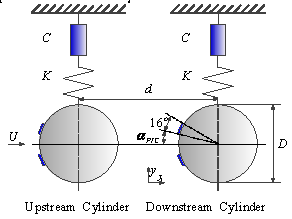
\includegraphics[width=0.65\textwidth]{figs/twoCylinderOscillator}
  \caption{The two-circular cylinder system of \citet{Ding2017}.}
  \label{fig:twoCylinderSystem}
\end{figure}

\noindent Then, they measured the amplitude/frequency responses of the system and observed the following, compared against a single cylinder system with passive turbulence control (PTC). The amplitude response of the upstream cylinder seems to improve in this serial arrangement of cylinders, and they experience only a small influence from centre-to-centre distance variation. On the other hand, the downstream cylinder experiences a reduction in the amplitude response compared to a single cylinder system and is more sensitive to the centre-to-centre distance between the two cylinders. The reduced amplitude response of the downstream cylinder is the result of the acquisition of downstream cylinder vorticity by the upstream cylinder in proximity. Proximity between the two cylinders determine how much downstream cylinder vorticity is carried away by the upstream vortex, and this reduces the net lift acting on the downstream cylinder. The reduction of lift finally results in the reduction of downstream vibration amplitude.

There is however, a countermeasure to improve the amplitude response of the downstream cylinder. The improvement is achieved by imposing a smaller damping on the downstream cylinder \citep{Xu2017}. When \citet{Xu2017} reduced damping for the downstream cylinder, the amplitude response of the downstream cylinder becomes more similar to the amplitude response of the upsteram cylinder. Nevertheless, because harnessed power is proportional to damping - specifically damping in the mechanical to electrical power converter - a reduced total damping just to achieve a higher amplitude vibration is simply contrary to the engineer's main objective of energy harvesting \citet{Bernitsas2009}.

Spacing between the two cylinders play an important role in obtaining maximum vibration amplitude from both the upstream and downstream cylinders. This much is already known from the works of \citet{Park2016} and \citet{Ding2017}. However, recently, \citet{Yuan2020} utilised the Hilbert transform on the cylinder displacement time series of both upstream and downstream cylinders. In doing so, they identified five major responses of the two-cylinder oscillator that depends primarily on the centre-to-centre distance between the two cylinders, and secondarily on other parameters such as spring coefficient and total damping.

The use of Hilbert transform enabled \citet{Yuan2020} to compute instantaneous frequency and phase lag between the upstream and downstream cylinders and identified the five major response regimes of the system. Although \citet{Yuan2020} have essentially demonstrated the utility of Hilbert transform in analysing complex and interdependent systems of vibration, the signals they analysed are for the most part monocomponent signals with more or less a symmtetrical signal envelope. For signals that lack these features, the pre-processing step of empirical mode decomposition (EMD) or ensemble empirircal mode decomposition (EEMD) is necessary to produce meaningful physical results \citep{Chen2019}.

\subsection{Cruciform Oscillator Unit}
Streamwise vortex-induced vibration (SVIV) is a type of vortex-induced vibration (VIV) driven by vortical structures whose vorticity vector points in the direction of the free stream. In its early days, the cruciform oscillator is nothing but two circular cylinders perpendicular to each other, overlapping at their midpoints \citep{Zdravkovich1985}. A cruciform oscillator unit, as shown in Fig. \ref{fig:twoCrossingCylinders}, derives its vibration from the streamwise vortex pairs discussed in Section \ref{ssec:svShedding}.

\begin{figure}[!h]
  \centering
  \hspace{1cm} 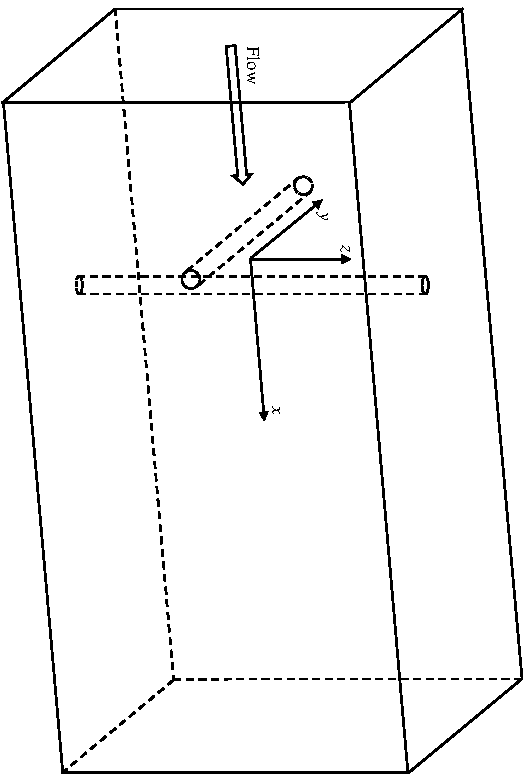
\includegraphics[angle=90,width=0.7\textwidth]{figs/twoCrossingCylinders}
  \caption{The two-circular cylinder cruciform of \citet{Zhao2018a}.}
  \label{fig:twoCrossingCylinders}
\end{figure}

\noindent When the upstream cylinder as shown in Fig. \ref{fig:twoCrossingCylinders} is no longer fixed and is supported elastically through some form of spring, the shedding of streamwise vortices causes SVIV to occur. Investigators observed the upstream cylinder acquiring significant vibrations in the order of $O(10^{-1}D)$, as the reduced velocity of the flow $\ured$ exceeds 14. Notice that there is a gap between the upstream and downstream cylinders.

Interestingly, however, the latest published research on a zero-gap circular cylinder cruciform system between $300 \le \re \le 1800$ revealed that no streamwise vortex cell are formed and shed from the structure \citep{Tang2021}. This work by \citet{Tang2021} was a numerical one, employing large eddy simulation (LES) with the dynamic $k$-equation subgrid-scale (DKSGS) model. Even the time history of the drag and lift coefficients did not show significant levels of periodicity, similar to those found in \citet{Deng2007}, although they both simulate flow in the same Reynolds number magnitude of $O(10^{2})$. In fact, \citet{Deng2007} simulated the flow around a circular cylinder cruciform at a much lower $\re$ and still were able to observe the formation of the streamwise vortex cells and their footprint, manifesting themselves as the periodic oscillation of the drag and lift coefficients. What can be deduced from this is the gap between two cylinders forming a cruciform is essential for the formation of streamwise vortices and ultimately the vibration induced by it.

In their study of the two-circular cylinder cruciform, \citet{Shirakashi2001} observed the vibration of the upstream cylinder hitting the top boundary of the wind tunnel between $20.5 \leq \ured \leq 35.9$. The height of the wind tunnel in \citet{Shirakashi2001} is 320 mm and the diameter of both upstream and downstream cylinders are 26 mm. The fact that the reported vibration amplitude reaches the top extent of the wind tunnel means that it is able to achieve at least $(\SI{320}{\milli\metre}/2)/\SI{26}{\milli\metre} = 6D$ within $20.5 \leq \ured \leq 35.9$. This alone is far bigger than any of the amplitude attained by the single cylinder oscillator units reviewed in Section \ref{ssec:singleCylinderOscillator}. However, there seems to be a finite range within which the cruciform oscillator is able to sustain this high amplitude response, which is approximately 15 units of $\ured$. Past this, the amplitude of the cylinder drops to about $0.1D$ and stayed there up to the maximum $\ured$ tested. In contrast, single cylinder oscillators of Section \ref{ssec:singleCylinderOscillator} is able to sustain its vibration through galloping for seemingly an infinite range of $\ured$.

More recent iterations of the system such as in \citet{Koide2007} and \citet{Kato2007} employs a thin, rectangular plate of width $w = D$ in place of the fixed downstream cylinder, and showed that the region of high-amplitude vibrations of the system is enlarged from 15 units of $\ured$ for a two-circular cylinder cruciform to approximately 40 units of $\ured$ for the circular cylinder-strip plate oscillator studied in \citet{Koide2007}. Nevertheless, the shortcoming of this configuration is a lower amplitude of vibration, which attains only a maximum of close to $\yrms = 0.35$. The vibration amplitude in \citet{Koide2007} and \citet{Kato2007} is given as the \rms{} of nondimensionalised vibration amplitude $\yrms = y_{\text{RMS}}/D$. Here, $y$ denotes the coordinate pointing in the transverse direction of the flow, i.e. the direction of cylinder vibration. The effect of circular cylinder-strip plate gap $g/D$ on $\yrms$ was also examined, and the results were consistent with the trend of high lift generation discussed in Section \ref{ssec:svShedding}: $\yrms$ jumps to a high-amplitude regime as $g/D$ is decreased to $< 0.5$, especially when $g/D < 0.25$.

However, at $G = g/D = 0.16$, researchers have found that the circular cylinder-strip plate oscillator managed to sustain its vibration over a very large range of $\ured$. In relative terms, the vibration of this variant of the cruciform is sustained over a range of $\ured$ 15 times the width observed in an isolated, smooth circular cylinder oscillator of similar diameter. This has been observed in \citet{Koide2009} and \citet{Koide2013}. The reason behind this is the vortical structure driving the vibrations: vibration of the cruciform is driven by a pair of counter-rotating streamwise vortex shed a short distance from the cruciform juncture (refer Fig. \ref{fig:oscillatorSchematic}), while vibration of the isolated, smooth circular cylinder is driven by Karman vortices shed alternately from the top and bottom surface of the cylinder.

\begin{figure}[!h]
  \centering
  \hspace{1cm} 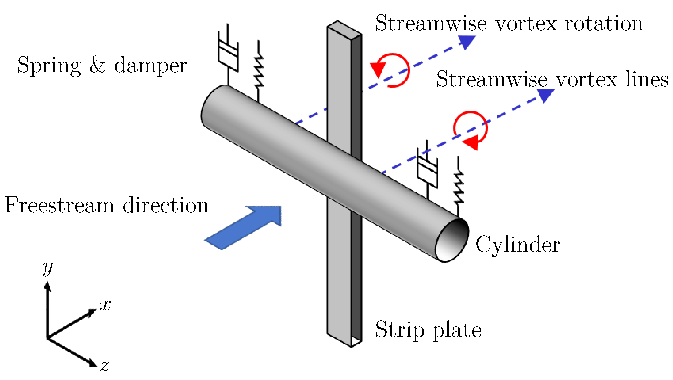
\includegraphics[width=0.7\textwidth]{figs/oscillatorSchematic}
  \caption{Schematic of the base configuration of the oscillator system used in this study, i.e. the pure cruciform.}
  \label{fig:oscillatorSchematic}
\end{figure}

The upside of this discovery is the fact that this wide synchronisation range is due to vortex shedding i.e., vortex-induced vibration (VIV) instead of galloping, as in \citet{Sun2019b}, \citet{Xu2019} and \citet{Ding2019}, as VIV-based energy harvesters of similar scale operate at higher efficiencies compared to galloping-based ones. \citet{Sun2016} and \citet{Ma2016} also obtained a similar result.

In their study, \citet{Deng2007} examined the flow field of a twin circular cylinder cruciform using computational fluid dynamics (CFD). Their domain stretches  $28D$  in the streamwise direction,  $16D$  in the transverse direction and  $12D$  in the spanwise direction. They studied an Re range yet another order of magnitude smaller than that studied by \citet{Koide2017}, possibly to get an even clearer visualisation of the vortical structures with less turbulence, and to ease computational requisites. At a fixed  $\re = 150$ , streamwise vortices form even at a gap ratio of $2$. This result differs quite strikingly from \citet{Koide2006} and \citet{Koide2007}, conducted at an Re twice the order of magnitude of \citet{Deng2007}, an indication that the minimum gap ratio needed for the onset of streamwise varies with respect to Re.

They also observed that when the gap ratio $G$, which they denote as  $L/D$  in their paper, increases from 3 to 4, the maximum amplitude of the lift coefficient increases by almost threefold. This can be attributed quite easily to the current vortex pair shed by the upstream cylinder. The downstream cylinder immediately disturbs the pair shed from the upstream cylinder when  $G=3$. The lift coefficient increases by about a factor of 3 when this immediate disturbance diminishes at  $G=4$. The visualisation of three-dimensional (3D) vorticity isocontours enables the present work to quickly establish this link vis-\`{a}-vis the lift coefficient signal. The authors use of CFD made this possible.

A similar study in the order of magnitude $\re \sim O \left( 10^{2} \right)$ by \citet{Zhao2018a} particularly highlighted the immense utility of CFD as a tool to research SVIV or flow around a cruciform in general. They computed the sectional lift coefficient along the upstream cylinder, and the time history of this sectional lift coefficient revealed two different modes of vortex shedding, namely, parallel and K-shaped. They also paid attention to the local flow patterns that vary along the length of the upstream cylinder such as the trailing vortex flow, necklace vortex flow and flow in the small gap (denoted as SG flow). The discontinuities in the phase angle of the sectional lift coefficient along the upstream cylinder seems to suggest the inadequateness of attributing the lift coefficient to streamwise vortex shedding alone, particularly when Karman vortex streamlines were also observed some distance away from the junction of the cruciform.

\citet{Shirakashi1989} also made a similar observation in their experimental work. These observations lead the present author to hypothesise that the lift signal is more appropriately viewed as the streamwise and Karman vortex-induced composite lift signal. The present work, nevertheless, could neither find studies that took this viewpoint, nor work out its consequence on power generation. It is worth mentioning that there was a recent development in this field of study, which investigated a square cylinder and a square plate downstream of it \citep{Mohamed2021}. This is essentially a variant of the canonical cruciform structure where the upstream circular cylinder is swapped for a square one, and the downstream strip plate is shortened to the same height of the upstream square cylnder. From all the experimental conditions tested, \citet{Mohamed2021} found only one setup that enhances the KVIV amplitude of the system, which is when the side ratio and gap ratio of the system is $(B/D, g/D) = (1.0, 1.17)$, while other setups cut down the KVIV amplitude by a factor of two. Galloping however, receives a boost in the root-mean-square amplitude at $(B/D, g/D) = (1.2, 1.15)$ and $(1.4, 1.15)$, making this setup a galloping-oriented oscillator and ultimately, energy harvester.

\section{Energy Harvesting from a Vibrating Cylinder} \label{sec:energyHarvesting}
The field of energy harvesting has witnessed exponential growth in the past two decades, particularly those which are based on alternating lift mechanisms. Following the same method used in the previous Section \ref{sec:cylinderVIV}, the author reviews the progress in the single cylinder energy harvesting unit first, followed by the recent advances in the cruciform systems.

\subsection{Single Cylinder System} \label{ssec:singleCylinderHarvester}
Recent advances in energy harvesting from a single cylinder system builds upon the body of work done on single cylinder oscillators. One of the overarching themes in power output improvement from a single cylinder system is the operating range of Re. Ever since the work done by \citet{Bernitsas2008a} and \citet{Bernitsas2009}, prototyping studies have planted their foot firmly in the high lift regime of TrSL3. In doing so, studies such as \citet{Ding2019} and \citet{Park2017} managed to demonstrate an amplitude response with an upper branch sustained over a wider range of $\ured$ compared to amplitude responses of single cylinder systems in TrSL1 or TrSL2. A higher vibration amplitude will elicit a higher harnessed power from the harvester.

Here, TrSL1, TrSL2 or TrSL3 refers to the classification system in \citet{Zdravkovich1997} to characterise the flow around a smooth circular cylinder. The classification system uses abbreviations of the flow description as labels for different flow behaviours. For example, the flow around the circular cylinder undergoes a number of transitions in the shear layer between $350 - 500 \leq \re \leq 1 \times 10^{5} - 2 \times 10^{5}$. The \underline{\textbf{first}} \underline{\textbf{tr}}ansition in the \underline{\textbf{s}}hear \underline{\textbf{l}}ayer, occurring between $350 - 500 \leq \re \leq 1 \times 10^{3} \times 2 \times 10^{3}$, is the development of transition waves. \citet{Zdravkovich1997} labeled this regime as TrSL1, formed by joining the abbreviations of ``transition'', ``shear'', ``layer'', and the numerical equivalent of ``first'', which is the number one (1). Similarly, the second transition in the shear layer occurring between $1 \times 10^{3} - 2 \times 10^{3} \leq \re \leq 2 \times 10^{4} - 4 \times 10^{4}$, which is the formation of free vortices, is labeled as TrSL2. The shear layer becomes fully turbulent between $2 \times 10^{4} - 4 \times 10^{4} \leq \re \leq 1 \times 10^{5} - 2 \times 10^{5}$. This regime is thus labeled TrSL3. 

Now with the single cylinder system firmly planted in the TrSL3 regime, researchers worked to push the single cylinder harvesting system even further by tweaking its mechanical parameters. For example, \citet{Sun2018} and \citet{Ma2018} used as the restorative force, i.e. springs, of the nonlinear variant. This is achieved by connecting the vibrating cylinder not to a physical spring and damper, but instead to a computer-controlled motor, for example as shown in Fig. \ref{fig:vckSystemModel}. This motor can be programmed to act like a spring and damper, each with its own coefficients $k$ and $c$. So instead of modelling the spring linearly as

\begin{figure}[!h]
  \centering
  \hspace{1cm} 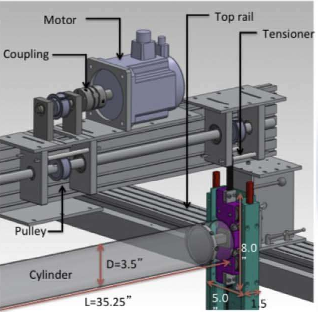
\includegraphics[width=0.7\textwidth]{figs/vckSystemModel}
  \caption{A three-dimensional drawing of the system to control the mechanical parameters of the system. Adapted from \citet{Ma2018}.}
  \label{fig:vckSystemModel}
\end{figure}


\begin{equation}
  F(t) = k x(t),
  \label{eq:linearSpring}
\end{equation}

\noindent where $F(t)$ is the restorative force, $k$ the spring coefficient and $x(t)$ the displacement of the object fixed to the end of the spring, they experimented with $F(t)$ that is given as a cubic function and an $F(t)$ that is given as a piecewise linear function. The cubic spring of Eq. \ref{eq:cubicSpring}

\begin{equation}
  F(t) = k y(t) + k y(t)^{3},
  \label{eq:cubicSpring}
\end{equation}

\noindent is found to significantly improve energy harvesting in all branches of amplitude response. Most significantly, however, is the improvement in the transition from VIV lower branch to galloping branch. In systems with a linear restorative force, the VIV lower branch is out of sync with the lift and also vortex shedding. This causes the net power harnessed in this regime to drop up to a factor of three, compared to the power harnessed in the upper branch of VIV \citep{Sun2018,Ma2018}. In contrast, when a cubic restorative force is applied to the system, energy harvesting improves by up to 78\% during the transition from lower branch to galloping. Furthermore, once the system enters the galloping regime, the cubic restorative force improves energy harvesting up to 12\%. In fact, the only branch where the original linear restorative force outperforms the cubic spring system in terms of energy harvesting is the upper branch.

Differently, a piecewise linear spring such as in Eq. \ref{eq:piecewiseLinearSpring}, in essence enables switching of system stiffness and natural frequency according to the cylinder displacement.

%%Chapter 2-9IE<<
\begin{equation}
  F(t)=\begin{cases}
    k_{1} y(t),                              & \text{if $|y(t)| \leq y_{0}$}\\
    k_{1} y(t) y_{0} + k_{2} (y(t) - y_{0}), & \text{if $|y(t)| > y_{0}$}.
  \end{cases}
  \label{eq:piecewiseLinearSpring}
\end{equation}
%%Chapter 2-9IE>>

\noindent Through this modification, the system is able to automatically switch to a lower stiffness when the lift acting on the cylinder is small, and to a higher stiffness otherwise. A higher stiffness results in a higher system natural frequency. Consequently, when the system is in sync with the alternating lift and vortex shedding, thus producing a large vibration amplitude, the frequency of vibration also switches to a larger value. This switch to a larger value is valuable as the harnessed power from such a system is proportional to the square of its angular frequency \citep{Ma2018}.

Apart from this, the piecewise linear spring is able to harness energy even when $\re < 25000$, which is lower than the usual linear spring system of Eq. \ref{eq:linearSpring} \citep{Sun2016}. In terms of damping, although it is proportional to the net harnessed power \citep{Ma2018}, there is a trade-off with the size of the stall zone during transition from VIV to galloping. The width of the stall zone increases with increasing system damping, and this reduces the system's range of operability. Furthermore, in a single cylinder system with a linear spring, simply increasing the damping reduces the maximum vibration amplitude.

Interestingly, this suppression effect on vibration amplitude due to increased damping can be kept in check when one uses the in-tandem arrangement of cylinders. The in-tandem system is similar to that discussed in Section \ref{ssec:singleCylinderOscillator}, and \citet{Sun2019b} observed that the amplitude reduction is not as severe in the in-tandem system compared to the single cylinder unit. This highlights the potential of exploiting the synergy between the two cylinders to counter vibration amplitude reduction that is otherwise striking, provided that the two cylinders are optimally spaced. The results also brought attention to the concept of synergy between single cylinder oscillators in order to harness more energy from the flow.

\citet{Kim2016} took the idea of synergy and investigated a four-cylinder system for energy harvesting. Overall, what they found out was the net energy harvested by the four-cylinder system can exceed the total energy harvested by four isolated cylinder, provided that the four-cylinder system adhere to the optimised system parameters of centre-to-centre cylinder spacing, mass ratio, spring stiffness and damping. They also postulated an energy harvesting unit that consists of stacked arrays of single cylinder oscillators, thus maximising the footprint of the unit and increase power-to-volume density of the system. In summary, \citet{Kim2016} highlighted the need for the research community to widen their perspective and pay greater attention to multi-component energy harvesting systems as there is a high chance that one can discover practical arrangement of the components that increases the net harnessed energy. The next subsection explores one such system: the pure cruciform energy harvester.

\subsection{Pure Cruciform System} \label{ssec:pureCruciformHarvester}
A pure cruciform \citep{Zou2021} system  is an example of a multicomponent energy harvester where the presence of the downstream plate perpendicular to the upstream cylinder alters the flow such that the vibration response of the upstream cylinder becomes different from the single cylinder oscillator. In such an energy harvesting system, there exists two vortical structures regulating the flow around the cruciform: the Karman and streamwise vortices. However, as the present study discussed in Section \ref{ssec:svShedding}, only the shedding of streamwise vortex is able to synchronise with the alternating lift and cylinder displacement, thus producing a cylinder response fit for energy harvesting.

An example the cruciform system is given in Fig. \ref{fig:oscillatorSchematic}. In broad terms, the literature on SVIV-based energy harvesting from pure cruciform oscillators are either one of these two categories: studies that investigate how the mass ratio, spring stiffness and damping affect the system response, and studies that put into the spotlight the details of flow that regulates the lift acting on the elastically supported cylinder, hence its amplitude/frequency response, which directly influences the system's energy harvesting capabilities.

For example, \citet{Koide2009} investigated such an energy harvesting system by varying a number of parameters defining the vibration-to-electrical energy converter. The energy converter schematic is given in Fig. \ref{fig:coilGenerator}.

\begin{figure}[!h]
  \centering
  \hspace{1cm} 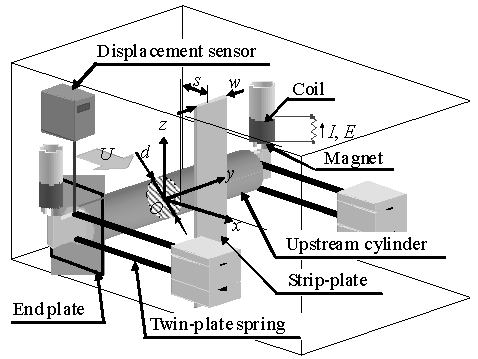
\includegraphics[width=0.7\textwidth]{figs/coilGenerator}
  \caption{The vibration-to-electrical energy converter of \citet{Koide2009}.}
  \label{fig:coilGenerator}
\end{figure}

\noindent Damping, similar to single cylinder systems in Section \ref{ssec:singleCylinderHarvester}, decreases the magnitude of amplitude attained by the cylinder during vibration. Hence, \citet{Koide2009} pointed out the possibility of reduced harnessed power due to this reduction in vibration amplitude. \citet{Koide2009} also measured the power and current generated by their pure cruciform system. From these measurements, they computed the phase angle between power and current to estimate the power factor of the system. The evolution of the power factor, however, seems to indicate that there is a lot of room for improvement for their vibration-to-electrical energy converter as the power factor varies significantly from reduced velocity to reduced velocity without any prominent trend.

In \citet{Nguyen2012}, the authors attempted to unravel the effect of mass ratio and damping on a pure cruciform oscillator. However, since they are unable to independently vary either of the two parameters, the conclusions one can draw from their study is fairly limited. Taking this handicap into account, they proposed a crude model of the system response with respect to $\ured$ by assuming a strong linearity underpinning the cylinder vibration. According to this model, the synchronisation range of an oscillator is larger when the total damping is higher. This seems to contradict the experimental observations of \citet{Sun2016}, whose data indicates that an increased total damping diminishes the range of $\ured$ capable of sustaining VIV and delayes the onset of galloping. Futhermore, only the experimental data from the single cylinder oscillator of \citet{Nguyen2012} showed some semblance of agreement with the model, but even this agreement is objectively poor as it incapable in capturing the actual trend and magnitude of the experimentally measured amplitude responses. The study did, however, confirm that resonance in VIVs are highly nonliner, while also suggesting the nonlinearity of SVIV to be qualitatively higher than KVIV. 

Such a shortcoming can be overcome using a host of techniques such as the sensor-based virtual spring and damper system in \citet{Garcia2018} and \citet{Sun2018}, application of machine learning to fill in the gaps missing from a full factorial study \citep{Hu2020}, and quite conventionally through the use of computational fluid dynamics (CFD) \citep{Zhang2018a}.

In the second focus area, investigators turned their attention to the details of the flow where streamwise vortex shedding occurs. One such study carefully shot motion pictures of the dye-injected flow \citep{Koide2017} at Reynolds number in the order of $\re \sim O\left( 10^{3} \right)$. A lower Reynolds number (Re) reduces the amount of turbulence in the flow, allowing a clearer shot of the vortex structures. Their study also highlights the higher level of turbulence produced by the circular cylinder-strip plate cruciform in contrast to the twin circular cylinder cruciform, which diminishes the periodicity of vortex shedding.

Although visually enlightening, this and other more qualitative studies contribute little towards improving the understanding of the relationship between vortex shedding and the resulting lift. \citet{Deng2007} demonstrated a way to overcome such a shortcoming. In their study at Reynolds number 150, they changed the natural frequency of the system at certain points in their transient simulation and observed how the cylinder amplitude and the force coefficients evolve with respect to the changes. In doing so, the authors found that a higher lift amplitude does not simply translate into a higher amplitude in cylinder displacement. Other factors such as the phase lag between the lift and cylinder displacement plays a significant role in predicting the outcome amplitude of the cylinder. They also verified the previous findings of \citet{Shirakashi1989}, \citet{Koide2009} and \citet{Koide2017}, that points to the coexistence of both Karman and streamwise vortex shedding in a cruciform system. The fact that only one of the two vortex shedding mechanisms actually govern the cylinder's vibration is viewed by this present work as hinting towards an untapped potential in improving the output and efficiency of the cruciform energy harvester.

Despite this, there is a marked lack in efforts to propose and evaluate new types of cruciform oscillators, particularly on the hidden potential of the strip plate as an effective vortical structure regulator. There are, however, some recent studies on the generalisation of the strip plate in the effort to produce steady lift over the surface on the cylinder. For example, the study by \citet{Hemsuwan2018a}, \citet{Hemsuwan2018c}, \citet{Hemsuwan2018d} and \citet{Hemsuwan2018b}. In these studies, there are not one, but two circular cylinders placed at the ends of a small rod, as shown in Fig. \ref{fig:hemsuwanTurbine}.

\begin{figure}[!h]
  \centering
  \hspace{1cm} 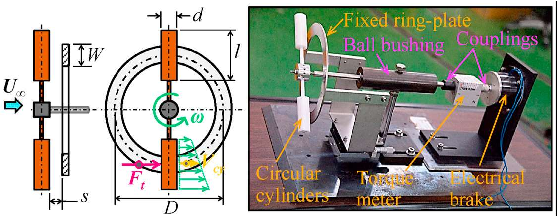
\includegraphics[width=0.8\textwidth]{figs/hemsuwanTurbine}
  \caption{Steady lift production from streamwise vortex. Adapted from \citet{Hemsuwan2021}.}
  \label{fig:hemsuwanTurbine}
\end{figure}

The two cylinders placed just upstream the ring plate, with the centre of the small rod coinciding with the centre of the ring plate. The result of the steady lift acting on the cylinders is the rotation of the rod with the two cylinders at its ends and the centre of the ring plate as its centre of rotation - creating essentially a turbine for fluid energy harvesting.

A lot of studies on this new type of energy harvester focuses on exploring the parameter space of variables that are hypothesised as having some significant degree of influence on the resulting torque or power. For example the study of \citet{Hemsuwan2021} explored the parameters ring plate width and exposed blade length, while \citet{Sakamoto2021} the gap between the circular cylinder blade and ring plate, and flange separation length. All these variables investigated exhibits optimum points that are typical in the study of turbine performance. Although this is a novel variation on the cruciform-type harvesters and seems very promising, the power output and efficiency is still far behind conventional wind turbines by several orders of magnitude.

Apart from these studies, the present work is not aware other attempts to generalise the cruciform oscillator system and further unlock the vortical structure and cylinder vibration-regulating potential of the strip plate, which might hold the key to further improving its power output and efficiency.

\section{Methodologies in VIV Studies} \label{sec:vivMethods}

\subsection{Vibration Parameters} \label{ssec:vibPara}

\begin{figure}[!h]
  \centering
  \hspace{1cm} 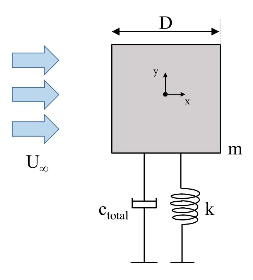
\includegraphics[width=0.35\textwidth]{figs/shafinazFBD}
  \caption{The free-body diagram of \citet{Maruai2019}.}
  \label{fig:shafinazFBD}
\end{figure}

Consider the free-body diagram (FBD) of \citet{Maruai2019}, shown in Fig. \ref{fig:shafinazFBD}. The vibrating cylinder, which in this case is a square cylinder, is modelled as being connected to a spring and damper with coefficients $k$ and $c_{\text{total}}$, respectively. For this study, since the thesis is dealing with a cruciform oscillator, the FBD is as shown in Fig. \ref{fig:freeBodyDiagram}. The FBD also consists of a cylinder, this time a circular cylinder, and a strip plate is placed is placed downstream at a gap of $G=0.16$.

\begin{figure}[!h]
  \centering
  \hspace{1cm} 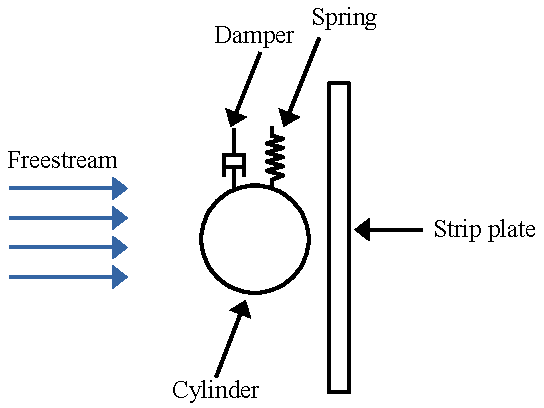
\includegraphics[width=0.6\textwidth]{figs/freeBodyDiagram}
  \caption{The free-body diagram of the cruciform oscillator.}
  \label{fig:freeBodyDiagram}
\end{figure}

For a vibration system with an effective mass $m_{\text{eff.}}$, spring coefficient $k$ and damping constant $c_{\text{tot.}}$, the total damping coefficient becomes

\begin{equation}
  \zeta_{\text{tot.}} = \frac{c_{\text{tot.}}}{2 \sqrt{k m_{\text{eff.}}}}.
  \label{eq:zetaTotal}
\end{equation}

\noindent The way damping is measured for a vibrating system is through free-vibration tests \citep{Sinha2010} in the medium the system is submerged in. For systems that vibrate in water, the free-vibration tests are also done in water. When a free-vibration test is done on the cylinder in Fig. \ref{fig:freeBodyDiagram}, the cylinder displacement time series $y=y(t)$ registers a reading as shown schematically in Fig. \ref{fig:freeVibration}.

\begin{figure}[!h]
  \centering
  \hspace{1cm} 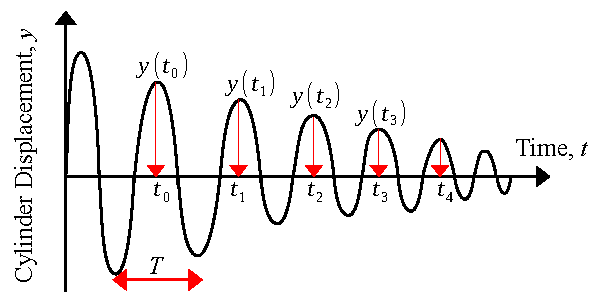
\includegraphics[width=0.7\textwidth]{figs/freeVibration}
  \caption{Free-vibration response of the vibrating system.}
  \label{fig:freeVibration}
\end{figure}

\noindent Here, $t_{0}, \, t_{1}, \, ... \, , \, t_{n}$ are the locations of the peaks in the free-vibration response. When the mean vibrating period $T$ is defined as

\begin{equation}
  T = \frac{t_{n} - t_{0}}{n},
  \label{eq:meanPeriod}
\end{equation}

\noindent a quantity called the logarithmic decrement $\delta$ can be defined such that

\begin{equation}
  \delta = \frac{1}{n} \text{ln} \left( \frac{y(t_{0})}{y(t_{n})} \right).
  \label{eq:logDecrement}
\end{equation}

\noindent In doing so, the damping coefficient can be computed \citep{Sinha2010} using the following relationship.

\begin{equation}
  \zeta_{\text{tot.}} = \frac{\delta}{\sqrt{4 \pi^{2} + \delta}}
  \label{eq:dampingCoeff}
\end{equation}

\noindent Literature on VIV-energy harvesters of the single cylinder kind, for example \citet{Yuan2020} and \citet{Kim2021}, generally specifies their value system damping using the damping coefficient $\zeta_{\text{tot.}}$. However, VIV-energy harvesters of the cruciform kind, for example \citet{Adzlan2021} and \citet{Mohamed2021}, usually specify their system damping using the Scruton number Sc,

\begin{equation}
  \text{Sc} = \frac{8 m_{\text{eff.}} \delta}{\rho \pi D^{2} l}.
  \label{eq:scrutonNo}
\end{equation}

\noindent Here, $l$ is the spanwise length of the cylinder. Knowing the value of $\delta$ also allows the computation of the system natural frequency $\fn$,

\begin{equation}
  \fn = \frac{\sqrt{4 \pi^{2} + \delta^{2}}}{2 \pi T}.
  \label{eq:naturalFrequency}
\end{equation}

\subsection{Solution of Governing Equations} \label{ssec:govEquations}

The numerical part of this study utilises OpenFOAM, an open-source computational fluid dynamics (CFD) platform written in C++. OpenFOAM solves the 3D unsteady Reynolds averaged Navier-Stokes (3D URANS) equations that are the following.

\begin{equation}
  \frac{\partial U_{i}}{\partial x_{i}}=0,
  \label{eq:continuity}
\end{equation}

\begin{equation}
  \frac{\partial U_{i}}{\partial t}+U_{j}\frac{\partial U_{i}}{\partial x_{j}} = -\frac{1}{p}\frac{P}{x_{i}}+\frac{\partial}{\partial x_{j}} \left( 2\nu S_{ij}-\overline{u'_{j}u'_{i}} \right).
  \label{eq:navier-stokes}
\end{equation}

\noindent The symbols $U$, $x$, $t$, $\rho$, $P$, $\nu$, $S$, and $u'$ denote the mean component of velocity, spatial component, time, density, pressure, kinematic viscosity, mean strain rate and the fluctuating component of velocity, respectively. Equation \ref{eq:sij} gives the mean strain rate $S_{ij}$.

\begin{equation}
  S_{ij} = \frac{1}{2} \left( \frac{\partial U_{i}}{\partial x_{j}} + \frac{\partial U_{j}}{\partial x_{i}} \right).
  \label{eq:sij}
\end{equation}

The turbulence model that approximates the Reynolds stress tensor is the Spalart-Allmaras turbulence model. Previous numerical studies on energy harvesting from FIM of circular cylinders have shown reasonable agreement with experiments in the literature through the use of this turbulence model, and thus becomes the basis for the implementation of the same turbulence model in this study \citep{Ding2015a,Ding2015b}. The Boussinesq approximation relates the Reynolds stress tensor $\tau_{ij} = \overline{u'_{j}u'_{i}}$ to the mean velocity gradient, exemplified by Eq. \ref{eq:tauij}.

\begin{equation}
  \tau_{ij} = 2 \nu_{T}S_{ij},
  \label{eq:tauij}
\end{equation}

\noindent where $\nu_{T}$ represents the kinetic eddy viscosity. This kinetic eddy viscosity is ultimately expressed as a function whose arguments consist of the molecular viscosity $\nu$, and an intermediate variable $\tilde{\nu}$ that is the solution of Eq. \ref{eq:kineticEddyTransport}. Equation \ref{eq:kineticEddyTransport} incorporates empirically obtained constants to provide closure to the equations governing this numerical investigation. The empirical constants that make up Eq. \ref{eq:kineticEddyTransport} are listed in Table \ref{tab:spalart-Allmaras}.

\begin{equation}
  \label{eq:kineticEddyTransport}
  \frac{\partial \tilde{\nu}}{\partial t} + U_{j} \frac{\partial \tilde{\nu}}{\partial x_{j}} = c_{b1}\tilde{S}\tilde{\nu} - c_{w1} f_{w} \left( \frac{\tilde{\nu}}{D} \right)^{2} + \frac{1}{\sigma} \left\{ \frac{\partial}{\partial x_{j}} \left[ \left( \nu + \tilde{\nu} \right) \frac{\partial \tilde{\nu}}{\partial x_{j}} \right] + c_{b2} \frac{\partial \tilde{\nu}}{\partial x_{i}} \frac{\partial \tilde{\nu}}{\partial x_{i}} \right\}
\end{equation}

\begin{table}[!ht]
\centering
\caption{Empirical constants used in the Spalart-Allmaras turbulence model.} \label{tab:spalart-Allmaras}
\vspace{\baselineskip}
\begin{tabular}{l c}
  \hline
  \hline

  Empirical constants & Value    \\
  \hline

  $c_{b1}$            & $0.01$   \\
  $c_{b2}$            & $0.09$   \\
  $c_{\nu1}$          & $0.01$   \\
  $\kappa$            & $0.1$    \\
  $\sigma$            & $0.162$  \\
  $c_{\omega3}$       & $0.178$  \\
  \hline
  \hline
\end{tabular}
\end{table}

\noindent The interested reader is referred to the original paper by \citet{Spalart1992} and more recent applications of the turbulence model in \citet{Ding2019} and \citet{Sun2019b}. With the turbulence model properly defined, one is finally able to solve Eqs. \ref{eq:continuity} and \ref{eq:navier-stokes} using the SIMPLE-stabilised PISO algorithm native to OpenFOAM, known as the PIMPLE algorithm.

\subsection{Dynamic Mesh Motion} \label{ssec:dynMesh}

Cylinder motion in the computational domain due to FIV introduces distortion to the mesh immediately surrounding the cylinder. The simplest way to keep the mesh distortion in check, thus keeping mesh quality within an acceptable level, is by diffusing the amount of warping to the surrounding space. In practice, the surrounding space is the rest of the mesh nodes, and Eq. \ref{eq:laplace} governs the diffusion.

\begin{equation}
  \nabla \cdot \left( \gamma \nabla u \right) = 0.
  \label{eq:laplace}
\end{equation}

\noindent Here, $\nabla$ is the differential operator equivalent to

\begin{equation}
  \nabla = \left( \frac{\partial}{\partial x}, \frac{\partial}{\partial y}, \frac{\partial}{\partial z} \right),
  \label{eq:nabla}
\end{equation}

\noindent in a three-dimensional Cartesian coordinate system.

In Eq. \ref{eq:laplace}, $u$ and $\gamma$ represents the mesh deformation velocity and displacement diffusion, respectively. In this work, the displacement is diffused according to the inverse quadratic rule $\gamma = 1/l^{2}$. Here, $l$ denotes the distance from the cell centre to the nearest cylinder edge. Diffusing the mesh deformation by the inverse quadratic rule means that a lot more deformation is diffused in the region closer to the surface of the cylinder compared to the region further away.

Then, Eq. \ref{eq:laplace} is solved using the generalised geometric-algebraic multi-grid (GAMG) algorithm and the Gauss-Seidel smoother. Solution of Eq. \ref{eq:laplace} returns an updated value of $u$, and this updated value of $u$ is used to update the position of the mesh nodes according to Eq. \ref{eq:meshNodeUpdate}. The PIMPLE solver resumes the solution of the 3D URANS equations after the mesh node positions are updated.

\begin{equation}
  x_{\text{new}} = x_{\text{old}} + u \Delta t
  \label{eq:meshNodeUpdate}
\end{equation}

\noindent Here, $u$ is the mesh deformation velocity, $\Delta t$ the time step for numerical solution, $x_{\text{old}}$ the previous mesh node position and $x_{\text{new}}$ the new mesh node position.

For most numerical studies of fluid-structure interaction (FSI), the mesh warp diffusion method governed by Eq. \ref{eq:laplace} serves as an adequate workaround to conserve mesh quality. However, this requires ample number of ambient mesh nodes acting as the receiving end of the diffusion algorithm. In this case, the small gap between the cylinder and strip plate ($G = 0.16$) pose a serious limitation to the ability to diffuse the amount of warp introduces by the displacement of the cylinder, since a small space means that one can only allocate a proportionate number of mesh nodes in said gap. Sole reliance on the warp diffusion algorithm will hamper the effort to preserve mesh quality as a high concentration of warp remains within the gap.

To overcome this problem, the arbitrarily coupled mesh interface (ACMI) is implemented halfway through the gap (see Figs. \ref{fig:probGeoSide}--\ref{fig:probGeoTop}). This technique allows adjacent cells to slide over each other precisely at the $x = 0.13$ plane, ridding this work of the requirement for mesh warp diffusion. In the literature, ACMI is also known as the generalised grid interface, or GGI in \citep{Zhang2018} and \citet{Sun2019b}. A more recent example of the implementation of ACMI can be found in \citet{Yang2022}, where ACMI is used to connect two differently meshed regions. This is shown in Fig. \ref{fig:acmi}.

The number of cells used in the spatial discretisation of the computational domains are determined from the grid independency study on the pure cruciform whose results are detailed in Chapter Four. Difference in the geometry of the cruciform model implemented in each study case results in a slightly different number of cells for each cruciform. However, all of them are ensured to exceed the minimum of 697608 cells, where the numerical results only differ only slightly with the expected value in the limit where the cell size approaches zero, hence number of cells approaching infinity. The $y^{+}$ values for each simulation is capped at $y^{+}< 15$, following \citet{Wang2019}. Here, $y^{+}$ is a measure of distance normal from the surface of the object submerged in the flow, taking into consideration the friction velocity $u^{*}$ \citep{Bhukta2018} and kinematic viscosity of the fluid such that

\begin{equation}
  y^{+} = \frac{u^{*} y}{\nu}.
  \label{eq:yplus}
\end{equation}

\noindent In this context, $y$ is simply the distance normal to the surface of the object submerged in the flow.

\begin{figure}[!h]
  \centering
  \hspace{1cm} 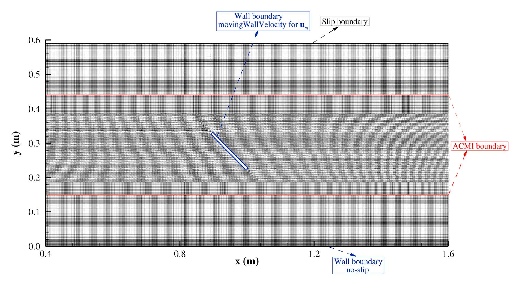
\includegraphics[width=0.95\textwidth]{figs/acmi}
  \caption{An example application of ACMI between two differently meshed regions. Adapted from \citet{Yang2022}.}
  \label{fig:acmi}
\end{figure}

The quality of the grid mesh is also established using the Richardson extrapolation and the grid convergence index (GCI) \citep{Stern2001}. The Richardson extrapolation \citep{Richardson1927} and GCI provides this study with a procedure to quantitatively measure on the degree of convergence for the quantities of interest in a numerical study. This method also forces the researcher to pay attention to the trend of convergence of the quantities of interest, requiring a monotonic convergence before proceeding to data collection, in line with previous research such as \citet{MatAli2011} and \citet{Maruai2018}. A good quality mesh is essential for the computation and visualisation of three-dimensional vortical structures using the $Q$-criterion. The $Q$-criterion is described in \citet{Jeong1995} as the region with positive second invariant of $\nabla U$ - the velocity gradient - where

\begin{equation}
  Q = \frac{1}{2} u_{i,j}u_{j,i}.
  \label{eq:qCriterion}
\end{equation}

\subsection{Ensemble Empirical Mode Decomposition and Hilbert Transform} \label{ssec:eemd}
%% Paraphrase in Grammarly BEGIN
The need to understand the time variation pattern of lift and cylinder displacement brings into the spotlight the ensemble empirical mode decomposition (EEMD) method \citep{Huang1998,Wu2008} as a signal processing tool, following which the computation of the instantaneous phase lag, frequency and amplitude are made possible using the Hilbert transform.

There is a strong precedent established in the literature on KVIV on the use of Hilbert transform (HT) to study the instantaneous phase and frequencies of the lift and displacement signals \citep{Khalak1999}. Regardless, the signal must fulfil several criteria for HT to realise its full potential. EEMD allows a larger class of signals to be meaningfully analysed using HT by decomposing the original signal into components that (1) have zero mean and (2) returns zero or one as the difference between the number of extrema and zero crossings. A physically meaningful HT result is assured for signals bound by these constraints. These signals are referred to in the literature as the intrinsic mode functions (IMF). Instead of fitting an a priori function of varying scales into the signal being processed - e.g. Fourier and wavelet transforms - EEMD is adaptive and is firmly grounded in the scales defined by the original signal.

Decomposing a signal using EEMD is procedural by design: produce 150 sets of white noise equal in length to the original signal. The amplitude of the white noise is set to one-fifths of the standard deviation of the original signal. Then, the original signal is superimposed on the set of white noises, thus creating 150 variations of the original signal. Next, the empirical mode decomposition (EMD) algorithm is run on the 150 constructed signals. The following describes the EMD algorithm.

\begin{enumerate} \label{enumerate:emd}
  \item Connect all extrema in the signal with third-order splines, creating an envelope. \label{enum:envelope}
  \item Trace the envelope mean for the whole data length. \label{enum:localMean}
  \item Compute the difference between the envelope mean and the original signal. \label{enum:difference}
  \item Iterate steps \ref{enum:envelope} and \ref{enum:localMean} on \ref{enum:difference} ten times \citep{Wu2008}.
\end{enumerate}

This algorithm produces intrinsic mode functions or IMFs for each of the 150 variations of the original signal. Then, the first IMF component is averaged from each of the 150 variations of the original signal to obtain the first EEMD IMF, $C_{1}$. The same is done for component number two, three, ..., $i$ for each of the 150 variations, producing $C_{2},C_{3},\dots,C_{i}$.

Since EEMD decomposes the original signal into $i$ number of IMFs, one needs to be selected among them to represent the original signal to compute phase lag. To achieve this, the original cylinder displacement signal is used as the reference. Then, the correlation between the IMFs from each decomposed $\cl$ and $\ystr$ signals are computed using cross-correlation. The IMF with the highest correlation coefficient is used in the phase lag computation, denoted as $\cysys$ for the cylinder displacement and $\cclys$ for the lift coefficient signal. Computation of the phase lag, instantaneous frequency and instantaneous amplitude of the signal is accomplished by constructing an analytical signal $z \left( t \right)$ from $C_{1},C_{2},\dots,C_{i}$ by computing the Hilbert transform of the IMF, $H_{i}$,

\begin{equation}
  H_{i} \left( t \right) = \frac{1}{\pi} \text{PV} \int\limits_{}^{\infty} \frac{C_{i} \left( \tau \right)}{t - \tau} d\tau,
  \label{eq:hilbertTransform}
\end{equation}

\noindent where PV denotes the Cauchy principal value, and then constructing the analytical signal as follows.
\begin{equation}
  z \left( t \right) = C_{i} \left( t \right) + i H_{i} \left( t \right) = a(t)e^{i\theta(t)},
  \label{eq:analiticalSignal}
\end{equation}

\noindent Note that $i$ in Eq. \ref{eq:analiticalSignal} is the complex number.
%% Paraphrase in Grammarly END
Also, $a(t)$ and $\theta(t)$ are the instantaneous amplitude and phase - both a function of time, and they are computed through the following equations.

\begin{equation}
  a(t) = \left( x^{2} + y^{2} \right)^{1/2},
  \label{eq:instAmplitude}
\end{equation}

\noindent and

\begin{equation}
  \theta(t) = \arctan{\frac{C_{i}}{H_{i}}}.
  \label{eq:instPhase}
\end{equation}

\noindent Computing the instantaneous frequency is therefore an exercise in differentiation, i.e.,

\begin{equation}
  \omega(t) = - \frac{d\theta}{dt},
  \label{eq:instFrequency}
\end{equation}

\noindent where $\omega(t)$ represents the instantaneous frequency of component $C_{i}$ of the original signal.


\section{Chapter Summary}
This chapter reviewed studies that contribute towards the advancement of vibration energy harvesting from alternating lift mechanisms, in particular the advancement of energy harvesting from cruciform systems. Figure \ref{fig:pyramidOfKnowledge} illustrates how the status quo of knowledge concerning energy harvesting from a cruciform is akin to the tip of the pyramid. Improving the performance of the cruciform energy harvester is heavily dependent on advances in other fields that are more fundamental, such as vortex-induced vibration and vortex shedding. Figure \ref{fig:pyramidOfKnowledge} also exemplifies the relative number of studies between the subjects, with the most number of studies over the years investigating the phenomenon of vortex shedding, especially Karman vortex shedding, followed by studies on the vibration responses of circular cylinder and cruciform oscillators, and finally, studies on energy harvesting using cruciform oscillators and the circular cylinder oscillator which they are based upon.

\begin{figure}[!h]
  \centering
    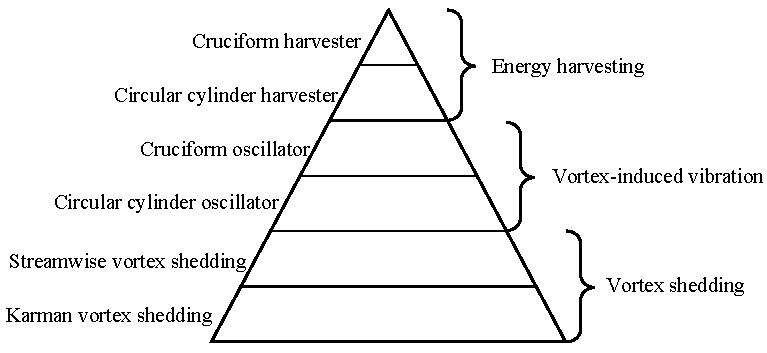
\includegraphics[width=\textwidth]{figs/pyramidOfKnowledge}
    \caption{The pyramid of knowledge for the cruciform energy harvester.}
    \label{fig:pyramidOfKnowledge}
\end{figure}

%%Chapter 2-9IE<<
The main takeaways from each literature reviewed in this chapter is summarised in Table \ref{tab:litRevSummary}. The state-of-the-art of Karman vortex shedding studies inform this thesis of the controllability of the vortex shedding through the modulation of the shear layer around the circular cylinder. Then, this work is informed that the three-dimensionality of Karman vortex brings about the formation of streamwise vortices of a scale smaller than the diameter of the circular cylinder, and whose dynamics are heavily influenced by the shedding of Karman vortices. Reviewing these literature updated our understanding on why and when streamwise vortices form in the first place. An improved understanding of this enables the proposal of new ideas on how to trigger the onset of SVIV at a lower Re or $\ured$. It can also help this thesis identify the causes of difference in amplitude and frequency response when KVIV changes to SVIV, which is objective one.

\begin{landscape}
  \thispagestyle{mylandscape}
  \begin{table}[p]
  \centering
  \caption{Summary of findings in literature and key takeaways.} \label{tab:litRevSummary}
  \vspace{\baselineskip}
  \begin{tabular}{p{4cm}>{\centering}p{2.5cm}>{\centering\arraybackslash}p{15cm}}
    \hline
    \hline

    Literature           & Type of study & Key takeaway \\
    \hline

    \citet{Asano2020} & Numerical & \multirow{5}{\hsize}{Karman vortex shedding can be controlled by modulating the shear layer of the circular cylinder. This is achieved through various methods, e.g., porous surface/outer layer and caviration bubbles.} \\
    \cline{1-2}
    \citet{Ledda2018}, \citet{Durhasan2019}, \citet{Geyer2020}, \citet{Kang2020}  & \multirow{5}{\hsize}{Experimental} & \\
    \hline
    \citet{Gibeau2018}, \citet{Gibeau2019}, \citet{Rai2018} & \multirow{3}{\hsize}{Experimental} & \multirow{3}{\hsize}{Small scale streamwise vortices originate from the three-dimensionality of Karman vortices, and the temporal dynamics of these streamwise vortices are dictated by the shedding dynamics of the Karman vortices.} \\
    \hline
    \citet{Lin2018}, \citet{Zhang2019}, \citet{Koide2017}  & \multirow{3}{\hsize}{Experimental} & \multirow{3}{\hsize}{Flow control due to placement of a downstream body is able to induce the shedding of large scale streamwise vortices, and the temporal dynamics of these streamwise vortices are independent of the shedding dynamics of coexisting Karman vortices.} \\
    \hline
    \citet{Ding2017}, \citet{Xu2017}, \citet{Yuan2020} & \multirow{3}{\hsize}{Experimental} & \multirow{3}{\hsize}{The amplitude/frequency response of a single cylinder oscillator unit can be modulated by tuning the mechanical parameters of the oscillator, e.g., adjusting the spacing between units, spring stiffness, system damping.} \\
    \hline
    \citet{Deng2007}   & Numerical & \multirow{4}{\hsize}{The amplitude/frequency response of a pure cruciform oscillator is heavily influenced by the spacing between the upstream and downstream cylinders. Optimising this parameter allows for very large range of synchronisation and a well-behaved upper limit to the vibration amplitude.} \\
    \cline{1-2}
    \citet{Kato2007}, \citet{Koide2013}, \citet{Zhao2018a}   & \multirow{3}{\hsize}{Experimental} &        \\
    \hline
    \citet{Ma2018}, \citet{Sun2019b} & \multirow{2}{\hsize}{Experimental} & \multirow{2}{\hsize}{In-tandem configuration of single cylinder harvester units are able to synergise and recover a large amount of power. The use of nonlinear springs can enhance this effect.} \\
    \hline
    \citet{Hemsuwan2018a,Hemsuwan2018b,Hemsuwan2018c}  & \multirow{2}{\hsize}{Numerical} &  \multirow{4}{\hsize}{Advances in cruciform energy harvesters are heavily focussed on recording the system responses due to cruciform parameter variation. Numerical studies are disrupting this trend.} \\
    \cline{1-2}
    \citet{Koide2009}, \citet{Nguyen2012} & \multirow{3}{\hsize}{Experimental} &  \\
    \hline
    \hline
\end{tabular}
  \end{table}
\end{landscape}

\noindent Then, the inclusion of a downstream cylinder such as another circular cylinder or a strip plate induces the shedding of streamwise vortices of a scale similar to the diameter of the upstream cylinder. These large-scale streamwise vortices are less under the influence of the Karman vortices compared to the small-scale streamwise vortices discussed previously. This highlights the need to understand what actually takes place in the flow field as the large-scale streamwise vortices form, which is what the first objective of this thesis tries to achieve, particularly why they modulate the lift signals as observed in the literature.

This chapter also highlights how the amplitude/frequency response of an oscillating system is influenced by varying mechanical parameters of the system and also geometry of the oscillator. This is especially pertinent in cruciform oscillators as the spacing between the upstream cylinder and downstream strip plate dictates the size of the synchronisation regime, which can be up to 15 times larger than the synchronisation regime of an elastically supported smooth circular cylinder. The fact that not much is known about why the geometrical configuration of the cruciform influences the system response of the oscillator is the motivation behind objective two of this thesis, where the present work tries to describe the lift signal as comprised from a finite number of constituents.

Finally, this chapter revealed how the future of alternating lift energy harvesting lies in teasing out favourable flow structures from a system that is made of more than one cylinder. In particular, the VIV-based cruciform system whose studies up until the present is heavily reliant on probes and simple dye visualisations. This can benefit from advances in CFD and a relatively improved access to computing facilities, to investigate and evaluate novel geometrical configurations of the cruciform oscillator for energy harvesting. Following this literature review, it is found that there has been no effort from the research community to investigate cruciform energy harvesters except when the cruciform is right-angled. In fulfilling objective three of this thesis, a new parameter will be studied in this thesis, which is the cruciform angle. Then, the performance of this type of cruciform energy harvester will be evaluated to fulfil objective three.
%%Chapter 2-9IE>>

The next chapter discussses the methods employed to achieve all three objectives.

\chapter{Methodology} \label{chap:method}

The methodology flowchart is presented in Fig. \ref{fig:flowChartA} and Fig. \ref{fig:flowChartB}.

\begin{figure}[!h]
  \centering
  \hspace{1cm} 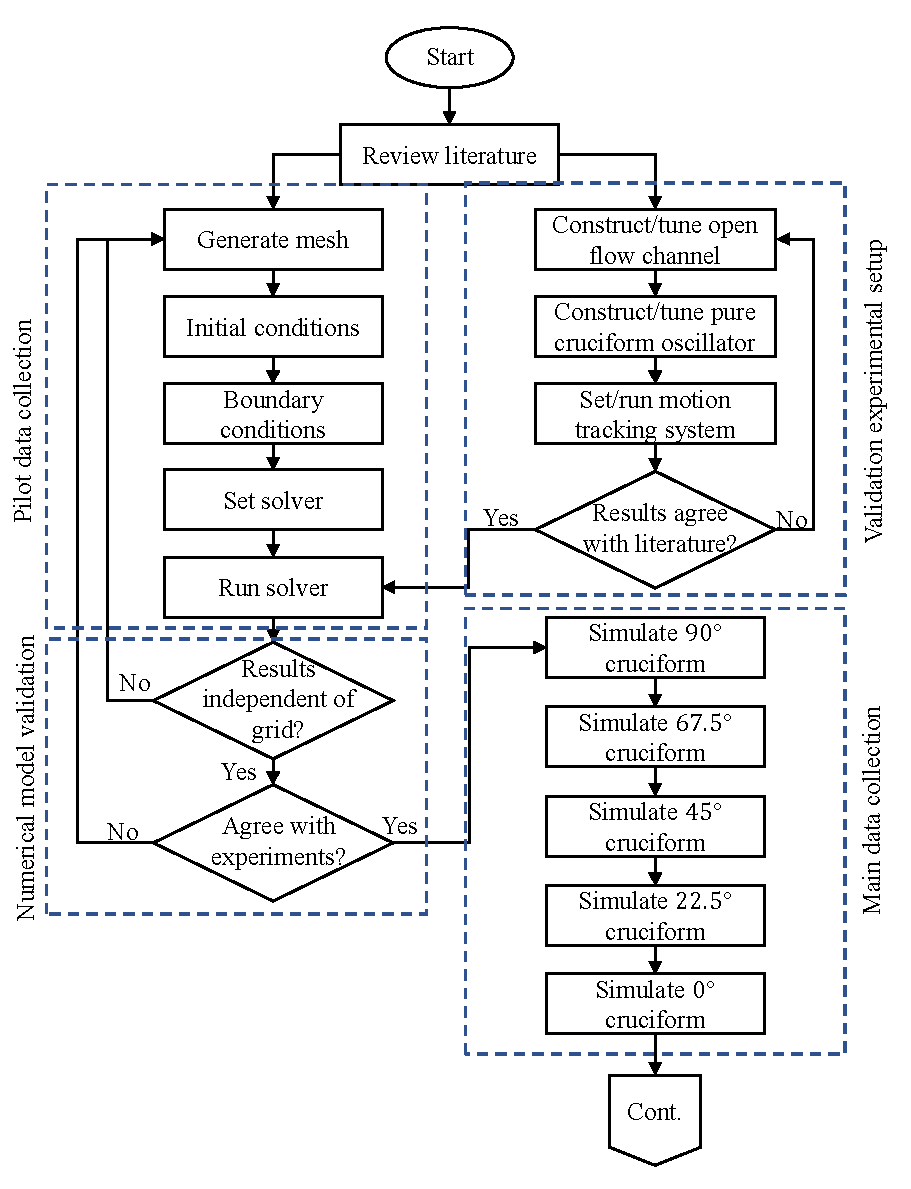
\includegraphics[width=0.9\textwidth]{figs/flowChartA}
  \caption{The first part of the methodology. This includes the pilot data collection, validation of numerical model and main data collection.}
  \label{fig:flowChartA}
\end{figure}

\begin{figure}[!h]
  \centering
  \hspace{1cm} 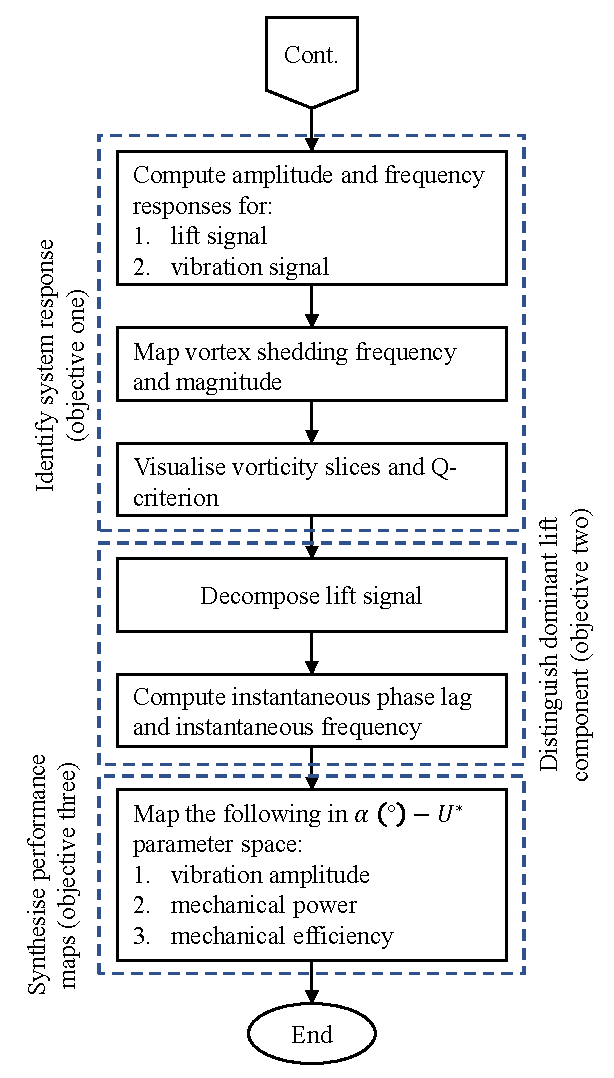
\includegraphics[width=0.7\textwidth]{figs/flowChartB}
  \caption{The second part of the methodology. This covers the data analysis part of the study.}
  \label{fig:flowChartB}
\end{figure}

\noindent After the literature review in Fig. \ref{fig:flowChartA}, the pilot data collection is initiated. This phase is where the study builds and refines the numerical model to be used for the rest of the data collection. Simulataneously, an experimental setup is constructed for the purpose of validating the results coming from the numerical data. The experiment only collects the vibration signal, i.e., cylinder displacement data for the pure cruciform case, between $1.1 \times 10^{3} \leq \re \leq 1.1 \times 10^{4}$. Then comes the grid convergence index study phase, to check the reliability of the numerical results. The numerical results are also checked against the validating experimental data.

 Next, the analysis phase in Fig. \ref{fig:flowChartB}. Analysis starts with computing the system response of the lift and vibration signals. This phase also includes the investigation of the causes that result in the system responses observed, to achieve objective one. After that comes the time series analysis phase of the lift signal. Here, the lift signal is analysed using HHT to distinguish the dominant component of lift, to answer objective two. Finally, the performance maps synthesis phase. This is the phase where the performance parameters of the cruciform energy harvester are mapped in the $\alpha \; (\si{\degree}) - \ured$ parameter space, to answer objective three.

 %%Chapter 3-2IE<<
\section{Design Geometry} \label{sec:probGeo}
%%Chapter 3-2IE>>

This study bases itself on the work done by \citet{Koide2013}, \citet{Maruai2017}, and \citet{Maruai2018}. In these works, the investigators conducted both experimental and computational investigations of passive control of fluid-structure interaction (FSI) of cylinders using a strip plate located at the cylinder downstream. Here, the term ``strip plate'' is used as a shorthand for the long, rectangular plate used to control the vibration of the cylinder -- since the plate resembles a strip due to its large aspect ratio. \citet{Koide2013} and \citet{Maruai2018} demonstrated the feasibility of energy harvesting using the oscillator system described.

% In the Reynolds number range $3.6 \times10^{3} < \text{Re} < 1.3 \times10^{4}$. Hence, a similar Re range for this thesis is chose. However, this study starts at $\re = 1.1 \times 10^{3}$ instead of $3.6 \times 10^{3}$, and stops at $\re = 1.5 \times 10^{4}$ instead of $1.3 \times 10^{4}$. This is done to allow examination of a slightly wider range of Re, compared to the previous studies of \citet{Koide2013}, \citet{Maruai2017}, and \citet{Maruai2018}.

%%Chapter 3-3IE<<
The oscillator system in this work derives its geometry from the works of \citet{Nguyen2012}, \citet{Koide2013}, and \citet{Koide2017}. The basic layout of the oscillator system is the pure cruciform: an arrangement where the circular cylinder and the strip plate located downstream have their axes perpendicular to each other. The gap between the cylinder and the strip plate, $G$, is fixed to $0.16$. This value of $G$ was chosen because the cylinder response most suitable for energy harvesting is sustained over the largest range of reduced velocity $\ured$ when $G = 0.16$ \citep{Koide2013}. The main parameters that set the scope of this study are the Reynolds number Re, reduced velocity $\ured$, Scruton number Sc and system natural frequency $\fn$ (Hz). The values of these parameters in previous studies are summarised in Table \ref{tab:parameterRange}.

\begin{table}[!ht]
\centering
\caption{Values of parameters investigated in previous studies.} \label{tab:parameterRange}
\vspace{\baselineskip}
\setlength{\tabcolsep}{10pt}      % This is the table column padding. Default value: 6pt
\renewcommand{\arraystretch}{1.5} % This is the table row padding. Default value: 1
\begin{tabular}{l c l}
  \hline
  \hline
Parameter                & Value                                         & Paper              \\ \hline
\multirow{3}{*}{Re}      & $1.1 \times 10^{3} < \re < 4.4 \times 10^{4}$ & \citet{Koide2013}  \\
                         & $1.4 \times 10^{3} < \re < 5.7 \times 10^{3}$ & \citet{Koide2017}  \\
                         & $4.2 \times 10^{3} < \re < 1.1 \times 10^{4}$ & \citet{Maruai2018} \\
                         & $3.6 \times 10^{3} < \re < 1.3 \times 10^{4}$ & \citet{Maruai2019} \\ \hline
\multirow{3}{*}{$\fn$}   & $4.5 < \fn \; (\text{Hz}) < 5.13$             & \citet{Nguyen2012} \\
                         & 4.4 Hz                                        & \citet{Koide2013}  \\
                         & 14.3 Hz                                       & \citet{Maruai2018} \\
                         & 14.3 Hz                                       & \citet{Maruai2019} \\ \hline
\multirow{3}{*}{$\ured$} & $2.2 < \ured < 88.7$                          & \citet{Koide2013}  \\
                         & 6, 8.5, 18                                    & \citet{Maruai2018} \\
                         & $4 < \ured < 20$                              & \citet{Maruai2019} \\ \hline
\multirow{3}{*}{Sc}      & 2.2                                           & \citet{Nguyen2012} \\
                         & 7.74                                          & \citet{Koide2013}  \\
                         & 31.12                                         & \citet{Maruai2019} \\
  \hline
  \hline
\end{tabular}
\end{table}

The primary constraint to the scope of this study is the range of Re. As summarised in Table \ref{tab:parameterRange}, it is apparent that the studies have their Re range starting at the end of TrSL1 and ends before the end of TrSL2. The exact value of the range is however, constrained by the choice of cylinder diameter and the freestream velocity that one is able to recreate in the laboratory or computer simulation. This thesis chose a diameter of 10 mm due to the physical dimension of the open flow channel for conducting the validating experiment. The open flow channel is able to produce $0.1 \leq U \; (\si[per-mode=symbol]{\metre\per\second}) < 1.1$. The computing facilities available to the author allow the simulation of up to 1.3 m/s of freestream velocity while keeping the total simulation time below three weeks, or twenty-one days. Therefore, the Re range for this study becomes $1.1 \times 10^{3} \leq \re \leq 1.5 \times 10^{4}$. This range also starts at the end of TrSL1 and ends before the end of TrSL2 - consistent with the studies referenced in Table \ref{tab:parameterRange}.

Once the Re range is set, the range of $\ured$ is determined exclusively by the system natural frequency $\fn$ (Hz). In the studies referenced in Table \ref{tab:parameterRange}, those working in a water flow have their $\fn$ set between 4.4 Hz to 5.13 Hz, while those working in an air flow have their $\fn$ set to 14.3 Hz. This thesis chose a value of $\fn = 4.42$ Hz as this study is conducted in a water flow. Consequently, the range for $\ured$ becomes $2.2 \leq \ured \leq 29.5$.

Finally, the values of Sc in Table \ref{tab:parameterRange} are 2.2 \citep{Nguyen2012} and 7.74 \citep{Koide2013} in a water medium, and 31.12 in an air medium \citep{Maruai2019}. The value of Sc for this study is 9.94, which is the result of having a larger effective mass $m_{e}$ compared to \citet{Nguyen2012} and \citet{Koide2013}.
%%Chapter 3-3IE>>

\begin{figure}[!h]
  \centering
  \hspace{1cm} 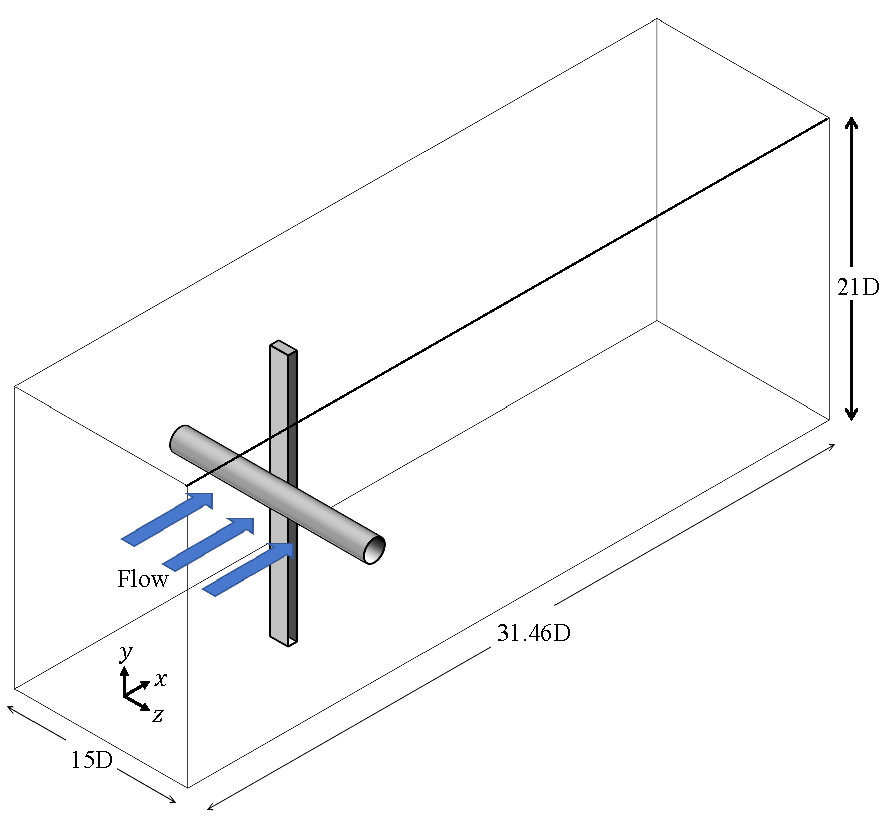
\includegraphics[width=0.8\textwidth]{figs/threeDimensionalDomain}
  \caption{Schematic of the computational domain.}
  \label{fig:threeDimDom}
\end{figure}

Figure \ref{fig:threeDimDom} shows the isometric view of the computational domain. The computational domain has a spanwise ($z$-direction) length of $15D$, a streamwise ($x$-direction) length of $31.46D$, and a height ($y$-direction length) of $21D$. The freestream flows from left to right. The strip plate has a thickness of $D/3$.
% Figure \ref{fig:probGeoSide} visualises the computational domain (Fig. \ref{fig:threeDimDom}) from its side. The streamwise coordinates of this domain extends from $-10.5D$ to $10.5D$, and the lateral coordinates from $-10.5D$ to $10.5D$. The coordinate origin $(0,0,0)$, is at the centre of the cylinder and the strip plate is $D/3$ thick.

\begin{figure}[!h]
  \centering
  \hspace{1cm} 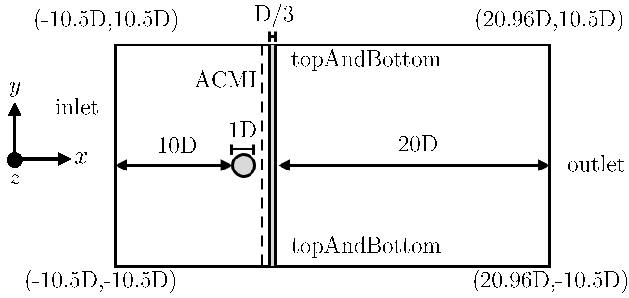
\includegraphics[width=0.9\textwidth]{figs/problemGeometrySide}
  \caption{The three-dimensional domain, side view.}
  \label{fig:probGeoSide}
\end{figure}

The coordinate system used in the domain has its origin (0,0,0) at the centre of the circular cylinder. Figure \ref{fig:probGeoSide} illustrates how this is the case, by presenting the side view of the computational domain, i.e., viewed from the positive $z$-direction. As shown in Fig. \ref{fig:probGeoSide}, the inlet plane has an $x$-coordinate of $-10.5D$. As the leading edge of the cylinder is $10D$ away from the inlet plane, and the cylinder has a diameter of $1D$, the origin of the $x$-axis is at the centre of the circle. Furthermore, the top plane and bottom plane of the domain is assigned $y$-coordinates $10.5D$ and $-10.5D$, respectively. Consequently, the origin of the $y$-axis is also at the centre of the circle.

\begin{figure}[!h]
  \centering
  \hspace{1cm} 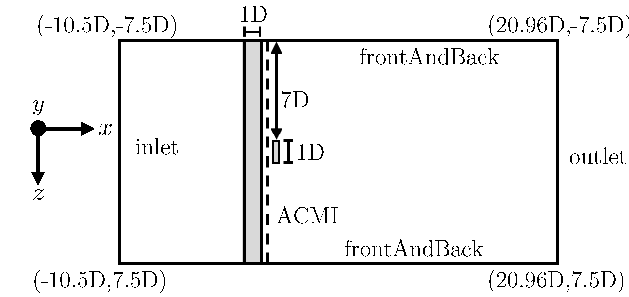
\includegraphics[width=0.9\textwidth]{figs/problemGeometryTop}
  \caption{The three-dimensional domain, top view.}
  \label{fig:probGeoTop}
\end{figure}

The top view in Fig. \ref{fig:probGeoTop} shows that the front and back planes of the computational domain is assigned $z$-coordinates $7.5D$ and $-7.5D$, respectively. As a result, the origin of the $z$-axis is located at the midpoint of the circular cylinder.

Then, variants of the pure cruciform configuration are constructed by rotating the strip plate from \angfi{} to \angon{} in \angtw{} increments. In total, five different cruciforms are constructed, as shown in Figs. \ref{fig:cruciform90}--\ref{fig:cruciform00}. This selection of cruciform angles is to allow exploration of the $\alpha \; (\si{\degree})$--$\ured$ parameter space with the least amount of cruciform variation. This is due to the constraint imposed by the computational time needed to simulate each of the conditions studied in this thesis, which is detailed in Section \ref{sec:numericalSolution}. The dimensions of the computational domain remain fixed for all cruciforms, including the gap between the cylinder and the strip plate.

\begin{figure}[!h]
  \centering
  \hspace{1cm} 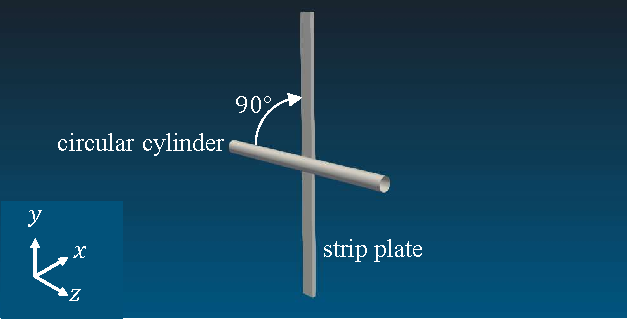
\includegraphics[width=0.7\textwidth]{figs/cruciform90}
  \caption{Cruciform layout for \angfi{}.}
  \label{fig:cruciform90}
\end{figure}

\begin{figure}[!h]
  \centering
  \hspace{1cm} 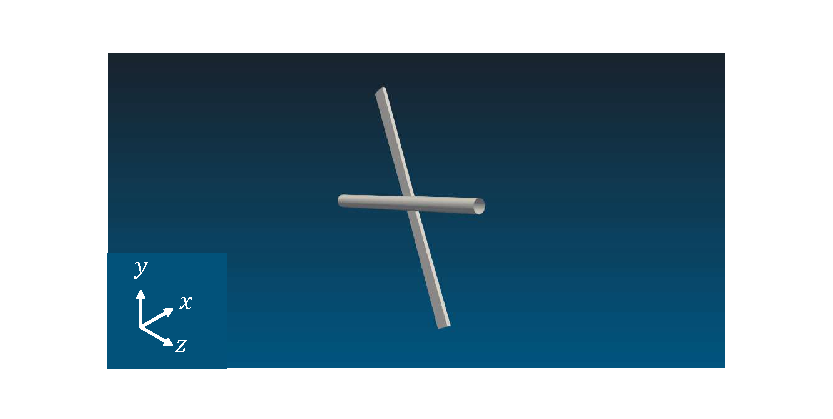
\includegraphics[width=0.7\textwidth]{figs/cruciform675}
  \caption{Cruciform layout for \angfo{}.}
  \label{fig:cruciform675}
\end{figure}

\begin{figure}[!h]
  \centering
  \hspace{1cm} 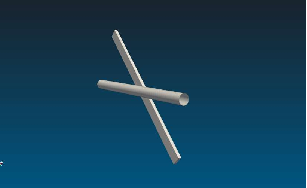
\includegraphics[width=0.7\textwidth]{figs/cruciform45}
  \caption{Cruciform layout for \angth{}.}
  \label{fig:cruciform45}
\end{figure}

\begin{figure}[!h]
  \centering
  \hspace{1cm} 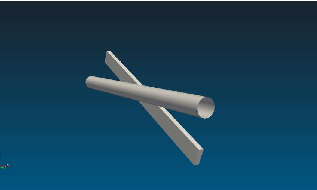
\includegraphics[width=0.7\textwidth]{figs/cruciform225}
  \caption{Cruciform layout for \angtw{}.}
  \label{fig:cruciform225}
\end{figure}

\begin{figure}[!h]
  \centering
  \hspace{1cm} 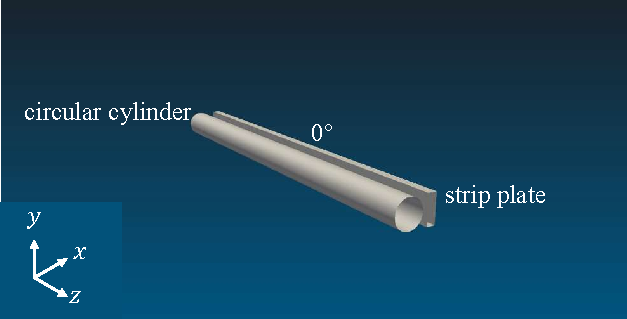
\includegraphics[width=0.7\textwidth]{figs/cruciform00}
  \caption{Cruciform layout for \angon{}.}
  \label{fig:cruciform00}
\end{figure}

To vary the angle of the cruciform, the cylinder is kept in its original location and maintains its orientation parallel to the $Z=0$ axis, while the strip plate is rotated in the counterclockwise direction when viewed from upstream. These cruciforms are studied within thirteen reduced velocities between $\uron \leq \ured \leq \urtt$, corresponding to $U = 0.1, 0.2, \cdots, 1.3$ m/s in freestream velocity.

\section{Numerical Solution} \label{sec:numericalSolution}

Table \ref{tab:researchMatrix} gives a summary of all conditions computed in the numerical study of this thesis. As this study seeks to understand the system response of a generalised form of cruciform oscillator, the angle between the cylinder and the strip plate is varied from the pure cruciform case (\SI{90}{\degree}) down to \SI{0}{\degree}, in \SI{22.5}{\degree} increments, as shown in Figs. \ref{fig:cruciform90}--\ref{fig:cruciform00}.

\begin{table}[!ht]
\centering
\caption{The list of conditions investigated in this study.} \label{tab:researchMatrix}
\vspace{\baselineskip}
\setlength{\tabcolsep}{10pt}      % This is the table column padding. Default value: 6pt
\renewcommand{\arraystretch}{1.5} % This is the table row padding. Default value: 1
\begin{tabular}{l c}
  \hline
  \hline
  Parameter                                  & Value or Range                                                     \\
  \hline
  Freestream velocity, $U$ (m/s)             & $0.1 \leq U \; (\si[per-mode=symbol]{\metre\per\second}) \leq 1.3$ \\
  Reduced velocity, $\ured$                  & $2.3 \leq \ured 29.5$                                              \\
  Reynolds number, Re                        & $1.1 \times 10^{3} \leq \re \leq 1.5 \times 10^{4}$                \\
  Cruciform angle $\alpha \; (\si{\degree})$ & $0 \leq \alpha \; (\si{\degree}) \leq 90$                          \\
  Cylinder diameter, $D$ (mm)                 & 10                                                                 \\
  Cylinder length, $l_{\text{cylinder}}$ (mm) & 10                                                                 \\
  Strip plate width (mm)                     & 10                                                                 \\
  Effective mass, $m_{\text{eff.}}$ (kg)     & 0.162                                                              \\
  Scruton number, Sc                         & 9.94                                                               \\
  System natural frequency, $\fn$ (Hz)       & 4.42                                                               \\
  \hline
  \hline
\end{tabular}
\end{table}

The numerical model designed in Figs. \ref{fig:threeDimDom}--\ref{fig:probGeoTop} is then solved using OpenFOAM. OpenFOAM discretises the continuity and three-dimensional unsteady Reynolds-averaged Navier-Stokes (3D URANS) equation and solves them over the specified mesh grid in the computational domain. The Spalart-Allmaras turbulence model is used to model the near-wall region of the simulation. The ACMI method is used to preserve mesh quality throughout the computational domain. Finally, identification of three-dimensional vortical structures are done using the $Q$-criterion, which can be computed automatically by OpenFOAM.

An HP Z420 workstation was used to perform the computations, and the specifications of the workstation are listed in Table \ref{tab:workstationSpec}. Since parallelisation is built into OpenFOAM, computationally exhaustive simulations can benefit a lot from being run on such a workstation with minimal effort from the end user. One can just specify the number of subdomains desired in each of the $x$, $y$, and $z$-directions, and then allocate one for each processor available in the workstation.

\begin{table}[!ht]
\centering
\caption{The specifications of the HP Z420 workstation} \label{tab:workstationSpec}
\vspace{\baselineskip}
\begin{tabular}{l l}
  \hline
  \hline

  Feature               & Description                            \\
  \hline

  Memory                & 38 GB                                  \\
  Processor             & Intel Xeon(R) CPU E5-16200 at 3.60 GHz \\
  Number of processors  & 16                                     \\
  Graphics              & Gallium 0.4 on NVE7                    \\
  Disk                  & 980.2 GB                               \\
  \hline
  \hline
\end{tabular}
\end{table}

However, due to the fact that the type of phenomena simulated in this study is three-dimensional, transient, turbulent and involves fluid-structure interactions, the simulations take a long time, even with the computational power listed in Table \ref{tab:workstationSpec}. To give the reader a perspective on this time length, consider the following example from one computational case. To simulate 20 s of flow time for the pure cruciform at $\ured = \urel$ ($U = 1.0$ m/s) using all 16 processors, the workstation took \SI{1688688}{\second} or approximately 19.5 days. This will only increase at higher freestream velocities as smaller time steps are required to maintain a Courant-Friedrichs-Lewy (CFL) number less than 1.

\section{Open flow channel experiment} \label{sec:openFlowExp}

As part of the validation process for the numerical setup, a closed loop open flow channel was constructed, with a test chapter \SI{100}{\milli\metre} wide, \SI{200}{\milli\metre} high and \SI{1500}{\milli\metre} long. The design of this open flow channel is heavily inspired by the water tunnel of \citet{Nguyen2012} and \citet{Koide2013}. Considering the application of this research in the far future is in open flows such as natural drainage systems or the ocean - and not within pipes - prompts this study to make this distinction.

\begin{figure}[!h]
  \centering
  \hspace{1cm} 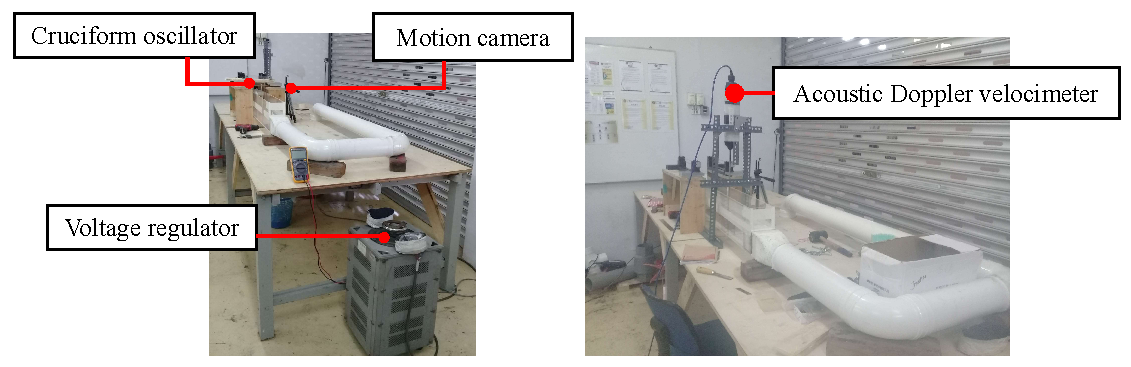
\includegraphics[width=0.95\textwidth]{figs/actualApparatus}
  \caption{The experimental apparatus used to validate the pilot numerical results.}
  \label{fig:actual apparatus}
\end{figure}

The open flow channel in Fig. \ref{fig:actual apparatus} is benchmarked by setting up a pure cruciform oscillator (\angfi{}) experiment, whose data from similar studies are readily available in published works. Following this, the rig is dimensioned to follow the parameters used in \citet{Koide2013}. A summary of the parameters and those used in \citet{Koide2013} are provided in Table \ref{tab:expParameter}. The parameters governing the amplitude/frequency response of the oscillator is tuned using simple length-based mechanism as follows (see Fig. \ref{fig:rigSketch}). To tune the spring coefficient $k$, one simply adjust the active length of the twin spring plate. In practice, the calibration curve of the twin spring plate is obtained by performing a weight - displacement measurement \citep{Sun2016} at several active lengths of the plate. Once the spring coefficient versus spring plate active length calibration curve is obtained, one can just adjust the length of the spring plate to achieve the desired value of $k$.

\begin{table}[!ht]
\centering
\caption{Summary of experimental parameters in contrast to those used in the experimental work of \citet{Koide2013}.} \label{tab:expParameter}
\vspace{\baselineskip}
\begin{tabular}{l c c}
  \hline
  \hline
                                           & Current study & \citet{Koide2013}\\
  \hline
Cylinder diameter, $D$ (m)                 & $0.01$        & $0.01$           \\
Cylinder length, $l_{\text{cylinder}}$ (m) & $0.09$        & $0.098$          \\
Strip-plate width (m)                      & $0.01$        & $0.01$           \\
Strip-plate length (m)                     & $0.1$         & $0.1$            \\
Effective mass, $m_{\text{eff.}}$ (kg)     & $0.162$       & $0.174$          \\
Logarithmic damping, $\delta$              & $0.178$       & $0.24$           \\
Scruton number, Sc                         & $9.94$        & $7.74$           \\
System natural frequency, $f_{n}$ (Hz)     & $4.42$        & $4.4$ to $4.79$  \\
  \hline
  \hline
\end{tabular}
\end{table}

\begin{figure}[!h]
  \centering
  \begin{subfigure}[h]{0.75\textwidth}
    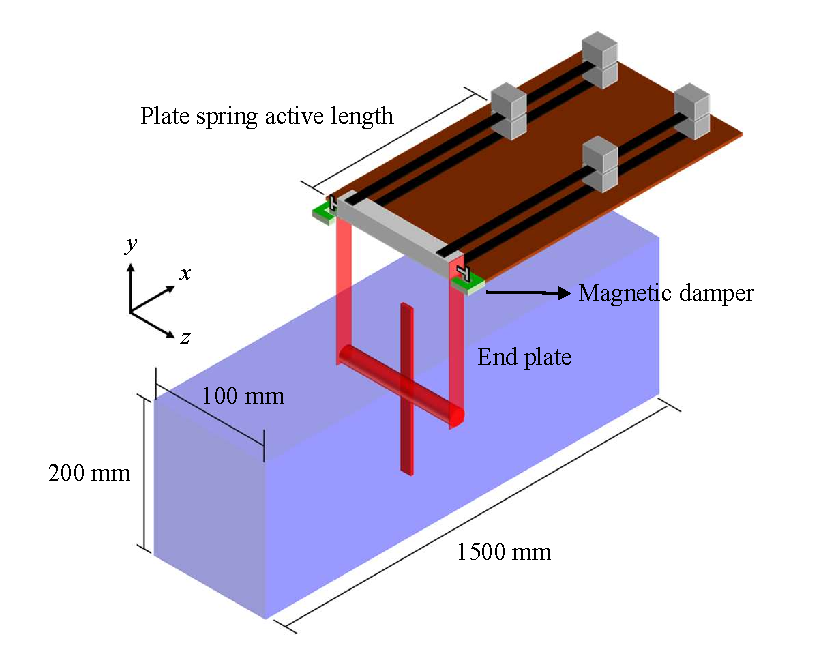
\includegraphics[width=\textwidth]{figs/rigSketch}
    \caption{Isometric sketch of the experimental setup.}
    \label{fig:rigSketch}
  \end{subfigure}

  \begin{subfigure}[h]{0.75\textwidth}
    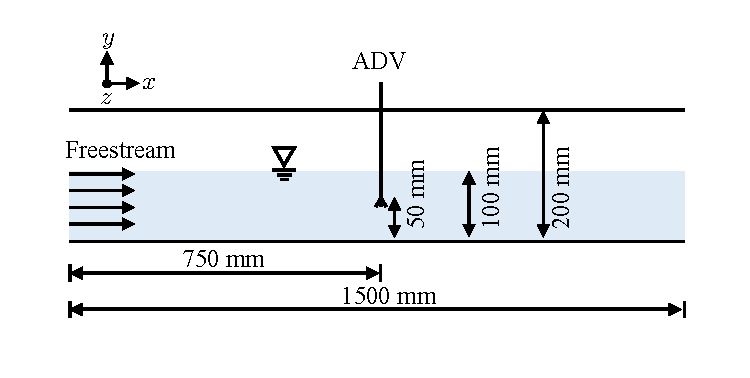
\includegraphics[width=\textwidth]{figs/channelSchematic}
    \caption{Side view of the openflow channel.}
    \label{fig:channelSchematic}
  \end{subfigure}

  \caption{Sketch of the experimental system used in this study.} \label{fig:experimentalSetup}
\end{figure}

Tuning the total damping of the system and consequently the multiple expressions of damping such as the logarithmic damping $\delta$, Scruton number Sc, or the damping coefficient is done by attaching, as shown in Fig. \ref{fig:rigSketch}, a T-shaped plate made from aluminium into a claw-shaped casing that houses neodymium magnets at its ends.

A voltage controller regulates the power driving the $3.728$ kW (5 hp) centrifugal pump. To set the freestream velocity in the open flow channel, an acoustic Doppler velocimeter (ADV) sampler is placed in an empty test chamber, filled with plain tap water to a height of \SI{100}{\milli\metre}, on the centreline of the channel, as pictured in Fig. \ref{fig:channelSchematic}. The height of \SI{100}{\milli\metre} is also the water level the experiments are in. The water level at \SI{100}{\milli\metre} is to achieve a flow ambience analogous to the benchmark study of \citet{Koide2013}.

The cylinder displacement $y$ is measured as a function of time by placing a visual marker on the support plate of the cylinder (see Fig. \ref{fig:rigSketch}) and capturing the motion of the marker using a video camera positioned perpendicular to the support plate. The motion of the marker is then analysed using \textit{Tracker}: a motion analysis tool built on the Open Source Physics Java framework (for recent implementation examples, see \citet{Wen2020}  or \citet{Krishnendu2020}).

\begin{figure}[!h]
  \centering
  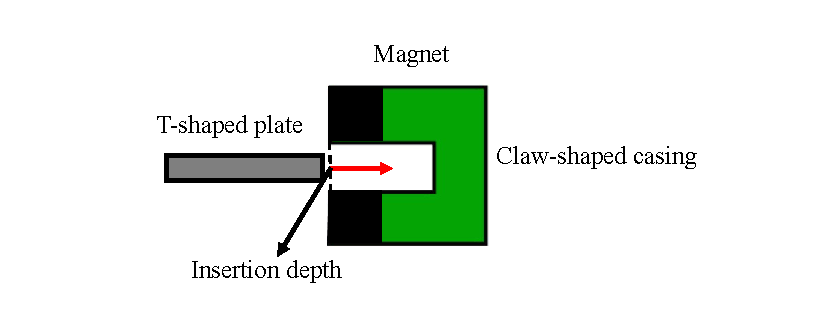
\includegraphics[width=1\textwidth]{figs/damperSketch}
  \caption{Close-up of the magnetic damper.}
  \label{fig:damperSketch}
\end{figure}

Figure \ref{fig:damperSketch} shows a close-up of the magnetic damper mechanism that provides damping for the apparatus in Fig. \ref{fig:rigSketch}. This method controls the strength of the magnetic field exposed to the T-shaped plate by fixing the insertion depth of the T-shaped plate into the casing. The magnetic field serves to dissipate the kinetic energy of the T-shaped plate that moves with the cylinder during VIV, providing system damping.

For the benchmarking, the reduced velocity $\ured = \urte$ is chosen. This is because the cylinder at that $\ured$ produces a large and stable displacement \citep{Koide2013}. A large and stable displacement simplifies the observation process. It also aids the comparison process between the experimental system and previous experimental studies, for example \citet{Koide2013}. The result of this benchmarking is presented in Section \ref{sec:appBenchmark}.

\section{Phase lag between $\cl$ and normalised cylinder displacement} \label{sec:phaseLag90}

In this study, the phase lag $\plag$ is computed by taking the Hilbert transform of both $\ystr$ and $\cl$ signals, as \citet{Khalak1999} did in their VIV study of isolated circular cylinders, finding the difference between them, and finally averaging the values over a selected period $T$. This is captured by Eq. \ref{eq:phaseLagDefinition}. The reason this quantity is computed is because there is a need to assign a representative value to the phase lag at each $\ured$, and the ensemble average is a deemed a reasonable statistical quantity that captures the essence of the temporal evolution of phase lag. Of course, differentiating the instantaneous phase with respect to time returns the instantaneous frequency.

\begin{equation}
  \plag = \frac{1}{T} \int_{0}^{T} \left[ \theta_{\text{Cl}}(t) - \theta_{y}(t) \right] dt.
  \label{eq:phaseLagDefinition}
\end{equation}

Out of $C_{i}$ IMFs for each of $\ystr$ and Cl, the ones for computation of instantaneous phase are selected according to the following rule. First, the IMF component of $\yrms$ with the largest \rms{} amplitude is selected to represent the original $\ystr$ signal. Then, the component of $\cl$ with the highest correlation to the IMF component of $\ystr$ is chosen, to represent the $\cl$ signal. The degree of correlation is determined by computing the cross-correlation between the two.

\section{Estimation of Power} \label{sec:estimationOfPower}

The mathematical model for harnessable power estimation in this study follows that which had been derived in \citet{Raghavan2007a}. Work done by the oscillating cylinder $\wcl$ during one cycle of oscillation $\tosc$ is

\begin{equation}
  \wcl = \int_{0}^{\tosc} \left ( \fl \cdot \dot{y} \right ) dt,
  \label{eq:workCylinder}
\end{equation}

\noindent where both the lift $\fl$ and cylinder velocity $\dot{y}$ are both functions of time. The fluid power is thus computed as

\begin{equation}
  \pfrms = \frac{1}{2} \rho \pi \cclrms U^{2} \fcyl \yrms D L \sin(\plag),
  \label{eq:rmsFluidPower}
\end{equation}

\noindent where $\fcyl$ is the vibration frequency of the cylinder. The mechanical power, on the other hand, is computed as

\begin{equation}
  \pmrms = 8 \pi^{3} \meff \zetatot \left (\yrms \fcyl \right )^{2} \fn.
  \label{eq:rmsMechPower}
\end{equation}

Here, $\pfrms$, $\pmrms$, $L$, $\cclrms$, $\zetatot$ and $\meff$ are the \rms{} of fluid power, \rms{} of mechanical power, length of the circular cylinder, characteristic \rms{} of lift amplitude, total damping coefficient, and the system effective mass respectively. The quantity $\cclys$ is used to represent $\cclrms$ in Eq. \ref{eq:rmsFluidPower}.

% The root-mean-square, i.e. \rms{} (parameters with subscript RMS) quantities in Eq. \ref{eq:workCylinder} instead of the maximum values like the original authors because that may lead to a misunderstanding that the maximum value is sustained throughout the observation window. This obviously is not always the case in this study, especially once the system transits into the SVIV regime. Recall that the time series analysis of $\ystr\left( t \right)$ and $\text{Cl}\left( t \right)$ in Chapter \ref{sec:svivRegime} revealed that there is a degree of intermittency in both signals that cannot be overlooked at certain ranges of $\ured$. Using the \rms{} value allows this work to partially take this into account in the estimation of harnessable power.

\section{Grid Independency Study} \label{sec:gridIndStu}

The pure cruciform configuration (the \angfi{} cruciform) is chosen as the benchmark case for grid independency study through the grid convergence index (GCI). This is because the vibration response for the pure cruciform is already available in the literature, and is also and collected as part of the validation step in this study. Data is collected at $\ured = \urte$ on three sets of grid numbered $1$ for the finest, $2$ for the medium and $3$ for the coarsest. A close-up of the grid 1 (fine), grid 2 (medium) and grid 3 (coarse) is shown in Fig. \ref{fig:threeGrids}. In this work, a refinement ratio of 1.376 is used from coarse to medium mesh, and a refinement ratio of 1.303 is used from medium to fine mesh. Computing the refinement ratio is done through the following method.

\begin{equation}
  r_{i+1,i} = \frac{S_{\text{grid},i+1}}{S_{\text{grid},i}},
  \label{eq:refinementRatio}
\end{equation}

\noindent where $S_{\text{grid},i}$ denotes the total number of cells in the $i^{\text{th}}$ grid.

Once the numerical solution has been shown to converge, the fine grid is used in all simulations of the pure cruciform case, and a similar mesh resolution is implemented on all cruciform variants studied in this work.

\begin{figure}[!h]
  \centering
  \begin{subfigure}[h]{0.3\textwidth}
    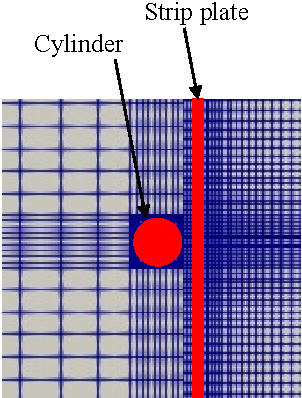
\includegraphics[width=\textwidth]{figs/threeGridsCoarse}
    % 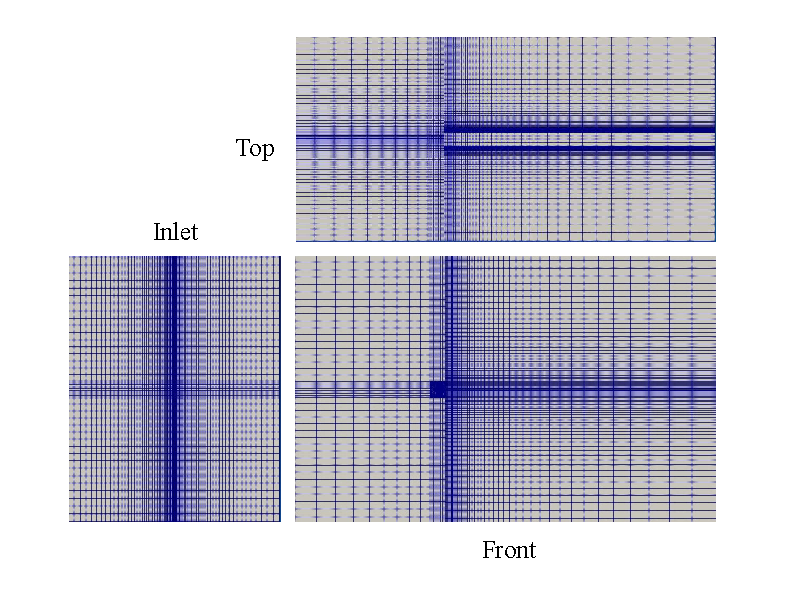
\includegraphics[width=\textwidth]{figs/figure6a}
    \caption{Coarse}
    \label{fig:coarseMesh}
  \end{subfigure} \hspace{0.25cm}
  \begin{subfigure}[h]{0.3\textwidth}
    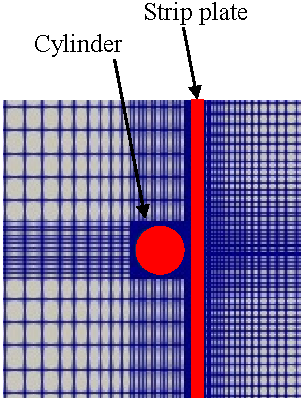
\includegraphics[width=\textwidth]{figs/threeGridsMedium}
    % 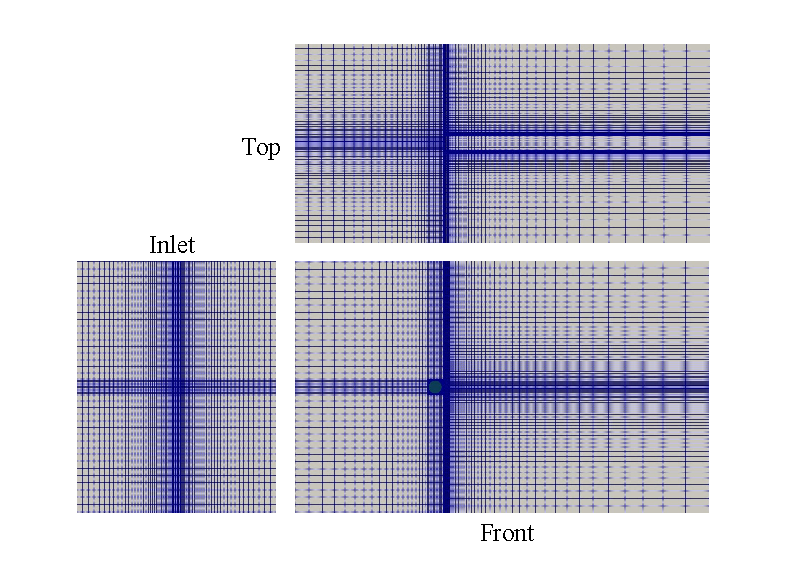
\includegraphics[width=\textwidth]{figs/figure6b}
    \caption{Medium}
    \label{fig:mediumMesh}
  \end{subfigure} \hspace{0.25cm}
  \begin{subfigure}[h]{0.3\textwidth}
    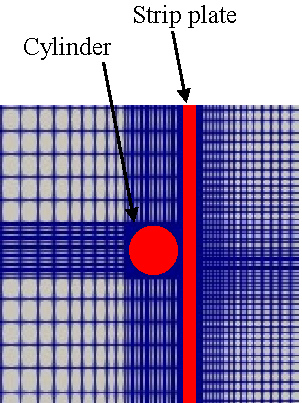
\includegraphics[width=\textwidth]{figs/threeGridsFine}
    % 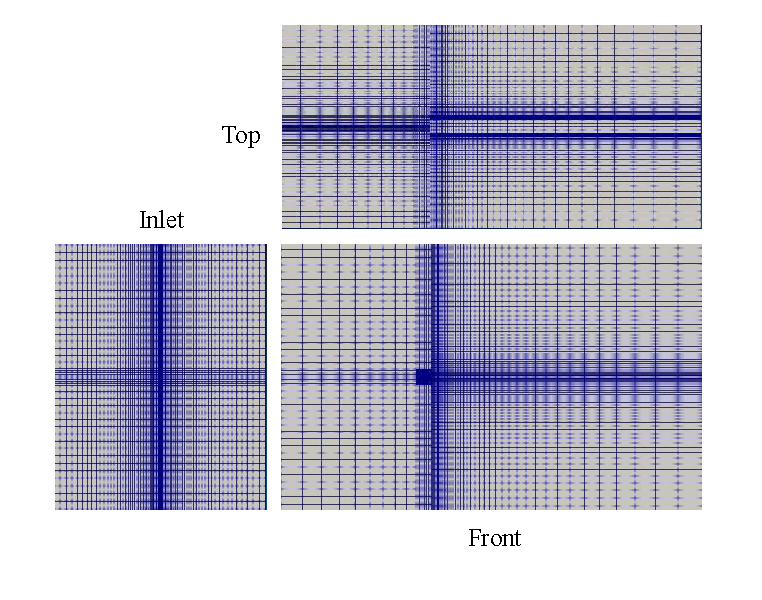
\includegraphics[width=\textwidth]{figs/figure6c}
    \caption{Fine}
    \label{fig:fineMesh}
  \end{subfigure}

  \caption{The course, medium and fine mesh used in the grid independency study.} \label{fig:threeGrids}
\end{figure}


With $v_{i}$ as the volume of the $i^{\text{th}}$ cell in the grid, and $N$ the total number of cells in the domain, the average cell size becomes

\begin{equation}
  h = \frac{1}{N} \left [ \sum_{i=1}^{N} v_{i} \right ]^{1/3},
  \label{eq:averageCellSize}
\end{equation}

\noindent and the normalised average cell size is hence

\begin{equation}
  h/D = \frac{1}{ND} \left [ \sum_{i=1}^{N} v_{i} \right ]^{1/3}.
  \label{eq:normAveCellSize}
\end{equation}

Let $f_{1},f_{2},f_{3},\dots,\fk$ be the quantity of interest obtained from several grid resolutions. A larger subscript is assigned for a coarser grid, thus ascribing $f_{1}$ to the finest and $\fk$ to the coarsest grid. Let the difference between successive solutions be $\epsilon_{2,1},\epsilon_{3,2},\epsilon_{4,3},\dots,\epsilon_{n,n-1}$, where $\epsilon_{2,1} = f_{2} - f_{1}$, $\epsilon_{3,2} = f_{3} - f_{2}$ and so on. Then, the GCI is computed as

\begin{equation}
  \text{GCI}_{i+1,i} = F_{s} \frac{\left |\epsilon_{i+1,i} \right |}{f_{i} \left ( r^{p} - 1 \right )} \times 100\%,
  \label{eq:gci}
\end{equation}

\noindent where $F_{s}$, $f_{i}$ and $r^{p}$ denotes the safety factor $\left ( = 1.25 \right )$, quantity of interest and the refinement ratio, $r$, between successive grids raised to the order of accuracy of the series of solution, $p$. The limit of the solution can be estimated by decreasing the spacing between grid points, allowing it to approach zero via the $\text{p}^{\text{th}}$ method. In essence, the generalised Richardson extrapolation of the quantity of interest is computed as follows.

\begin{equation}
  \fre = f_{1} + \frac{f_{1} - f_{2}}{\rp - 1},
  \label{eq:richardsonExtrapolation}
\end{equation}

\noindent where $\fre$ is the Richardson extrapolation of the quantity of interest. Using $\fre$ to estimate the limit of the monotonically convergent series of $f_{i}$, one can determine the percentage difference of the solution on the finest grid from this limit as

\begin{equation}
  E_{i} = \frac{f_{i} - \fre}{\fre} \times 100\%.
  \label{eq:percentageDifference}
\end{equation}

\section{Chapter Summary} \label{sec:chapSumMethod}
This chapter covers the methods employed to attain the objectives outlined in Chapter One. A cruciform consisting of an upstream circular cylinder and a strip plate placed $G=0.16D$ downstream is the design geometry studied in this thesis and the primary mode of investigation is numerical, i.e., using CFD. The numerical model is solved using OpenFOAM, which is used to discretise the continuity and the RANS form of the momentum transport equation. The turbulence model employed is the one-equation Spalart-Allmaras model, which has been shown time and again in the literature to capture the essence of the flow in VIV situations. The arbitrarily coupled mesh interface (ACMI) allows the mesh quality to be preserved.

The experimental method used to validate the CFD setup consists of an elastically supported cruciform oscillator in an open flow channel. The side plates supporting the two ends of the upstream circular cylinder are marked with a visual marker, thus enabling their motion to be tracked and the displacement time series obtained using a motion capture camera and a motion tracking software.

The phase lag between the lift and vibration signals is computed using the Hilbert-Huang transform. This is done by averaging the instantaneous phase difference between two characteristic components for lift and vibration after the application of HHT. The characteristic component for vibration is the one with largest root-mean-square amplitude. The characteristic component for lift is the one with the highest correlation to the characteristic component of vibration. Computation of fluid and mechanical power is shown to be dependent on $\plag$ and $\fcyl$. Both $\plag$ and $\fcyl$ come from the results of the HHT analysis.

Finally, the chapter outlined the method to gauge the independency of numerical solutions against spatial discretisation. The parameters are then plotted in the next chapter to demonstrate the convergence of the quantities of interest, i.e., $\ystr$, $\fstr$, and Cl. In the next chapter, the thesis discusses the results of the grid independency study and then details the results of this research.

\chapter{Results and Discussion} \label{chap:resultsDisc}

This chapter presents the results and discussion of the data collected using the methods outlined in Chapter Three. First, the results of the benchmarking of the experimental apparatus is shown and discussed. This is followed by a discussion on the grid convergence index study to establish the reliability of the numerical results. Then, the chapter presents the results for the pure cruciform, steep-angled cruciforms ($67.5 \si{\degree}$ and $45 \si{\degree}$) and shallow angled cruciforms ($22.5 \si{\degree}$ and $0 \si{\degree}$). Each of the sections on pure, steep and shallow cruciforms discuss the respective results following the methodology summarised in Fig. \ref{fig:flowChartB}, under the procedure to fulfil objectives one and two. This means that the system response is discussed first, followed by explanations on the system responses based on the observed vortical structures. Finally, the results on the exploration of the $\alpha \; (\si{\degree})-\ured$ parameter space, in terms of vibration amplitude, power and efficiency is presented and discussed to achieve objective three.

\section{Experimental Apparatus Benchmarking} \label{sec:appBenchmark}

 Following the procedure to set the freestream velocity in Section \ref{sec:openFlowExp}, the velocity of the flow at different input voltages are sampled by the voltage controller, the final product being an input voltage $V_{\text{in}}$ (V) versus centreline velocity $U_{\text{cent.}}$ calibration curve. This calibration curve allows the setting of the freestream velocity of the open flow channel by specifying the input voltage to the pump. The finished product gave an operability range between \uth{} and \uel{}, which translates to $\urth \leq \ured \leq \urel$ for an circular cylinder of diameter \SI{10}{\milli\metre}. The turbulence level ranges between $5\%$ to $8\%$ when the freestream velocity $U_{\infty} \geq \uei$.

 A sample of the normalised displacement -- $\ystr = y/D$ -- measured as a function of time is illustrated in Fig. \ref{fig:sampTimeHist}. This time series allows this work to also compute the normalised cylinder vibration frequency, $\fstr = \fcyl/\fn$ ($\fcyl$ being the vibration frequency of the cylinder). The $\ystr$ data presented in Fig. \ref{fig:sampTimeHist} returns $\ystr = 0.33 \pm 0.03$ and $\fstr = 1.03 \pm 0.04$, after computing the uncertainty from multiple experimental runs. In their work, \citet{Koide2013} obtained $\ystr = 0.32$ and $\fstr = 1.09$ at a similar $\ured$ - values that are well within the measurement uncertainty of the experiment. This provides a basis for the reliance on results obtained from the experimental system later in the study.

\begin{figure}[!h]
  \centering
  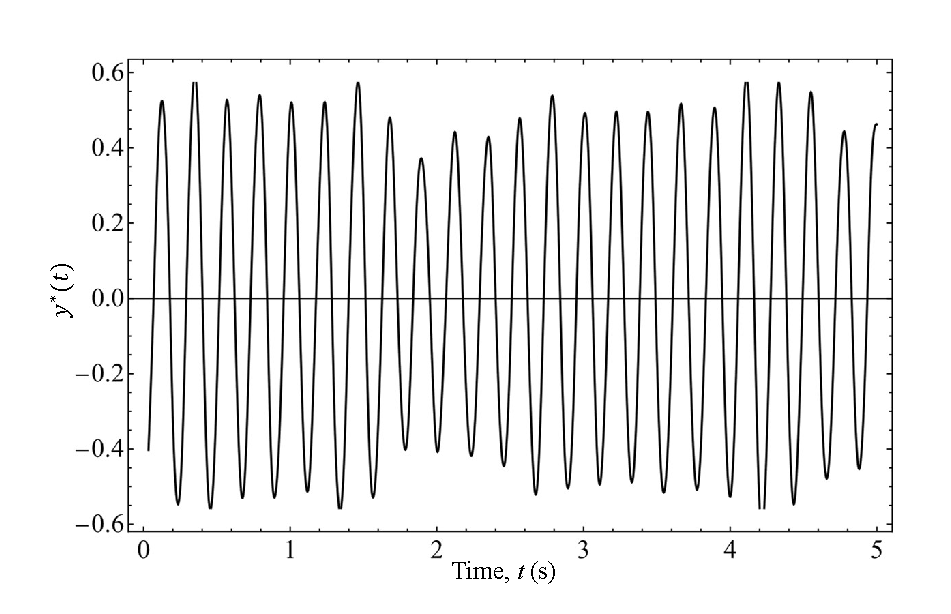
\includegraphics[width=1\textwidth]{figs/figure5}
  \caption{Experimentally measured $y^{*}(t)$, which is the normalised cylinder displacement time series.}
  \label{fig:sampTimeHist}
\end{figure}

\section{The Grid Convergence Index Study} \label{sec:gciStudyResult}

Table \ref{tab:gridIndependency} summarises the result of the grid convergence index (GCI) study for the pure cruciform at reduced velocity $\ured = 22.7$. The flow global quantities checked for convergence are the vibration amplitude $\yrms$, vibration frequency $\fstr$ and lift coefficient $\clrms$ of the cylinder. Both $\yrms$ and $\clrms$ in Fig. \ref{fig:gciRichardson} have initial values smaller than their Richardson extrapolations, $\fre$, before approaching $\fre$, with decreasing $h$. The vibration frequency, on the other hand, starts at a value larger than its $\fre$ before approaching $\fre$.

\begin{table}[!ht]
\centering
\caption{Summary of grid independency study.} \label{tab:gridIndependency}
\vspace{\baselineskip}
\setlength{\tabcolsep}{10pt}      % This is the table column padding. Default value: 6pt
\renewcommand{\arraystretch}{1.5} % This is the table row padding. Default value: 1
\begin{tabular}{l c c c}
  \hline
  \hline
Parameter/ metric                                                       & $\clrms$       & $\yrms = \ystr/D$ & $\fstr = \fcyl / \fn$ \\
  \hline
$\fre$                                                                  & $0.262$        & $0.369$           & $0.969$               \\
$f_{1}$                                                                 & $0.2598$       & $0.3687$          & $0.9695$              \\
$f_{2}$                                                                 & $0.2430$       & $0.3588$          & $0.9740$              \\
$f_{3}$                                                                 & $0.0805$       & $0.2374$          & $1.0220$              \\
$\left | \epsilon_{2,1} \right |$                                       & $0.02$         & $0.01$            & $0.004$               \\
$\left | \epsilon_{3,2} \right |$                                       & $0.16$         & $0.12$            & $0.48$                \\
$R = \left | \epsilon_{2,1} \right | / \left | \epsilon_{3,2} \right |$ & $0.10$         & $0.08$            & $0.094$               \\
$\text{GCI}_{3,2}$                                                      & $30.92$        & $6.00$            & $0.64$                \\
$\text{GCI}_{2,1}$                                                      & $1.63$         & $0.52$            & $0.10$                \\
  \hline
  \hline
\end{tabular}
\end{table}

The most significant drop in GCI is experienced by $\clrms$, with increasing refinement of the grid. Refinement from the coarse to medium grid returns a GCI of $30.92\%$. The GCI of $\clrms$ decreases further to $1.63\%$ with further refinement of the grid. On the other hand, GCI for $\fstr$, shrinks to about one-sixth of its former value.
% , using a refinement ratio of $1.376$. The refinement ratio is computed by dividing the number of cells in one grid with the grid one stage refined. Generalising this to $i$ number of grids returns

Inspecting Fig. \ref{fig:gciRichardson}, the quantities of interest is found to be very close to its Richardson extrapolation at the fine grid (grid 1) for all $\clrms$, $\yrms$ and $\fstr$. This seems to be an indication of sufficient spatial discretisation. At this point, the trade-off between a solution even closer to the Richardson extrapolation and the increased computational effort is no longer appealing, compounded by the observation that values of $\yrms$ and $\fstr$ at the fine grid already falls within the experimental uncertainty as evidenced by measurements in Section \ref{sec:appBenchmark} and the work by \citet{Koide2013}.

% \begin{figure}
%   \centering
%   \begin{subfigure}[h]{1\textwidth}
%     \hspace{2.4cm}
%     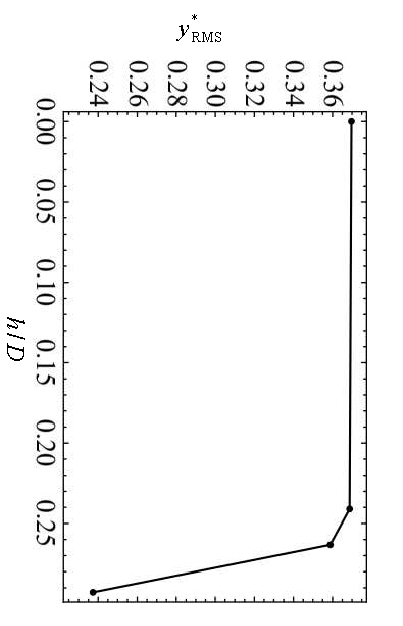
\includegraphics[angle=90,width=0.6\textwidth]{figs/gciYrms-1a}
%     \caption{}
%     \label{fig:gciYrms-1}
%   \end{subfigure}

%   \begin{subfigure}[h]{1\textwidth}
%     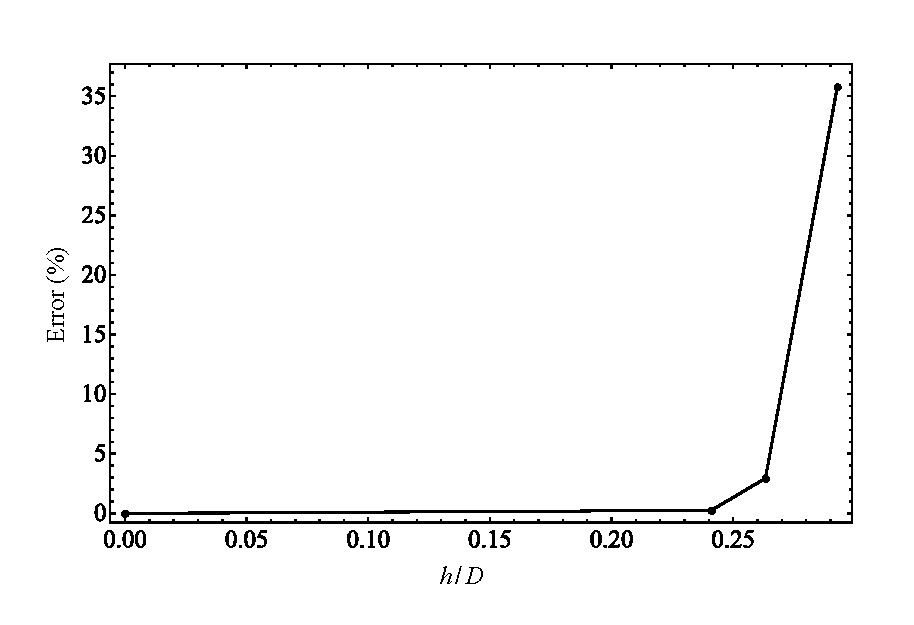
\includegraphics[width=\textwidth]{figs/gciYrms-2}
%     \caption{}
%     \label{fig:gciYrms-2}
%   \end{subfigure}

%   \caption{Richardson extrapolation of $\yrms$ and the corresponding drop in error.} \label{fig:gciYrms}
% \end{figure}
\begin{figure}
  \centering
  \begin{subfigure}[h]{1\textwidth}
    \hspace{1.9cm}
    \includegraphics[angle=90,width=0.7\textwidth]{figs/gciYrms-1a}
    \caption{}
    \label{fig:gciYrms-1}
  \end{subfigure}

  \begin{subfigure}[h]{1\textwidth}
    \hspace{1.9cm}
    \includegraphics[angle=90,width=0.7\textwidth]{figs/gciFstr-1a}
    \caption{}
    \label{fig:gciFstr-1}
  \end{subfigure}

  \begin{subfigure}[h]{1\textwidth}
    \hspace{1.9cm}
    \includegraphics[width=0.7\textwidth]{figs/gciClrms-1a}
    \caption{}
    \label{fig:gciClrms-1}
  \end{subfigure}
  \caption{Richardson extrapolation of $\yrms$, $\fstr$ and $\clrms$.} \label{fig:gciRichardson}
  % \caption{Richardson extrapolation of $\yrms$, $\fstr$ and $\clrms$.} \label{fig:gciYrms}
\end{figure}

% \begin{figure}
%   \centering
%   \begin{subfigure}[h]{1\textwidth}
%     \includegraphics[width=\textwidth]{figs/gciFstr-2}
%     \caption{}
%     \label{fig:gciFstr-2}
%   \end{subfigure}
%   \caption{Richardson extrapolation of $\fstr$ and the corresponding drop in error.} \label{fig:gciFstr}
% \end{figure}

% \begin{figure}
%   \centering
%   \begin{subfigure}[h]{1\textwidth}
%     \includegraphics[width=\textwidth]{figs/gciClrms-2}
%     \caption{}
%     \label{fig:gciClrms-2}
%   \end{subfigure}
%   \caption{Richardson extrapolation of $\clrms$ and the corresponding drop in error.} \label{fig:gciClrms}
% \end{figure}

As demonstrated by the GCI study, $\ystr$, $\fstr$, $\clrms$ all converge as the mesh is refined. This is apparent through the computation of the Richardson extrapolation of each quantity, in addition to the GCI values that drop significantly with each subsequent refinement of the mesh. Furthermore, the error between the values of $\ystr$, $\fstr$ and $\clrms$ and their corresponding Richardson extrapolation also decreases asymptotically to zero, as shown in Fig. \ref{fig:richardsonError}. Now that the independency of the quantities of interest has been established, the chapter will proceed to present results for the pure cruciform in the next section.

\begin{figure}[!h]
  \centering
  \hspace{1cm} \includegraphics[width=0.7\textwidth]{figs/richardsonError}
  \caption{The error between the values of $\ystr$, $\fstr$ and $\clrms$ and their corresponding Richardson extrapolation.}
  \label{fig:richardsonError}
\end{figure}

\section{The pure cruciform}\label{sec:svivRegime}
% This section details the investigations conducted with regards to the pure cruciform in terms of it being the oscillator in an energy harvesting system. The pure cruciform serves as the base upon which all subsequent results will be compared against.
% The reason behind it being the base reference lies in the expansiveness of studies done, making it the type of cruciform oscillator that is most known about. Recall that it is through the study of the pure cruciform oscillator that the three main merits of the cruciform oscillator becomes known: a highly adept passive control system via the downstream strip plate, a very wide synchronisation range, and an approximately constant maximum vibration amplitude across the synchronisation range \citep{Koide2013}.

% Despite this, in recent years, improvement in terms of power output from the pure cruciform system seems to have hit a wall. Part of the reason behind this engineering roadblock is the fact that studies on pure cruciform oscillators to date have been focussed on answering the ``what happens if'' questions instead of the ``why'' questions concerning its system response. This work is of the opinion that if the roadblock is to be removed, efforts must be made to answer the ``why'' questions and the first step towards that is by understanding why does one observe the system responses found in the literature. This is possible through the use of CFD as one can quite effortlessly make simultaneous measurements of the cylinder displacement and lift while also obtain quantitative visualisations of the three-dimensional flow field describing the vortical structures governing the vibration of the cylinder.

% The roadblock can also be interpreted as a sign to apply new methods of analysis on the common signals that are studied during the course of a VIV study, which are the time series of cylinder displacement and lift. Coupled with quantitative visualisations of the dominant vortical structures in the flow, this thesis attempts to look for clues that can guide future designs of the cruciform system as an energy harvester and bring to the table knowledge beyond improving its power output and efficiency, but the ability to control them, and adapting them to suit the natural environment within which the cruciform oscillator harnesses energy. This is because, even if the engineering knowledge allows for the vibration amplitude and frequency to reach a certain maximum value - and thus power - within a range of flow velocities, the aquatic or marine environment it is submitted to may not be suitable for such deployments, especially when faced with aquatic and marine life protection responsibilities \citep{Raghavan2007a}.

The section starts by reproducing the amplitude/frequency responses of the pure cruciform, followed with the investigation of the vortical structures that bring about the amplitude/frequency responses observed. Then, the Hilbert-Huang transform is applied to elucidate the temporal evolution of the phase angle between lift and cylinder displacement to discover potentially hidden branches in the amplitude response not previously subjected to energy harvesting. Finally, the section concludes with the decomposition of the lift signal and the discovery of clues to maximise the vibration-driving lift, and consequently vibration amplitude and power output.

\subsection{The amplitude and frequency response}\label{ssec:svivRegimeAmpFreqResp}

The pure cruciform case, i.e. \angfi{}, demonstrated a normalised \rms{} amplitude of cylinder displacement, $\yrms$ that starts quite expectedly with a low amplitude at reduced velocities $\uron$ and $\urtw$ , before reaching a value close to $\yrms = 0.1$ at $\ured = \urth$, as presented in Fig. \ref{fig:yStrRMS1}. Following the local maximum at $\ured = \urth$, $\yrms$ tapers off to less than $\yrms = 0.05$ between $\urfo \leq \yrms \leq \ursi$. This whole $\yrms$ trend of hitting a local maximum before tapering off bears a striking resemblance to the amplitude response of an isolated circular cylinder in KVIV at mass ratios of order $O(10^{1})$ \citep{Feng1963,Khalak1999}. This resemblance can be seen as an indication that the vibration of a pure cruciform between $\ured \leq \urse$ is driven primarily through the shedding cycle of Karman vortices.

\begin{figure}
  \centering
  \includegraphics[width=1\textwidth]{figs/yStrRMS1}
  \caption{Evolution of the normalised \rms{} amplitude of cylinder displacement $\yrms$, with respect to reduced velocity $\ured$, in the streamwise vortex-driven vibration regime.} \label{fig:yStrRMS1}
\end{figure}

Then at $\ured = \urse$, $\yrms$ experiences a very weak increase followed by a sudden jump close to $0.4$ at $\ured = \urei$. This is followed by a slight decline at $\ured = \urni$ and return to the previous level of $\yrms$ at $\ured = \urte$. Past $\ured = \urte$, one observes that $\yrms$ maintains a linear trend in its variation with respect to $\ured$. As $\ured = \urei$ is well within the lower branch for a system in KVIV, it is quite unlikely for the vibration within $\urei \leq \ured \leq \urtt$ to be the governed by the shedding of Karman vortices, leading previous investigators to attribute the vibration to the periodic shedding of streamwise vortical structures dominating the spatial region close to the cruciform juncture \citep{Shirakashi1989,Hemsuwan2018b,Hemsuwan2018d}. Hence, this range is named of $\ured$ the streamwise vortex-induced vibration regime (SVIV).

\begin{figure}
  \centering
  \includegraphics[width=1\textwidth]{figs/expCompareAmp}
  \caption{Comparison between the evolution of $\yrms$ with respect to $\ured$of a pure cruciform system from the numerical and experimental work. The filled square represents the numerical, while the filled circle represents the experimental results.}
  \label{fig:expCompareAmp}
\end{figure}

The experimental system consisting of the closed loop open flow channel and the pure cruciform oscillator rig in Section \ref{sec:openFlowExp} is constructed not only for the purpose of validating the results of the pure cruciform numerical investigation, but also to corroborate in general, the sum total of the numerical setup. Admittedly, the best undertaking would be to perform equivalent experiment for each of the \angfi{}, \angfo{}, \angth{}, \angtw{} and \angon{} configurations, but the scale of such an exercise and subsequent discussion of the results in the opinion of this work, deserves its own treatment separate from the current study. The degree of agreement between the results of the numerical and experimental investigation of the pure cruciform establishes the validity of the numerical setup, which is taken as extending to the rest of the cruciforms. This assumption is somewhat founded because all cruciforms are simulated under similar boundary conditions, mesh resolution and solver algorithm.

The experiments collect time series data of cylinder displacement $y$, from which the normalised \rms{} amplitude $\yrms$ is computed. Figure \ref{fig:expCompareAmp} compares both numerical and experimental results of $\yrms$. Both results agree in terms of magnitude and trend of the amplitude response. However, the jump to SVIV occurs at a higher $\ured \approx 19$, translating to a delay of about 3 units of $\ured$. The numerical and experimental results are also able to capture the slight dip in $\yrms$ following the jump to SVIV, but the occurrence in the experiment is also delayed by about 3 units of $\ured$. This delay can perhaps be attributed to the fact that the raw $y$ time series were measured in succession from the lowest attainable channel flow velocity \uth{} to its highest \uel{} within one experimental run. In contrast, the simulations always start with the cylinder at rest at its neutral position at $t_{0} = \SI{0}{\second}$, with the freestream exactly at set at the desired value $\uon, \utw, \dots, \utt$. Thus, the delays found in experimental results may simply be the consequence of ``flow memory'', a concept whose analogy can be found in experiments concerned with the critical value of a nondimensional quantity, e.g. Reynolds number, that demarcates the transition between two states of flow \citep{Saint-Michel2014,Rahman2015,Li2021}. For all practical purposes, ``flow memory'' is simply the natural tendency of a fluid to retain its current state of flow for as long as it can, before being altered by an increase/decrease in momentum. This results in the delay found at the jump to SVIV and the local $\yrms$ minimum after the jump.

\begin{figure}
  \centering
  \includegraphics[width=1\textwidth]{figs/yStrFreq5}
  \caption{Evolution of the normalised cylinder displacement frequency, $\fstr$, with respect to reduced velocity $\ured$, for the pure cruciform case.}
  \label{fig:yStrFreq5}
\end{figure}

The evolution of the normalised cylinder vibration frequency $\fstr$ with respect to $\ured$ is shown in Fig. \ref{fig:yStrFreq5}. Inspecting Fig. \ref{fig:yStrFreq5}, one immediately notice two distinct evolutionary pattern for $\fstr$with a sharp boundary at $\ured = \ursi$. Between $\uron \leq \ured \leq \ursi$, the $\fstr$ trend follows closely the shedding frequency of Karman vortices from an isolated, fixed circular cylinder \citep{Blevins1990}. The Karman vortex shedding frequency is given as an empirical equation in Eq. \ref{eq:karmanSheddingFreq}.

\begin{equation}
  \fvk = 0.198 \left( 1 - \frac{19.7}{\re} \right) DU
  \label{eq:karmanSheddingFreq}
\end{equation}

\noindent Here, $\fvk$, $D$ and $U$ are the vortex shedding frequency, diameter of the isolated circular cylinder and $U$ the freestream velocity respectively. One can easily see how $\fvk$ is a linear function of $U$, and this is what gives rise to the linear pattern of $\fstr$ within $\uron \leq \ured \leq \ursi$. Then, within $\urse \leq \ured \leq \urtt$, $\fstr$ drops close to 1, indicating synchronisation between lift and cylinder vibration. It seems that this synchronisation is what gives rise to the bigger $\ystr$, compared to $\uron \leq \ured \leq \ursi$.

Inspecting the evolution of \rms{} amplitude of lift coefficient $\clrms$ and the normalised lift coefficient frequency $\fclstr$ with respect to $\ured$ in Fig. \ref{fig:cl90}, provided more evidence supporting the assertion that $\ured = \urse$ is a boudary berween two vibration-driving mechanisms. In fact, the observation at $\urse$ in Fig. \ref{fig:clRMS5} indicates that the SVIV regime is still in its infancy, due to the dip in $\clrms$ at that $\ured$, compared to $\ured = \ursi$. In Fig. \ref{fig:clFreq5}, a dashed line is also drawn to illustrare $f^{*}_{v} = \fvk/D$, where $\fvk$ is the shedding frequency of Karman vortices from a smooth isolated circular cylinder described in Eq. \ref{eq:karmanSheddingFreq}.

The trend found in $\fclstr$ vs. $\ured$ is very similar to that found in Fig. \ref{fig:yStrFreq5}. This similarity is interpreted as an indication of the symmetry of lift produced along the cylinder. This reasoning stems from the findings of \citet{Zhao2018a}, who revealed how lift is distributed along the upstream cylinder of a two-cylinder \angfi{} cruciform. They did this by computing chapteral lift coefficients along the upstream cylinder. This system produces a symmetric distribution of chapteral lift coefficient, with $Z = 0$ being the plane of symmetry. An asymmetrical distribution of the chapteral lift coefficient may produce a trend in $\yrms$ and $\fstr$ that is dissimilar to those found in $\clrms$ and $\fclstr$, due to the irregular moment acting on the cylinder.

\begin{figure}
  \centering
  \begin{subfigure}[h]{1\textwidth}
    \includegraphics[width=\textwidth]{figs/clRMS5}
    \caption{Evolution of $\clrms$ with respect to $\ured$.}
    \label{fig:clRMS5}
  \end{subfigure}

  \begin{subfigure}[h]{0.95\textwidth}
    \includegraphics[width=\textwidth]{figs/clFreq5}
    \caption{Evolution of $\fclstr$ with respect to $\ured$}
    \label{fig:clFreq5}
  \end{subfigure}

  \caption{Evolution of the lift coefficient \rms{} amplitude ($\clrms$) and normalised frequency of lift coefficient ($\fclstr$), with respect to reduced velocity $\ured$, for the pure cruciform case. The dashed line in Fig. \ref{fig:clFreq5} visualises the shedding frequency of Karman vortex computed from Eq. \ref{eq:karmanSheddingFreq}.} \label{fig:cl90}
\end{figure}

\subsection{Main vibration-driving vortical structure}\label{ssec:svivRegimeVortStruct}
Recall Figs. \ref{fig:yStrRMS1} and \ref{fig:yStrFreq5}. Out of all thirteen variants of $\ured$ studied in the pure cruciform case, seven within $\urse \leq \ured \leq \urtt$ sustain high-amplitude vibrations with no foreseeable upper limit within the observation window. For a more complete understanding of the mechanism driving the vibration, one needs to know what are the vortical structures dominating the flow are and how they interact with each other.

\begin{figure}
  \centering
\includegraphics[width=1\textwidth]{figs/probe90YU10}
\caption{Distribution of normalised frequency of vortex shedding, along the span of the cylinder of the pure cruciform at $\ured = \urte$.}
  \label{fig:probe90YU10}
\end{figure}

Let the coordinates of the simulation domain be defined in the following manner: $\left( X, Y, Z \right) = \left( \frac{x}{D}, \frac{y}{D}, \frac{z}{D} \right)$. The $y$-component velocity fluctuations are sampled on the $\left ( X, Y \right ) = \left ( 1.96, 0 \right )$ line, along the span of the cylinder in $0.5D$ increments, i.e. at coordinates $\left ( 1.96, 0, 7.5 \right )$, $\left ( 1.96, 0, 7.0 \right )$, \dots, $\left ( 1.96, 0, -7.5 \right )$. The distance $X = 1.96$ from the origin is equivalent to $1D$ downstream the trailing edge of the strip plate, and this location is chosen as it is not too close to the cruciform that the vortical structures have not fully formed, and not too far, obfuscating meaningful observation of the structures.

The shedding of vortical structures leave their footprint on the flow field in the form of velocity fluctuations. The choice of analysing the fluctuations of the $y$-component of velocity is made due to the fact that the oscillator is constrained to move only in the transverse direction. Then, the velocity fluctuations are processed with FFT to obtain the Fourier transform of the fluctuation signals at each spanwise location. The combines Fourier transforms are presented using a colour map in Fig. \ref{fig:probe90YU10}. In this figure, every point is a result of that FFT giving the observer a spatial understanding of the vortical structures present in the flow. The abscissa and ordinates denotes $\fstr$ and $Z$ coordinates respectively, while the bar legend gives the amplitude of the FFT result.

Through inspection, one immediately notices two frequency bands with high amplitudes namely $\fstr \approx 1$ and $\fstr \approx 4.5$. The locations of these bands are between $3 \leq Z \leq 4.5$ for the former and $4.5 < Z \leq 7$ for the latter. Aided with this visualisation, one can give meaning to the $x$ and $z$-components of vorticity visualised in Fig. \ref{fig:vortStruct90} . The slices in Fig. \ref{fig:vortStruct90} visualise the distribution of the $x$ (streamwise) and $z$ (Karman) components of vorticity at the $X = 1.96$ plane. The plane is viewed from downstream (viewer standing at $X = 1.96$, looking towards the cruciform), and the vorticites are presented in units of \si{\per\second}. Furthermore, the visualisations are made when the lift coefficient $\cl$ is at a maximum ($\text{Cl}_{\text{max}}$).

Comparing Fig. \ref{fig:probe90YU10} with Fig. \ref{fig:vortStruct90} suggests that the $\fstr \approx 1$ band is actually due to the shedding of streamwise vortex of a scale close to $1D$ while the $\fstr \approx 4.5$ seems to be due to the shedding of Karman vortices. Contrary to the vortical structure commonly observed in studies of isolated circular cylinders \citep{Deng2007,Kinaci2016,Duranay2020}, in the pure cruciform case, two distinct vortical structures take shape in the flow, namely streamwise and Karman vortices. This is consistent with the findings in \citet{Koide2017} or \citet{Zhao2018a}, where they observed a pair of streamwise vortices on a scale of $\approx 1D$ form in the vicinity of the cruciform juncture, and Karman vortices further away in the spanwise direction. Note that the vibration-driving streamwise vortices forming close to the cruciform juncture exist in pairs: in Fig. \ref{fig:vorx90}, one is observed to rotate in the clockwise direction when $Z > 0$ and the other in the counter-clockwise direction when $Z < 0$. What results from this counter-rotating vortex pair is a thrust, propelling the cylinder upwards. This is consistent with the fact that the vorticity field visualisations are produced when the $\cl$ is at a maximum. This work also observe the core of both streamwise vortices lie approximately on the same $Y$-plane, parallel to the axis of the cylinder.

\begin{figure}
  \centering
  \begin{subfigure}[h]{0.7\textwidth}
    \includegraphics[width=\textwidth]{figs/vorx90}
    \caption{$x$-component vorticity}
    \label{fig:vorx90}
  \end{subfigure}

  \begin{subfigure}[h]{0.7\textwidth}
    \includegraphics[width=\textwidth]{figs/vorz90}
    \caption{$z$-component vorticity}
    \label{fig:vorz90}
  \end{subfigure}

  \caption{Dominant vortical structures at $\ured = \urte$ observed in the pure cruciform case.} \label{fig:vortStruct90}
\end{figure}

\begin{figure}
  \centering
  \begin{subfigure}[h]{0.9\textwidth}
    \includegraphics[width=\textwidth]{figs/qIso090U10}
    \caption{Isometric view of the Q-criterion.}
    \label{fig:qIso090U10}
  \end{subfigure}
  
  \begin{subfigure}[h]{0.9\textwidth}
    \includegraphics[width=\textwidth]{figs/qTop090U10}
    \caption{Plan view of the Q-criterion.}
    \label{fig:qTop090U10}
  \end{subfigure}

  \caption{The Q-criterion for the 90$^{\circ}$ cruciform at $\ured = \urte$: the isometric (\ref{fig:qIso090U10}) and plan view (\ref{fig:qTop090U10}).} \label{fig:qCrit090U10}
\end{figure}

\begin{figure}
  \centering
  \begin{subfigure}[h]{0.9\textwidth}
    \includegraphics[width=\textwidth]{figs/qIso090U02}
    \caption{Isometric view of the Q-criterion.}
    \label{fig:qIso090U02}
  \end{subfigure}
  
  \begin{subfigure}[h]{0.9\textwidth}
    \includegraphics[width=\textwidth]{figs/qTop090U02}
    \caption{Plan view of the Q-criterion.}
    \label{fig:qTop090U02}
  \end{subfigure}

  \caption{The Q-criterion for the 90$^{\circ}$ cruciform at $\ured = \urth$: the isometric (\ref{fig:qIso090U02}) and plan view (\ref{fig:qTop090U02}).} \label{fig:qCrit090U02}
\end{figure}

\subsection{Temporal evolution of the lift coefficient} \label{ssec:tempEvo}
As one can see from the previous section, the streamwise vortex-induced vibration energises the oscillation of the cylinder from within the lower branch of KVIV. However, the amplitude response seems to only increase slightly with each increase of $\ured$, bordering on tapering off. This is different from oscillators that operate in the galloping mode, which exhibits a perceptible increase for as long as the reduced velocity $\ured$ is increased. The following sections attempt to uncover the reason for this observation, which can help to improve the power output in subsequent iterations of the cruciform energy harvester by investigating the temporal evolution of the lift coefficient.

\subsubsection{The KVIV regime (reduced velocity below 13.6)} \label{sssec:phaseLag}
%% Paraphrase in Grammarly BEGIN
At reduced velocities  $\ured = 2.3$ and 4.5, the phase lags  $\phi$ (deg.) between $\cl$ and  $\ured$ are practically zero throughout the whole observation time. The characteristic intrinsic mode functions (IMFs) of $\cl$ and  $\ystr$ at $\ured = 4.5$ exemplifies this trend, as showcased in Fig. \ref{fig:tempAnalysisKVIV}. Here, Fig. \ref{fig:tempAnalysisKVIV}a shows the temporal evolution of $\cysys$ and $\cclys$, which are the characteristic IMFs of $\ystr$ and Cl, respectively. Figure \ref{fig:tempAnalysisKVIV}b shows the phase lag between $\cysys$ and $\cclys$, and Fig. \ref{fig:tempAnalysisKVIV}c presents the Hilbert-Huang transform (HHT) spectrogram of Cl. The HHT spectrogram visualises the instantaneous frequency and amplitude of the decomposed $\cl$ signal. The trend in Fig. \ref{fig:tempAnalysisKVIV}b is similar to what was observed by \citet{Khalak1999} which also employs the Hilbert transform to compute the instantaneous phase. It is worth noting that the signals dealt with in \citet{Khalak1999} are more or less monotonic, rendering empirical mode decomposition (EEMD) irrelevant. The dominant IMF component of the lift coefficient has a normalised frequency $\fclstr = f_{\text{Cl}}/\fn$ (Fig. \ref{fig:tempAnalysisKVIV}c) centred at approximately $\fclstr = 0.75$. Here, the dominant IMF component refers to the component of IMF with the highest amplitude during the whole observation time.

\begin{figure}
  \centering
  \begin{subfigure}[h]{1\textwidth}
    \includegraphics[width=\textwidth]{figs/tempAnalysisKVIV-a}
    \caption{}
    \label{fig:tempAnalysisKVIV-a}
  \end{subfigure}

  \begin{subfigure}[h]{1\textwidth}
    \includegraphics[width=\textwidth]{figs/tempAnalysisKVIV-b}
    \caption{}
    \label{fig:tempAnalysisKVIV-b}
  \end{subfigure}

  \caption{Temporal analysis of $\cl$ and $\ystr$ at $\ured = \urtw$.}
\end{figure}

\begin{figure} \continuedfloat
  \centering
  \begin{subfigure}[h]{1\textwidth}
    \includegraphics[width=\textwidth]{figs/tempAnalysisKVIV-c}
    \caption{}
    \label{fig:tempAnalysisKVIV-c}
  \end{subfigure}

  \caption{Temporal analysis of $\cl$ and $\ystr$ at $\ured = \urtw$.} \label{fig:tempAnalysisKVIV}
\end{figure}

Once the cylinder enters the upper branch of KVIV at $\ured = 6.8$, $\phi$ jumps to approximately 110 deg. This jump in $\phi$ is commonly observed in the transition to the upper branches \citep{Maruai2018}. Both $\cclys$ and $\cysys$ signals are highly periodic, and the dominant frequency band of $\cl$ is centred at $\approx 1$, as demonstrated in Fig. \ref{fig:tempAnalysisUpper}c.

\begin{figure}
  \centering
  \begin{subfigure}[h]{1\textwidth}
    \includegraphics[width=\textwidth]{figs/tempAnalysisUpper-a}
    \caption{}
    \label{fig:tempAnalysisUpper-a}
  \end{subfigure}

  \begin{subfigure}[h]{1\textwidth}
    \includegraphics[width=\textwidth]{figs/tempAnalysisUpper-b}
    \caption{}
    \label{fig:tempAnalysisUpper-b}
  \end{subfigure}
  \caption{Temporal analysis of $\cl$ and $\ystr$ at $\ured = \urth$.}
\end{figure}

\begin{figure} \continuedfloat
  \centering
  \begin{subfigure}[h]{1\textwidth}
    \includegraphics[width=\textwidth]{figs/tempAnalysisUpper-c}
    \caption{}
    \label{fig:tempAnalysisUpper-c}
  \end{subfigure}
  \caption{Temporal analysis of $\cl$ and $\ystr$ at $\ured = \urth$.} \label{fig:tempAnalysisUpper}
\end{figure}

As $\ured$ is increased even further up to $\ured = \ursi$, a similar trend is spotted for all $\ured = 9.1, 11.4, 13.6$ examined: $\cysys$ and $\cclys$ are both qualitatively very periodic. Their phase lags are very close to $180$ deg. The dominant $\cl$ frequency bands exhibit a time-averaged value that increases linearly for $\ured$ while keeping the Strouhal number of $\cl$ $\approx 0.16$. The representative case of $\ured = \ursi$ is shown in Fig. \ref{fig:tempAnalysisLower}. Note how $\phi$ in this range of $\ured$ varies less against time, compared to $\phi$ at $\ured = \urth$, and the dominant frequency band of $\cl$ is much narrower compared to the dominant frequency band at $\ured = \urth$, indicating a highly periodic and self-similar oscillation of lift.

\begin{figure}
  \centering
  \begin{subfigure}[h]{1\textwidth}
    \includegraphics[width=\textwidth]{figs/tempAnalysisLower-a}
    \caption{}
    \label{fig:tempAnalysisLower-a}
  \end{subfigure}

  \begin{subfigure}[h]{1\textwidth}
    \includegraphics[width=\textwidth]{figs/tempAnalysisLower-b}
    \caption{}
    \label{fig:tempAnalysisLower-b}
  \end{subfigure}
  \caption{Temporal analysis of $\cl$ and $\ystr$ at $\ured = \ursi$.}
\end{figure}

\begin{figure} \continuedfloat
  \centering
  \begin{subfigure}[h]{1\textwidth}
    \includegraphics[width=\textwidth]{figs/tempAnalysisLower-c}
    \caption{}
    \label{fig:tempAnalysisLower-c}
  \end{subfigure}
  \caption{Temporal analysis of $\cl$ and $\ystr$ at $\ured = \ursi$.} \label{fig:tempAnalysisLower}
\end{figure}

\subsubsection{Transition to SVIV (reduced velocity between 15.9 and 18.2)} \label{sssec:transSVIV}
Previously in the $\ured \leq \ursi$ range, the temporal profile of both $\cl$ and  $\ystr$ are very similar, except that $\cl$ leads $\ystr$ by a certain amount. This similarity in profile supports the assertion that the vibration within $\ured \leq \ursi$ is driven exclusively by the shedding of Karman vortices, which brings the onset of the alternating lift. Similarly, a similar profile between $\cl$ and $\ystr$ is expected when streamwise vortices drive the vibration. This presupposition, however, seems to disagree with observation.

Once $\ured$ reaches 15.9, it has become difficult to argue that the profile of $\ystr$ is just a lagged version of the profile of Cl. This is shown in Fig. \ref{fig:tempEvoCompare}a, with the enlarged version in Fig. \ref{fig:tempEvoCompare}b. The profile of $\cl$ is akin to the superposition of a plurality of signals. This observation is driven by the presence of two types of maxima with differing amplitude heights. A red dashed line, and a red dashed-dot line is put in Fig. \ref{fig:tempEvoCompare}b as visual cues indicating the two amplitude heights. Through EEMD, some evidence supporting the compound signal hypothesis is brought to light.

\begin{figure}
  \centering
  \begin{subfigure}[h]{1\textwidth}
    \includegraphics[width=\textwidth]{figs/tempEvoCompare-a}
    \caption{}
    \label{fig:tempEvoCompare-a}
  \end{subfigure}

  \begin{subfigure}[h]{0.98\textwidth}
    \includegraphics[width=\textwidth]{figs/tempEvoCompare-b}
    \caption{}
    \label{fig:tempEvoCompare-b}
  \end{subfigure}
  \caption{Temporal evolution of $\ystr$ and $\cl$ at $\ured = \urse$.} \label{fig:tempEvoCompare}
\end{figure}

Once the signal is decomposed using EEMD, Fig. \ref{fig:tempEvoCompare}a is replotted using $\cclys$ and $\cysys$ in Fig. \ref{fig:tempAnalysisTransition}a. One can clearly see that the part of $\cl$ signal responsible for driving the vibration at  $\ured = 15.9$ is embedded in the original $\cl$ signal (Fig. \ref{fig:tempAnalysisTransition}a), and decomposition via EEMD managed to recover this signal, which leads $\cysys$ by approximately 150 deg. on average, throughout the whole observation time (Fig. \ref{fig:tempAnalysisTransition}b). This decline from $\phi \approx 180$ deg. at reduced velocities $\urfo \leq \ured \leq \ursi$, to $\phi \approx 150$ deg. at $\ured = \urse$ is quite sizeable, suggesting a fundamental change in flow dynamics, particularly in terms of vortical structure. Another significant change is the increased scatter in $\phi$ from its time-averaged value, different from the evolution of $\phi$ in the range $\urfo \leq \ured \leq \ursi$, which varies only slightly throughout the observation time.

\begin{figure}
  \centering
  \begin{subfigure}[h]{1\textwidth}
    \includegraphics[width=\textwidth]{figs/tempAnalysisTransition-a}
    \caption{}
    \label{fig:tempAnalysisTransition-a}
  \end{subfigure}

  \begin{subfigure}[h]{0.98\textwidth}
    \includegraphics[width=\textwidth]{figs/tempAnalysisTransition-b}
    \caption{}
    \label{fig:tempAnalysisTransition-b}
  \end{subfigure}

  \caption{Temporal analysis of the lift coefficient and normalised cylinder displacement signal at $\ured = \urse$.}
\end{figure}

\begin{figure} \continuedfloat
  \centering
  \begin{subfigure}[h]{1\textwidth}
    \includegraphics[width=\textwidth]{figs/tempAnalysisTransition-c}
    \caption{}
    \label{fig:tempAnalysisTransition-c}
  \end{subfigure}
  \caption{Temporal analysis of the lift coefficient and normalised cylinder displacement signal at $\ured = \urse$.}
  \label{fig:tempAnalysisTransition}
\end{figure}

Inspecting the HHT spectrogram in Fig. \ref{fig:tempAnalysisTransition}c reveals two dominant bands in the frequency domain. The first one, denoted by a white rectangular frame, is the instantaneous frequency for the IMF component of lift shown in Fig. \ref{fig:tempAnalysisTransition}a, and its mean frequency lies close to the natural frequency of the system ($\fclstr \approx 1$). Simultaneously, a second frequency band with similar amplitude is marked with a white dashed rectangular frame around $\fclstr \approx 3.3$. The Strouhal number from this frequency is $\st = 0.20$, which is tenuously close to the Strouhal number for Karman vortices as predicted by Eq. \ref{eq:karmanSheddingFreq} for $\re = 7.9 \times 10^{3}$. This second band of frequency is thus attributed to the footprint left by the shedding of Karman vortices and the first band as the result of streamwise vortex shedding. Through visual inspection of Fig. \ref{fig:tempAnalysisTransition}c, both of these dominant frequency bands are markedly wider, and the individual values are more scattered from their time-averaged values than any of their counterparts within $\ured \leq \ursi$.

Observing Karman vortices shedding from a cruciform structure during SVIV is not new in the literature. However, pinpointing how the streamwise and Karman vortex shedding modulates the lift signal from a cruciform structure in SVIV has no precedence. The vibration of the cylinder remains steadfast near the system natural frequency, even though both Karman and streamwise vortices are comparable in terms of amplitude. The underlying cause is probably the shedding frequency of the Karman vortex, which is too distant from the system's natural frequency $\fn$. The shedding frequency of the streamwise vortex is much closer to $\fn$ and is thus preferred by the cylinder.

The transition to SVIV is considered complete at $\ured = 18.2$ when the time-averaged phase lag drops further to $\approx 20$ deg. Figure \ref{fig:tempAnalysisStableInitialBranch}a and \ref{fig:tempAnalysisStableInitialBranch}b documents this observation. The instantaneous phase lag is observed to slip through 360 deg. a little past the two second (\SI{2}{\second}) timestamp. By inspecting Fig. \ref{fig:tempAnalysisStableInitialBranch}a, one finds that a little past \SI{2}{\second} is when distortions in the periodicity of $\cclys$ occur. The slipping through 360 deg. was also mentioned by \citet{Khalak1999} in their work on KVIV, drawing attention to the quasi-periodic nature of the signal. For \citet{Khalak1999}, the slip occurs in the initial branch of KVIV. The overall low value of $\phi$ ($\approx 20$ deg. for the whole observation time at $\ured = 18.2$), coupled with the presence of $\phi$ slippage, is suggestive of the possibility for $\ured = 18.2$ being the initial branch of SVIV.

\begin{figure}
  \centering
  \begin{subfigure}[h]{1\textwidth}
    \includegraphics[width=\textwidth]{figs/tempAnalysisStableInitialBranch-a}
    \caption{}
    \label{fig:tempAnalysisStableInitialBranch-a}
  \end{subfigure}

  \begin{subfigure}[h]{1\textwidth}
    \includegraphics[width=\textwidth]{figs/tempAnalysisStableInitialBranch-b}
    \caption{}
    \label{fig:tempAnalysisStableInitialBranch-b}
  \end{subfigure}
  \caption{Temporal analysis of the lift coefficient and normalised cylinder displacement signal at $\ured = \urei$.}
\end{figure}

\begin{figure} \continuedfloat
  \centering
  \begin{subfigure}[h]{1\textwidth}
    \includegraphics[width=\textwidth]{figs/tempAnalysisStableInitialBranch-c}
    \caption{}
    \label{fig:tempAnalysisStableInitialBranch-c}
  \end{subfigure}
  \caption{Temporal analysis of the lift coefficient and normalised cylinder displacement signal at $\ured = \urei$.}
  \label{fig:tempAnalysisStableInitialBranch}
\end{figure}

\subsubsection{The stable SVIV regime (reduced velocity greater than 20.5)} \label{sssec:svivRegime}
As $\ured$ is increased to 20.5, a jump is observed in $\phi$ from a mean value of approximately 20 deg. to about 120 deg., shown in Fig. \ref{fig:phaseAngle}a. The phase slippage discussed previously is also observed, indicating the quasi-periodic nature of the lift coefficient signal at this $\ured$. Incidentally, this quasi-periodicity seems to be the norm for the lift signals up to $\ured = 27.3$, as suggested by the phase slippages evident in Figs. \ref{fig:phaseAngle}b, c and d. The slippage halts once $\ured$ reaches 29.5, suggesting the emergence of a more periodic lift signal relative to $20.5 \leq \ured \leq 27.3$. Although the instantaneous phase between $20.5 \leq \ured \leq 27.3$ implies a quasi-periodic nature, their time-averaged values at each $\ured$ are contained in the narrow region $114 < \phi$ (deg.) $< 135$, as is the value for $\phi$ at $\ured = 29.5$. This finding can be interpreted as the dominant vortical structures becoming more resilient against external excitations. Hence, $20.5 \leq \ured \leq 29.5$ is classified as the upper branch of SVIV.

\begin{figure}
  \centering
  \begin{subfigure}[h]{1\textwidth}
    \includegraphics[width=\textwidth]{figs/phaseAngle-a}
    \caption{}
    \label{fig:phaseAngle-a}
  \end{subfigure}

  \begin{subfigure}[h]{1\textwidth}
    \includegraphics[width=\textwidth]{figs/phaseAngle-b}
    \caption{}
    \label{fig:phaseAngle-b}
  \end{subfigure}

  \begin{subfigure}[h]{1\textwidth}
    \includegraphics[width=\textwidth]{figs/phaseAngle-c}
    \caption{}
    \label{fig:phaseAngle-c}
  \end{subfigure}

  \begin{subfigure}[h]{1\textwidth}
    \includegraphics[width=\textwidth]{figs/phaseAngle-d}
    \caption{}
    \label{fig:phaseAngle-d}
  \end{subfigure}
  \caption{The instantaneous phase lag $\phi$ of $\cclys$ in the range $\urni \leq \ured \leq \urtt$.}
\end{figure}

\begin{figure} \continuedfloat
  \centering
  \begin{subfigure}[h]{1\textwidth}
    \includegraphics[width=\textwidth]{figs/phaseAngle-e}
    \caption{}
    \label{fig:phaseAngle-e}
  \end{subfigure}
  \caption{The instantaneous phase lag $\phi$ of $\cclys$ in the range $\urni \leq \ured \leq \urtt$.}
  \label{fig:phaseAngle}
\end{figure}

The $\phi(t)$ data makes it possible to visualise the vibration ``branches'' within the $\ured$ range investigated. As the branches are mapped against $\ured$, a representative value of $\phi$ is needed at each $\ured$. To achieve this, the time-averaged values of $\phi$ is taken, i.e. $\phim$, and plotted them against $\ured$ in Fig. \ref{fig:phaseAngleRegime}. Region A indicates the initial branch of  KVIV, where  $\phim$ is close to zero. Region B denotes the upper/lower branch of  KVIV, where the system jumps from  $\phim \approx 0$ to greater than 110 deg. The value of $\phim$ saturates near 180 deg. towards the end of this upper/lower branch.

\begin{figure}
  \centering
  \includegraphics[width=1\textwidth]{figs/phaseAngleRegime}
  \caption{Variation of $\theta_{y-\text{Cl}}$ with respect to $\ured$.}
  \label{fig:phaseAngleRegime}
\end{figure}

Then, $\phim$ experiences a slight drop from about one-sixth the value of $\phim$ in region B as one enters region C, marking the start of the transition to the SVIV regime. Following this, the system undergoes a more sudden drop to $\phim \approx 20$ deg. at $\ured = 18.2$. This is designated as region D. Finally, in region E, another jump is observed in $\phim$ from $\phim \approx 20$ deg. in region D to approximately 120 deg. when $\ured \geq \urni$.

\subsection{Harnesseable power} \label{ssec:mathModel}
Figure \ref{fig:powerComparison} compares the power estimated from the experimental and numerical results with the experimental results of \citet{Nguyen2012} and the direct power measurement of \citet{Koide2013}. Only the value for $\pmrms$ is computed from the experimental results due to the absence of lift data. The numerical results have both lift and cylinder displacement data, from which both $\pfrms$ and $\pmrms$ are computed. The power is estimated from the experimental results of \citet{Nguyen2012} by interpolating missing data points in both their amplitude and frequency responses to compute the value of $\pmrms$ at a given value of $\ured$. The direct power measurement by \citet{Koide2013} connects the elastic support of the cylinder to a coil that moves with the cylinder. This setup enables a relative pistoning motion against a fixed magnet and produces an alternating current.

\begin{figure}
  \centering
  \includegraphics[width=1\textwidth]{figs/powerComparison}
  \caption{Estimation of $\pmrms$ and $\pfrms$ and comparison with available data.}
  \label{fig:powerComparison}
\end{figure}

\begin{figure}
  \centering
  \begin{subfigure}[h]{1\textwidth}
    \includegraphics[width=\textwidth]{figs/instantLiftFreq-a}
    \caption{}
    \label{fig:instantLiftFreq-a}
  \end{subfigure}

  \begin{subfigure}[h]{1\textwidth}
    \includegraphics[width=\textwidth]{figs/instantLiftFreq-b}
    \caption{}
    \label{fig:instantLiftFreq-b}
  \end{subfigure}

  \begin{subfigure}[h]{1\textwidth}
    \includegraphics[width=\textwidth]{figs/instantLiftFreq-c}
    \caption{}
    \label{fig:instantLiftFreq-c}
  \end{subfigure}
  \caption{The HHT spectrogram of $\cl$ between $\urni \leq \ured \leq \urtt$. The solid and dashed line white boxes dilineate the distribution of the streamwise and Karman components of lift, respectively.}
\end{figure}

\begin{figure} \continuedfloat
  \centering
  \begin{subfigure}[h]{1\textwidth}
    \includegraphics[width=\textwidth]{figs/instantLiftFreq-d}
    \caption{}
    \label{fig:instantLiftFreq-d}
  \end{subfigure}

  \begin{subfigure}[h]{1\textwidth}
    \includegraphics[width=\textwidth]{figs/instantLiftFreq-e}
    \caption{}
    \label{fig:instantLiftFreq-e}
  \end{subfigure}
  \caption{The HHT spectrogram of $\cl$ between $\urni \leq \ured \leq \urtt$. The solid and dashed line white boxes dilineate the distribution of the streamwise and Karman components of lift, respectively.}
  \label{fig:instantLiftFreq}
\end{figure}

The estimated power in the KVIV regime $\ured \leq \urse$ produces power only in the order of \si{\micro\watt}, which is relatively insignificant in contrast to the magnitude of power produced in the SVIV regime (mW). In the region $\urei \leq \ured \leq \urte$, $\pmrms$ for in the experimental and numerical work exhibits a similar trend where a sudden jump in power output is observed, followed by a gradual decrease. This gradual decrease can be attributed to the increased turbulence level right after the onset of SVIV that imposes a degree of intermittency to the normalised cylinder displacement signal, $\ystr$. For $\pfrms$, however, the quantity exhibits a monotonic increase in the range $\urei \leq \ured \leq \urte$. A dip in $\pfrms$ is only observed at $\ured = \urel$, suggesting an increase in intermittency of $\cclys$ at this $\ured$. In the experimental work of \citet{Nguyen2012}, $\pmrms$ only experiences a monotonic increase in the region $\urei \leq \ured \leq \urte$. This markedly different response of the system compared to this work possibly originate from the discrepancy in the cruciform used by \citet{Nguyen2012}. They used two circular cylinders of diameter \SI{10}{\milli\metre} as their cruciform, whereas this study used a circular cylinder - strip plate in both the experiments and numerical work. There are no data from the direct power measurement of \citet{Koide2013} to compare with within $\urei \leq \ured \leq \urte$.

In the range $\urel \leq \ured \leq \urtt$, a reasonably good agreement is found between the trend found in all data compared: they increase monotonically against $\ured$. Although the value of $\pfrms$ falls quite notably below the value of $\pmrms$ at $\ured = \urel$, other values of $\pfrms$, $\pmrms$ from the numerical results and the direct power measurements by \citet{Koide2013} agree well within $\urtv \leq \ured \leq \urtt$. The only set of power data that consistently falls short of the others is the $\pmrms$ estimated from the experimental data of \citet{Nguyen2012}, which again, is most probably due to the different cruciform used in their investigation.

\subsection{Possibility for increasing fluid power} \label{ssec:possIncrease}
Recall in Fig. \ref{fig:powerComparison} that although $\pfrms$ is computed according to Eq. \ref{eq:rmsFluidPower}, which uses $\cclrms$ instead of the actual \rms{} amplitude of lift ($\clrms$), the resulting power estimate does not result in a trend that is different from the trend found in the other datasets. In addition, the values of $\pfrms$ are in reasonably good agreement with other benchmarked data at high $\ured$ ($\ured = \urtv$ and $\urtt$), except for $\pmrms$ estimated from the experimental data of \citet{Nguyen2012}. This agreement is possibly an indication that the lift component selected for use in the computation of $\pfrms$ is an arguably faithful representation of the force driving the motion of the cylinder. Hence, the motion of the cylinder, once it enters the SVIV regime, is driven only by one component and not the totality of the lift force. This component -- that has a time-averaged frequency close to the system's natural frequency, $\fn$ -- is the ``streamwise component'' of lift.

Another significant component of lift in the SVIV regime is the one whose mean frequency is close to the Karman frequency of vortex shedding, as explained in Section \ref{sssec:transSVIV}. This Karman component of lift is similar in amplitude to the streamwise component of lift, as evidenced in Fig. \ref{fig:instantLiftFreq}, thus registering it as a dominant component of lift. The Karman components are marked with a dashed, white box, and the streamwise components are marked with a solid, white box, following the convention in Figs. \ref{fig:tempAnalysisKVIV}, \ref{fig:tempAnalysisUpper}, \ref{fig:tempAnalysisLower}, \ref{fig:tempAnalysisTransition} and \ref{fig:tempAnalysisStableInitialBranch}. However, the Karman component fails to affect the cylinder vibration like the streamwise component, most probably due to the significant difference between the mean frequency of the Karman component and the natural frequency of the system, $\fn$.  The streamwise component has a mean frequency close to $\fn$ and can synchronise with the vibration of the cylinder, producing a sizeable amplitude response.

\begin{figure}
  \centering
  \includegraphics[width=1\textwidth]{figs/karmanStreamwiseComponents}
  \caption{Evolution of $\cflkrms$ and $\cflsrms$ with respect to $\ured$.}
  \label{fig:karmanStreamwiseComponents}
\end{figure}

Figure \ref{fig:karmanStreamwiseComponents} shows the \rms{} amplitude of the Karman and streamwise components of lift in the SVIV regime $\ured \geq \urei$. Between $\urei \leq \ured \leq \urte$, the magnitude of the Karman and streamwise components are nearly equal. However, once one exceeds $\ured = \urte$, Fig. \ref{fig:karmanStreamwiseComponents} shows that the contribution to the \rms{} amplitude of total lift by the Karman component is on average twice the contribution of the streamwise component. Having such a significant contribution towards the \rms{} amplitude of total lift implies a significant portion of energy from the free stream energising the Karman vortex in the flow. Consider a situation where one can redistribute the contribution by the Karman component to the streamwise component of lift. In other words, consider the situation where it is possible to redirect the energy from the Karman to the streamwise vortex. Then, the value for $\cclrms$ in Eq. \ref{eq:rmsFluidPower} will increase close to a factor of 2 when $\urei \leq \ured \leq \urte$, and close to a factor of 3 when $\urel \leq \ured \leq \urtt$. This increase in $\cclrms$ will lead to the scaling of $\pfrms$ by the same factor, keeping the other parameters in Eq. \ref{eq:rmsFluidPower} constant. This exercise demonstrates the room for improvement possible for $\pfrms$ in future developments of cruciform energy harvesters.

One possible method of improving $\pfrms$ is by implementing a modified version of the cruciform that can guarantee the dominance of the vortical structure that can lock into $\fn$ - which in Fig. \ref{fig:karmanStreamwiseComponents} is the streamwise vortex - against the vortical structures that do not, i.e., the Karman vortices. This study explores one method -- namely the method of cruciform angle variation -- to achieve said dominance in the following sections.
%% Paraphrase in Grammarly END

\subsection{Section Summary} \label{sec:secSumPure}
In this section, the present author investigated the amplitude/frequency responses of the pure cruciform and compared them to the experiment done in the open flow channel, and with experimental works of others in the literature. In doing so, this work found good agreement between the amplitude responses and observed fair agreement between the frequency responses. The discrepancy in the frequency responses are attributed to the high resolution of observation obtainable through the use of CFD, which is not obscured by random excitation frequencies present in experimental works.

This chapter also decisively demonstrated the vortical structures present in the flow during the high-amplitde vibrations of SVIV, which are observed to be due to the alternate shedding of large-scale streamwise vortices. Karman vortices continue to be shed in the region away from the juncture of the cruciform, but the region close to the juncture is dominated by streamwise vortex shedding.

The amplitude response is highly dependent on the resulting lift signal, and the Hilbert-Huang transforms allows this study to compute the instantaneous phase lag between the lift and cylinder displacement signals - a first in the study of VIV in cruciform oscillators. Through the decomposition of the lift signal via EEMD, this study discovers that there is an increase in the level of intermittency of the signal, causing a dip in the amplitude response during the early stages of the onset of SVIV. The results here demonstrate that there exists two main parts to the lift signal, namely the contribution due to the shedding of streamwise vortex and the contribution due to the shedding of Karman vortex.

The existence of two dominant components in the lift signal explains the saturation of $\yrms$ in the amplitude response curve, wherein a significant amount energy from the freestream is lost due to the production of Karman vortices. During the estimation of harnessed power, this thesis found that the power output can potentially be improved by a factor of two to a factor of three depending on $\ured$. This is a major finding in that it informs the present author not only of the potential improvement possible from a cruciform energy harvester, but also indicates that in order to achieve such an improvement, the cruciform need to fashioned in such a way that there exists only one vibration-driving mechanism in the system. The following chapter attempts to evaluate the ability of an angled cruciform in achieving this target.

\section{Steep-angled cruciforms}\label{sec:transitionToKarman}
The discovery made towards the end of Section \ref{sec:svivRegime} strongly supports the assertion that there is still plenty of room for improvement in terms of power output and efficiency for the cruciform energy harvester. The fact that in a pure cruciform, during SVIV, a significant portion of the freestream energy forked to sustain the formation of Karman vortices that \textbf{does not} contribute to energise the cylinder vibration seems to strongly suggest control of the vibration-driving vortical structures as the next logical step to break through the maximum effective lift, i.e., $\cflsrms$ observed in Section \ref{ssec:possIncrease}.

To achieve this, this study attempts to retard the formation of either one of the dominant vortical structures observed in the pure cruciform oscillator, preferably the Karman vortices since for the pure cruciform, the high-amplitude vibrations are driven by streamwise vortex shedding. In a manner similar to how the downstream strip plate was introduced to a single oscillator unit to suppress the Karman vortex shedding, perhaps a modified configuration of the downstream strip plate can potentially bring about an even more vigorous inhibition of Karman vortex shedding and thus direct a bigger portion of energy from the freestream towards the large-scale streamwise vortex. The modification chosen for this purpose is the rotation of the downstream strip plate and the resulting angle between the upstream circular cylinder and the strip plate.

This section investigates the amplitude/frequency responses of steep-angled cruciforms ($67.5 \leq \alpha (\si{\degree}) \leq 45$), the vortical structures behind the amplitude/frequency responses, and how the vortical structures influence the lift acting on the cylinder and subsequently the phase lag between the $\cl$ and $\ystr$ to locate branches that can be exploited for energy harvesting.

\subsection{The amplitude and frequency response}\label{ssec:transRegimeAmpFreqResp}

As the cruciform angle is reduced to \angfo{} and \angth{}, the SVIV branch observed in the pure cruciform case as $\ured \geq \urse$ disappear, as one can inspect in Fig. \ref{fig:yStrRMS23}. For the \angth{} cruciform, even $\yrms$ at the KVIV upper branch ($\ured = \urtw$) is lower than the corresponding values for for both the \angfi{} and \angfo{} cruciforms.

\begin{figure}
  \centering
  \begin{subfigure}[h]{1\textwidth}
    \includegraphics[width=\textwidth]{figs/yStrRMS2}
  \caption{The \angfo{} cruciform.}
    \label{fig:yStrRMS2}
  \end{subfigure}
  
  \begin{subfigure}[h]{1\textwidth}
    \includegraphics[width=\textwidth]{figs/yStrRMS3}
    \caption{The \angth{} cruciform.}
    \label{fig:yStrRMS3}
  \end{subfigure}

  \caption{Evolution of the normalised \rms{} amplitude of cylinder displacement $\yrms$, with respect to reduced velocity $\ured$, for the 67.5$^{\circ}$ and 45$^{\circ}$ cruciform.}
  \label{fig:yStrRMS23}
\end{figure}

Another striking departure from the trend observed in the pure cruciform case, can be found in the evolution of $\fstr$ in Fig. \ref{fig:yStrFreq43}. For the \angfo{} cruciform in Fig. \ref{fig:yStrFreq4}, $\fstr$ seems to fluctuate with respect to $\ured$ - suggesting asymmetry in the vortical structures regulating the vibration as discussed previously in Section \ref{ssec:svivRegimeAmpFreqResp}. This fluctuation is however, not as pronounced in Fig. \ref{fig:clFreq3}, compared to Fig. \ref{fig:clFreq4}. This behaviour is perhaps due to the \angth{} cruciform being less similar to the \angfi{} cruciform, in contrast to \angfo{}. In other words, the \angth{} cruciform is less in transition from the response of the \angfi{} cruciform and the flow around it is more evolved into its new configuration, unlike the \angfo{} cruciform.

\begin{figure}
  \centering
  \begin{subfigure}[h]{1\textwidth}
    \includegraphics[width=\textwidth]{figs/yStrFreq4}
    \caption{The \angfo{} cruciform.}
    \label{fig:yStrFreq4}
  \end{subfigure}
  
  \begin{subfigure}[h]{1\textwidth}
    \includegraphics[width=\textwidth]{figs/yStrFreq3}
    \caption{The \angth{} cruciform.}
    \label{fig:yStrFreq3}
  \end{subfigure}

  \caption{Evolution of the normalised cylinder displacement frequency, $\fstr$, with respect to reduced velocity $\ured$, for the 67.5$^{\circ}$ and 45$^{\circ}$ cruciforms.}
  \label{fig:yStrFreq43}
\end{figure}

The \rms{} lift coefficients $\clrms$ of the \angfo{} and \angth{} cruciforms are summarised in Fig. \ref{fig:yStrRMS23}. The results showed that their evolution with respect to $\ured$ in Figs. \ref{fig:clRMS4} and \ref{fig:clRMS3} approximates their corresponding $\yrms$ trend in Figs. \ref{fig:yStrRMS2} and \ref{fig:yStrRMS3}. As for the variation of $\fclstr$ with respect to $\ured$, for both the \angfo{} and \angth{} cruciforms, both exhibit outstanding similarity to $\fvk$ of Eq. \ref{eq:karmanSheddingFreq}. This trait hints that vibrations resulting from the \angfo{} and \angth{} cruciforms are primarily regulated by the shedding of Karman vortices.

The fact that the $\fclstr$ trends observed in Figs. \ref{fig:clFreq4} and \ref{fig:clFreq3} do not lead to similar trends in the evolution of $\fstr$ in Figs. \ref{fig:yStrFreq4} and \ref{fig:yStrFreq3} leads this investigation to believe there is something more fundamental at play in developing the $\fstr$ patterns observed in Figs. \ref{fig:yStrFreq43}. Hence the vortical structures present in the flow surrounding the \angfo{} and \angth{} cruciforms are examined, the findings of which are discussed in Section \ref{ssec:transitionalRegimeVortStruct}.

\begin{figure}
  \centering
  \begin{subfigure}[h]{1\textwidth}
    \includegraphics[width=\textwidth]{figs/clRMS4}
    \caption{The \angfo{} cruciform.}
    \label{fig:clRMS4}
  \end{subfigure}
  
  \begin{subfigure}[h]{1\textwidth}
    \includegraphics[width=\textwidth]{figs/clRMS3}
    \caption{The \angth{} cruciform.}
    \label{fig:clRMS3}
  \end{subfigure}

  \label{fig:clRMS43}
  \caption{Evolution of the normalised $\cl$ \rms{} amplitude, $\clrms$, with respect to reduced velocity $\ured$, for the 67.5$^{\circ}$ and 45$^{\circ}$ cruciforms.}
\end{figure}

\begin{figure}
  \centering
  \begin{subfigure}[h]{1\textwidth}
    \includegraphics[width=\textwidth]{figs/clFreq4}
    \caption{The \angfo{} cruciform.}
    \label{fig:clFreq4}
  \end{subfigure}
 
  \begin{subfigure}[h]{1\textwidth}
    \includegraphics[width=\textwidth]{figs/clFreq3}
    \caption{The \angth{} cruciform.}
    \label{fig:clFreq3}
  \end{subfigure}

  \label{fig:clFreq43}
  \caption{Evolution of the normalised $\cl$ frequency, $\fclstr$, with respect to reduced velocity $\ured$, for the 67.5$^{\circ}$ and 45$^{\circ}$ cruciforms. The dashed lines outline $\fvk$ from Eq. \ref{eq:karmanSheddingFreq}.}
\end{figure}

\subsection{Main vibration-driving vortical structure}\label{ssec:transitionalRegimeVortStruct}
As the first step, the FFT of the $y$-component of velocity is computed similar to what was done in Fig. \ref{fig:probe90YU10} for both the \angfo{} and \angth{} cruciforms. Initial assessment of the $\fvkstr$ distribution along the cylinder axis in Figs. \ref{fig:probe675YU10} and \ref{fig:probe45YU10} is that there is a strong representation of the Karman shedding frequency in both cases, which at $\ured = \urte$ is $\fvkstr = 4.49$. However, unlike Fig. \ref{fig:probe90YU10}, there is no frequency band close to 1 around the cruciform juncture.

The first guess is that streamwise vortices driving the vibration in the pure cruciform case do not get initiated once the cruciform angle deviates away from \angfi{}. However, $x$ and $z$-component vorticity visualisations in Fig. \ref{fig:vortStruct67545} points out otherwise. These visualisations are produced under the same conditions as Fig. \ref{fig:vortStruct90}. Inspecting Figs. \ref{fig:vorx675} and \ref{fig:vorx45}, one can quite clearly make out the large-scale streamwise vortices close to the cruciform juncture. The cylinder vibration and streamwise vortices are thus expected to synchronise to each other, resulting in an $\fstr \approx 1$ accross the values of $\ured$ after the lower branch of KVIV which appears at $\ured = \urth$. In addition, a large amplitude response is expected from the cylinder due to the formation and sustenance of the streamwise vortices close to the cruciform juncture. This was not the case.

The reason behind this is thought to lie in the distribution of the streamwise vortex cells along the cylinder axis. As mentioned in Section \ref{ssec:svivRegimeVortStruct}, the streamwise vortex pair in the pure cruciform case lie on a plane parallel to the axis of the cylinder. The shared plane of formation parallel to cylinder axis is what seems to be the key to the large amplitude response observed in the pure cruciform case. A formation plane parallel to the cylinder axis ensures the resulting downward thrust to act perpendicular to the cylinder, securing a larger amplitude response. Also, the streamwise vortex cell on each side of the $Z = 0$ plane must be of opposing rotational direction for the production of thrust. These two aspects are found to be missing in the \angfo{} and \angth{} cruciforms in Fig. \ref{fig:vortStruct67545}.

What takes place in Figs. \ref{fig:vorx675} and \ref{fig:vorx45} is, two streamwise vortex cells of opposing poles form on each side of the $Z = 0$ plane. The result of this vortical arrangement is severe diminishing of useful thrust, and by extension, lift acting on the cylinder. This explains why the amplitude of $\fvstr$ at and within the vicinity of $1$ is extremely small in comparison to the dominant band close to $\fvkstr = 4.49$, resulting in a low amplitude response for most of the $\ured$ studied, even when $\fstr \approx 1$.

The source of asymmetry in the vortical structure distribution around the cruciform is also found, which becomes apparent upon closer comparison of Fig. \ref{fig:vorz675} and Fig. \ref{fig:vorz45}. The Karman vortices of the \angfo{} cruciform are shed at different phases depending on which side of the $Z = 0$ plane they are observed. For the particular case in Fig. \ref{fig:vorz675}, Karman vortices are being shed from the top of the cylinder when $Z < 0$, and from the bottom of the cylinder when $Z > 0$. What suggested this interpretation is the observation of a strong expression of $-z$ vorticity when $Z < 0$ from the top of the cylinder, while on the $Z > 0$ half of the domain is a strong expression of $+z$ vorticity from the bottom of the cylinder. This does not seem to take place in Fig. \ref{fig:vorz45}. On both sides of the $Z = 0$ plane, there exists a strong expression of $-z$ vorticity from the top of the cylinder. This asymmetry leads to competing vibration-driving mechanisms resulting in the oscillatory behaviour of $\fstr$ seen in Fig. \ref{fig:yStrFreq4}.

\begin{figure}
  \centering

  \begin{subfigure}[h]{1\textwidth}
    \includegraphics[width=\textwidth]{figs/probe675YU10}
    \caption{The $\fvstr$ for the \angfo{} cruciform.}
    \label{fig:probe675YU10}
  \end{subfigure}

  \begin{subfigure}[h]{1\textwidth}
    \includegraphics[width=\textwidth]{figs/probe45YU10}
    \caption{The $\fvstr$ for the \angth{} cruciform.}
    \label{fig:probe45YU10}
  \end{subfigure}

  \caption{Distribution of normalised frequency of vortex shedding, along the span of the cylinder of the 67.5$^{\circ}$ and 45$^{\circ}$ cruciforms at $\ured = \urte$.}
  \label{fig:probe67545YU10}
\end{figure}

\begin{figure}
  \centering
  \begin{subfigure}[h]{0.6\textwidth}
    \centering
    \includegraphics[width=\textwidth]{figs/vorx675}
    \caption{$x$-component vorticity, 67.5$^{\circ}$ cruciform.}
    \label{fig:vorx675}
  \end{subfigure}

  \begin{subfigure}[h]{0.6\textwidth}
    \centering
    \includegraphics[width=\textwidth]{figs/vorz675}
    \caption{$z$-component vorticity, 67.5$^{\circ}$ cruciform.}
    \label{fig:vorz675}
  \end{subfigure}
  \caption{Dominant vortical structures at $\ured = \urte$ observed in the 67.5$^{\circ}$ and 45$^{\circ}$ cases.}
\end{figure}

\begin{figure} \continuedfloat
  \centering
  \begin{subfigure}[h]{0.6\textwidth}
    \centering
    \includegraphics[width=\textwidth]{figs/vorx45}
    \caption{$x$-component vorticity, 45$^{\circ}$ cruciform.}
    \label{fig:vorx45}
  \end{subfigure}

  \begin{subfigure}[h]{0.6\textwidth}
    \centering
    \includegraphics[width=\textwidth]{figs/vorz45}
    \caption{$z$-component vorticity, 45$^{\circ}$ cruciform.}
    \label{fig:vorz45}
  \end{subfigure}
  \caption{Dominant vortical structures at $\ured = \urte$ observed in the 67.5$^{\circ}$ and 45$^{\circ}$ cases.} \label{fig:vortStruct67545}
% Dominant vortical structures at $\ured = \urte$ observed in the 67.5$^{\circ}$ and 45$^{\circ}$ cases. The vorticity slices shown are the $x$ and $y$-component vorticities (\si{\per\second}) at the $x/D = 1.96D$ plane, viewed orthogonal to that plane from downstream.
\end{figure}

\begin{figure}
  \centering
  \begin{subfigure}[h]{0.9\textwidth}
    \includegraphics[width=\textwidth]{figs/qIso675U10}
    \caption{Isometric view of the Q-criterion.}
    \label{fig:qIso675U10}
  \end{subfigure}

  \begin{subfigure}[h]{0.9\textwidth}
    \includegraphics[width=\textwidth]{figs/qTop675U10}
    \caption{Plan view of the Q-criterion.}
    \label{fig:qTop675U10}
  \end{subfigure}

  \caption{The Q-criterion for the 67.5$^{\circ}$ cruciform at $\ured = \urte$: the isometric (\ref{fig:qIso675U10}) and plan view (\ref{fig:qTop675U10}).} \label{fig:qCrit675U10}
\end{figure}

\begin{figure}
  \centering
  \begin{subfigure}[h]{0.9\textwidth}
    \includegraphics[width=\textwidth]{figs/qIso675U02}
    \caption{Isometric view of the Q-criterion.}
    \label{fig:qIso675U02}
  \end{subfigure}

  \begin{subfigure}[h]{0.9\textwidth}
    \includegraphics[width=\textwidth]{figs/qTop675U02}
    \caption{Plan view of the Q-criterion.}
    \label{fig:qTop675U02}
  \end{subfigure}

  \caption{The Q-criterion for the 67.5$^{\circ}$ cruciform at $\ured = \urtw$: the isometric (\ref{fig:qIso675U02}) and plan view (\ref{fig:qTop675U02}).} \label{fig:qCrit675U02}
\end{figure}

\begin{figure}
  \centering
  \begin{subfigure}[h]{0.9\textwidth}
    \includegraphics[width=\textwidth]{figs/qIso045U10}
    \caption{Isometric view of the Q-criterion.}
    \label{fig:qIso045U10}
  \end{subfigure}

  \begin{subfigure}[h]{0.9\textwidth}
    \includegraphics[width=\textwidth]{figs/qTop045U10}
    \caption{Plan view of the Q-criterion.}
    \label{fig:qTop045U10}
  \end{subfigure}

  \caption{The Q-criterion for the 45$^{\circ}$ cruciform at $\ured = \urte$: the isometric (\ref{fig:qIso045U10}) and plan view (\ref{fig:qTop045U10}).} \label{fig:qCrit045U10}
\end{figure}

\begin{figure}
  \centering
  \begin{subfigure}[h]{0.9\textwidth}
    \includegraphics[width=\textwidth]{figs/qIso045U02}
    \caption{Isometric view of the Q-criterion.}
    \label{fig:qIso045U02}
  \end{subfigure}

  \begin{subfigure}[h]{0.9\textwidth}
    \includegraphics[width=\textwidth]{figs/qTop045U02}
    \caption{Plan view of the Q-criterion.}
    \label{fig:qTop045U02}
  \end{subfigure}

  \caption{The Q-criterion for the 45$^{\circ}$ cruciform at $\ured = \urtw$: the isometric (\ref{fig:qIso045U02}) and plan view (\ref{fig:qTop045U02}).} \label{fig:qCrit045U02}
\end{figure}

\subsection{Phase lag between $\cl$ and normalised cylinder displacement} \label{ssec:phaseLag67545}
Evolution of $\plag$ for the \angfo{} and \angth{} cruciforms share a similar trend in the $\uron \leq \ured \leq \urth$ range. For the \angfo{} cruciform, past $\ured = \urth$, there seem to be two distinct VIV branches between $\uron \leq \ured \leq \ursi$, and between $\urse \leq \ured \leq \urtt$. In the first branch between $\uron \leq \ured \leq \ursi$, $\plag$ seems to remain close to \SI{70}{\degree}, while in the second branch, close to \SI{110}{\degree}. In some sense, this is fairly similar to the $\plag$ vs. $\ured$ pattern of the pure cruciform case, except for two features. First, the lower branch of KVIV -- which in the pure cruciform case exhibits a $\plag \approx \SI{180}{\degree}$ -- does not extend beyond $\ured = \urth$. Instead, the value for $\plag$ suddenly drops to $\approx \SI{70}{\degree}$ before jumping back up to $\approx \SI{110}{\degree}$ starting at $\ured = \urse$. This value of \SI{110}{\degree} is curiously close to $\plag$ of the pure cruciform between $\urni \leq \ured \leq \urtt$, equivalent to the upper branch of SVIV. Working backwards from $\ured = \urni$ in the direction of decreasing $\ured$, and compare Fig. \ref{fig:phaseLag675deg} and Fig. \ref{fig:phaseAngleRegime}, one confronts the possibility that the $\plag = \SI{70}{\degree}$ branch of the \angfo cruciform is a \textit{variant} of the SVIV initial branch. For the pure cruciform case, this occurs within a narrow window of $\urse < \ured < \urni$, with $\plag \approx \SI{20}{\degree}$.

For the \angth{} cruciform in Fig. \ref{fig:phaseLag45deg}, right after lower branch of KVIV at $\ured = \urth$, $\plag$ transitioned to $\approx \SI{65}{\degree}$ between $\urfi \leq \ured \leq \urni$. The proximity between the values \SI{65}{\degree} and \SI{70}{\degree} for the \angfo{} cruciform suggests the equivalence of the two branches. However, this study is inclined to a more cautious conclusion: the two are \textit{variants} of the same branch that is only similar in limited respects as they originate from different angled cruciforms. In this respect, the \angth{} cruciform is much less similar to the pure cruciform case, as one might expect, simply because \angth{} is a much larger deviation from \angfi{} compared to \angfo{}. This larger deviation is in the opinion of this study, what causes $\plag$ in the \angth{} case to drop further to $\approx \SI{35}{\degree}$ within $\urte \leq \ured \leq \urtt$, instead of jumping up to some mean value between $100 \leq \plag \; (\si{\degree}) \leq 130$ similar to what is observed in the \angfi{} and \angfo{} cruciforms.

\begin{figure}
  \centering
  \begin{subfigure}[h]{1\textwidth}
    \includegraphics[width=\textwidth]{figs/phaseLag4}
    \caption{Phase lag for the 67.5$^{\circ}$ cruciform.}
    \label{fig:phaseLag675deg}
  \end{subfigure}
  
  \begin{subfigure}[h]{1\textwidth}
    \includegraphics[width=\textwidth]{figs/phaseLag3}
    \caption{Phase lag for the 45$^{\circ}$ cruciform.}
    \label{fig:phaseLag45deg}
  \end{subfigure}

  \caption{Phase lag $\plag$ ($^{\circ}$) between $\cl$ and $\ystr$ when 67.5$^{\circ}$ and 45$^{\circ}$.}
  \label{fig:phaseLag67545deg}
\end{figure}

\subsection{Section Summary} \label{ssec:secSumSteep}
In this chapter, the present author explored the amplitude/frequency response of steep-angled cruciforms, defined as a cruciform with angles $45 \leq \alpha (\si{\degree}) \leq 67.5$. In doing so, this study found out that the oscillators in this category fails to attain at minimum a similar amplitude/frequency response as the pure cruciform. Instead, there only exists a narrow region of meaningful vibration in the KVIV regime - an example of which is illustrated in Section \ref{sssec:phaseLag}.

The SVIV regime seems to be non-existent in this steep-angled layout. Flow visualisations confirms the existence of large-scale streamwise vortices near the cruciform juncture, but the absence of a counter-rotating pair in the same plane as either the top or bottom of the upstream cylinder results in a severely diminished vibration-driving lift acting on the cylinder. Furthermore, the unstable evolution of $fstr$ with respect to $\ured$ led this study to discover an inherent asymmetry in the distribution of vortices along the length of the cylinder, most apparent of which are the Karman vortex cells. This non-uniform distribution of force along the length of the cylinder is what probably induce the instability in the evolution of $\fstr$ with respect to $\ured$. 

The findings regarding the importance of symmetry in the distibution of vortical structures along the cylinder, of both the Karman and streamwise kind, signals the potential of the angled cruciform as a mechanism of vibration control: a cruciform that instigates the formation of less symmetrical vortical distributions can be useful in certain situations, e.g. during the startup of the energy harvester, where one may intend to begin by generating a small amount of power first. The power output can then be gradually increased by increasing the symmetry of vortical distributions along the cylinder, e.g. bringing the configuration to a pure cruciform layout.

The question is therefore whether one can attain a more symmetrical distribution of the vortical structures along the cylinder by instead rotating the strip plate in the opposite direction - which brings the cruciform to an in-tandem configuration, i.e., \SI{0}{\degree}. This thesis attempts to answer this question in the following section.

\section{Shallow-angled Cruciforms}\label{sec:kvivRegime}
The previous Section \ref{sec:transitionToKarman} is an attempt to control the vortical structures dominating the flow around a cruciform oscillator to focus as much as possible energy from the freestream to the vortical structure driving the vibration of the cylinder. In doing so, the steep-angled cruciforms seem to prefer the Karman vortex as the lift producing mechanism, as evidenced by the evolution of $\fclstr$ against $\ured$, which closely follow the shedding frequency of Karman vortex given in Eq. \ref{eq:karmanStrouhalNumber}.

The absence of a counter-rotating, large-scale streamwise vortex pair in the same plane parallel to the cylinder axis effectively nullifies their contribution towards the generation of vibration-driving lift, thus resulting in a Karman vortex-regulated flow. As such, from this perspective, the steep-angled cruciform is successful in focussing the energy from the freestream to only one type of vortical structure: the Karman vortex. However, the asymmetry in the distribution of vortical structures along the cylinder moots the effect of Karman vortex as the primary regulator of lift acting on the cylinder. Hence, the pure cruciform is still the preferred choice if one aims to maximise the power output and efficiency across a wide synchronisation range.

Nevertheless, whether this trend of low amplitude vibrations is exacerbated as the cruciform angle $\alpha$ (\si{\degree}) is further reduced to $0 \leq \alpha (\si{\degree}) \leq 22.5$ remains an open question. This chapter therefore seeks to answer this question about shallow-angled cruciforms. First, the chapter discusses the amplitude/frequency responses of a shallow-angled cruciform. Then it explores the vortical structures responsible for the resulting system response before elucidating the vibration branches that exist in shallow-angled cruciforms.

The chapter concludes with the presentation of the evolution of mechanical power and mechanical efficiency of all cruciforms studied in this thesis, i.e., $0 \leq \alpha (\si{\degree}) \leq 90$, in the $\alpha (\si{\degree}) - \ured$ parameter space. In addition to gaining a birds eye view of the evolution of the two parameters, it allows one to break away from the orthodox paradigm of cruciform energy harvesters as a pure cruciform unit, whose sole aim is to attain maximum vibration amplitude at system natural frequency, thus producing maximum power output. Rather, this new paradigm that comes with the map enables one to assert control over a cruciform energy harvester in its most general form, with the ability to maximise and minimise its power output as required.

\subsection{The amplitude and frequency response}\label{ssec:kvivAmpFreqResp}
As the cruciform angle is decreased even further to \angtw{}, a significant change is observed in the amplitude and frequency response, compared to the transitional stage previously explored in Section \ref{sec:transitionToKarman}. Consider Figs. \ref{fig:yStrRMS4} and \ref{fig:yStrFreq2}. There is no apparent KVIV upper branch similar to what  Figs. \ref{fig:yStrRMS2} and \ref{fig:yStrFreq4} have shown at $\ured = \urtw$. Then, there is no significant vibration elicited from the oscillator until $\ured = \urni$. When $\ured = \urni$, there is a abrupt jump in $\yrms$ from $\yrms < 0.02$ to $\yrms \approx 0.3$. The $\fstr$ vs. $\ured$ trend demonstrated a bypassing of the KVIV lower branch - which occurred at $\ured = \urth$ in the transitional stages of Section \ref{sec:transitionToKarman} - right into $\fstr \approx 1$. Past $\ured = \urni$, the value for $\yrms$ continues to increase and saturates at $\ured = \urel$, and $\fstr$ continues to be close to $1$ up to $\ured = \urtt$.

The \angon{} cruciform (Figs. \ref{fig:yStrRMS5}, \ref{fig:yStrFreq1}) in essence exhibits a very similar trend in its $\yrms$ and $\fstr$ evolutions with respect to $\ured$. However, the jump -- which for the \angtw{} cruciform occurs at $\ured = \urni$ -- occurs at a a much lower $\ured = \urfo$. Then, $\yrms$ continues to grow until $\ured = \urni$, reaching a staggering $\yrms \approx 0.8$, a value no other study on energy harvesting using cruciform oscillators has ever achieved. The value of $\yrms$ then saturates close to $0.8$ up to $\ured = \urtt$. Also similar to the \angtw{} cruciform, $\fstr$ falls close to $1$ at same $\ured$ the $\yrms$ jump occurs - hinting at synchronisation between vortex shedding and system natural frequency.

\begin{figure}
  \centering
  \begin{subfigure}[h]{1\textwidth}
    \includegraphics[width=\textwidth]{figs/yStrRMS4}
  \caption{The \angtw{} cruciform.}
    \label{fig:yStrRMS4}
  \end{subfigure}
  
  \begin{subfigure}[h]{1\textwidth}
    \includegraphics[width=\textwidth]{figs/yStrRMS5}
    \caption{The \angon{} cruciform.}
    \label{fig:yStrRMS5}
  \end{subfigure}

  \caption{Evolution of the normalised \rms{} amplitude of cylinder displacement $\yrms$, with respect to reduced velocity $\ured$, for the 22.5$^{\circ}$ and 0$^{\circ}$ cruciform.}
  \label{fig:yStrRMS45}
\end{figure}

\begin{figure}
  \centering
  \begin{subfigure}[h]{1\textwidth}
    \includegraphics[width=\textwidth]{figs/yStrFreq2}
    \caption{The \angtw{} cruciform.}
    \label{fig:yStrFreq2}
  \end{subfigure}
  
  \begin{subfigure}[h]{1\textwidth}
    \includegraphics[width=\textwidth]{figs/yStrFreq1}
    \caption{The \angon{} cruciform.}
    \label{fig:yStrFreq1}
  \end{subfigure}

  \caption{Evolution of the normalised cylinder displacement frequency, $\fstr$, with respect to reduced velocity $\ured$, for the 22.5$^{\circ}$ and 0$^{\circ}$ cruciforms.}
  \label{fig:yStrFreq21}
\end{figure}

Apart from the amplitude/frequency response of the \angtw{} cruciform, the evolution of $\clrms$ against $\ured$ showcases a similar trend to the evolution $\yrms$, as shown in Fig. \ref{fig:clRMS2}. The corresponding $\fclstr$ in Fig. \ref{fig:clFreq2} demonstrates the dominant frequency of $\cl$ taking after Eq. \ref{eq:karmanSheddingFreq} between $\uron \leq \ured \leq \urei$, before abruptly dropping close to $1$ between $\urni \leq \ured \leq \urtt$. This in part informs the investigation that the flow between $\uron \leq \ured \leq \urei$ is governed by flow physics that are similar to both \angfo{} and \angth{} within the same $\ured$ range.

For the \angon{} cruciform, the jump in $\clrms$ seems to occur at the same $\ured$ as the jump in the corresponding $\yrms$ i.e., $\ured = \urfo$. After $\ured = \urfo$, the magnitude of $\clrms$ gradually drops to a final value of $\clrms \approx 0.45$ at $\ured = \urni$, and remains there up to $\ured = \urtt$. Similar to the \angtw{} cruciform, $\fclstr$ grows linearly in accordance with, again, Eq. \ref{eq:karmanSheddingFreq} until the jump in both $\clrms$ and $\yrms$, where $\fclstr$ drops close to $1$ for the rest the $\ured$ examined in this study.

\begin{figure}
  \centering
  \begin{subfigure}[h]{1\textwidth}
    \includegraphics[width=\textwidth]{figs/clRMS2}
    \caption{The 22.5$^{\circ}$ cruciform.}
    \label{fig:clRMS2}
  \end{subfigure}
  
  \begin{subfigure}[h]{1\textwidth}
    \includegraphics[width=\textwidth]{figs/clRMS1}
    \caption{The 0$^{\circ}$ cruciform.}
    \label{fig:clRMS1}
  \end{subfigure}

  \label{fig:clRMS21}
  \caption{Evolution of the normalised $\cl$ \rms{} amplitude, $\clrms$, with respect to reduced velocity $\ured$, for the 22.5$^{\circ}$ and 0$^{\circ}$ cruciforms.}
\end{figure}

\begin{figure}
  \centering
  \begin{subfigure}[h]{1\textwidth}
    \includegraphics[width=\textwidth]{figs/clFreq2}
    \caption{The 22.5$^{\circ}$ cruciform.}
    \label{fig:clFreq2}
  \end{subfigure}
  
  \begin{subfigure}[h]{1\textwidth}
    \includegraphics[width=\textwidth]{figs/clFreq1}
    \caption{The 0$^{\circ}$ cruciform.}
    \label{fig:clFreq1}
  \end{subfigure}

  \label{fig:clFreq21}
  \caption{Evolution of the normalised $\cl$ frequency, $\fclstr$, with respect to reduced velocity $\ured$, for the 22.5$^{\circ}$ and 0$^{\circ}$ cruciforms. The dashed lines outline $\fvk$ from Eq. \ref{eq:karmanSheddingFreq}.}
\end{figure}

\subsection{Main vibration-driving vortical structure}\label{ssec:kvivRegimeVortStruct}
To understand the cause behind the marked difference between the amplitude/frequency response in both \angfo{} and \angth{} cruciforms, this study proceeds to deduce the type of vortical structures that form in the flows around the \angtw{} and \angon{} cruciform. First, visualise $\fvstr$ along the cylinder, in the same manner as Figs. \ref{fig:probe90YU10} and \ref{fig:probe67545YU10}, in Fig. \ref{fig:probe225YU10}. Inspecting Fig. \ref{fig:probe225YU10}, one notices that several frequency bands exist: $\fvstr \approx 1,\, 2,\, 3,\, 4.5$, the most visible of which is the $\fvstr \approx 1$ band. However, unlike the pure cruciform case in Fig. \ref{fig:probe90YU10} -- where the dominant frequency bands are localised to certain regions along the cylinder -- the $\fvstr \approx 1$ band of the \angtw{} cruciform seems to encompass the length of the cylinder. This also seems to be the case for the \angon{} cruciform, displaying a dominant $\fvstr$ band at approximately $1$ along the length of the cylinder.

Then, the $x$ and $z$-component vorticity contours of the \angtw{} cruciform is queried for deeper insight, presented in Figs. \ref{fig:vorx225} and \ref{fig:vorz225}. In doing so, the large scale streamwise vortex pair near the cruciform juncture is found to be absent. Instead, streamwise vortex cells are found to be distributed on both sides of the $Z = 0$ plane, except within the immediate neighbourhood of the cruciform juncture. Note that these streamwise vortex cells are distributed at a slight angle relative to the $z$-axis, seemingly following the angle of the strip plate, i.e. \SI{22.5}{\degree}. Visualisation of the $z$-component vorticity in Fig. \ref{fig:vorz225} intimates the nature of the tilted streamwise vortex cells: they are simply three-dimensional Karman vortex structures, akin to those observed in the experiments of \citet{Williamson1996a}, especially mode B. This is inferred from comparison of the same visual region delimited by dashed rectangles in Figs. \ref{fig:vorx225} and \ref{fig:vorz225}, showing the overlap between the streamwise vortex cells and the strong Karman vortex component.

\begin{figure}
  \centering

  \begin{subfigure}[h]{1\textwidth}
    \includegraphics[width=\textwidth]{figs/probe225YU10}
    \caption{The $\fvstr$ for the 22.5$^{\circ}$ cruciform.}
    \label{fig:probe225YU10}
  \end{subfigure}

  \begin{subfigure}[h]{1\textwidth}
    \includegraphics[width=\textwidth]{figs/probe00YU10}
    \caption{The $\fvstr$ for the 0$^{\circ}$ cruciform.}
    \label{fig:probe00YU10}
  \end{subfigure}

  \caption{Distribution of normalised frequency of vortex shedding, along the span of the cylinder of the 22.5$^{\circ}$ and 0$^{\circ}$ cruciforms at $\ured = \urte$.}
  \label{fig:probe22500YU10}
\end{figure}

\begin{figure}
  \centering
  \begin{subfigure}[h]{1\textwidth}
    \centering
    \includegraphics[width=\textwidth]{figs/vorx225}
    \caption{$x$-component vorticity, 22.5$^{\circ}$ cruciform.}
    \label{fig:vorx225}
  \end{subfigure}

  \begin{subfigure}[h]{1\textwidth}
    \centering
    \includegraphics[width=\textwidth]{figs/vorz225}
    \caption{$z$-component vorticity, 22.5$^{\circ}$ cruciform.}
    \label{fig:vorz225}
  \end{subfigure}
  \caption{Dominant vortical structures at $\ured = \urte$ observed in the 22.5$^{\circ}$ and 0$^{\circ}$ cases.}
\end{figure}

\begin{figure} \continuedfloat
  \centering
  \begin{subfigure}[h]{1\textwidth}
    \centering
    \includegraphics[width=\textwidth]{figs/vorx00}
    \caption{$x$-component vorticity, 0$^{\circ}$ cruciform.}
    \label{fig:vorx00}
  \end{subfigure}

  \begin{subfigure}[h]{1\textwidth}
    \centering
    \includegraphics[width=\textwidth]{figs/vorz00}
    \caption{$z$-component vorticity, 0$^{\circ}$ cruciform.}
    \label{fig:vorz00}
  \end{subfigure}

  \caption{Dominant vortical structures at $\ured = \urte$ observed in the 22.5$^{\circ}$ and 0$^{\circ}$ cases.} \label{fig:vortStruct22500}
\end{figure}

\begin{figure}
  \centering
  \begin{subfigure}[h]{0.9\textwidth}
    \includegraphics[width=\textwidth]{figs/qIso225U10}
    \caption{Isometric view of the Q-criterion.}
    \label{fig:qIso225U10}
  \end{subfigure}

  \begin{subfigure}[h]{0.9\textwidth}
    \includegraphics[width=\textwidth]{figs/qTop225U10}
    \caption{Plan view of the Q-criterion.}
    \label{fig:qTop225U10}
  \end{subfigure}

  \caption{The Q-criterion for the 22.5$^{\circ}$ cruciform at $\ured = \urte$: the isometric (\ref{fig:qIso225U10}) and plan view (\ref{fig:qTop225U10}).} \label{fig:qCrit225U10}
\end{figure}

\begin{figure}
  \centering
  \begin{subfigure}[h]{0.9\textwidth}
    \includegraphics[width=\textwidth]{figs/qIso225U02}
    \caption{Isometric view of the Q-criterion.}
    \label{fig:qIso225U02}
  \end{subfigure}

  \begin{subfigure}[h]{0.9\textwidth}
    \includegraphics[width=\textwidth]{figs/qTop225U02}
    \caption{Plan view of the Q-criterion.}
    \label{fig:qTop225U02}
  \end{subfigure}

  \caption{The Q-criterion for the 22.5$^{\circ}$ cruciform at $\ured = \urtw$: the isometric (\ref{fig:qIso225U02}) and plan view (\ref{fig:qTop225U02}).} \label{fig:qCrit225U02}
\end{figure}

\begin{figure}
  \centering
  \begin{subfigure}[h]{0.9\textwidth}
    \includegraphics[width=\textwidth]{figs/qIso000U10}
    \caption{Isometric view of the Q-criterion.}
    \label{fig:qIso000U10}
  \end{subfigure}

  \begin{subfigure}[h]{0.9\textwidth}
    \includegraphics[width=\textwidth]{figs/qTop000U10}
    \caption{Plan view of the Q-criterion.}
    \label{fig:qTop000U10}
  \end{subfigure}

  \caption{The Q-criterion for the 45$^{\circ}$ cruciform at $\ured = \urte$: the isometric (\ref{fig:qIso000U10}) and plan view (\ref{fig:qTop000U10}).} \label{fig:qCrit000U10}
\end{figure}

\begin{figure}
  \centering
  \begin{subfigure}[h]{0.9\textwidth}
    \includegraphics[width=\textwidth]{figs/qIso000U02}
    \caption{Isometric view of the Q-criterion.}
    \label{fig:qIso000U02}
  \end{subfigure}

  \begin{subfigure}[h]{0.9\textwidth}
    \includegraphics[width=\textwidth]{figs/qTop000U02}
    \caption{Plan view of the Q-criterion.}
    \label{fig:qTop000U02}
  \end{subfigure}

  \caption{The Q-criterion for the 45$^{\circ}$ cruciform at $\ured = \urtw$: the isometric (\ref{fig:qIso000U02}) and plan view (\ref{fig:qTop000U02}).} \label{fig:qCrit000U02}
\end{figure}

For the \angon{} cruciform in Figs. \ref{fig:vorx00} and \ref{fig:vorz00}, this overlap between the streamwise vortex cells and the distinct Karman vortex component is even more visually pronounced. This is interpreted as further evidence to the hypothesis that three-dimensional Karman vortical structures govern the vibration of the cylinder for shallow angled cruciforms, including the \SI{0}{\degree} cruciform, which perhaps is more aptly named in-tandem configuration. Notice that for the \angon{} layout, both the streamwise vortex cells and the Karman vortical structure are arranged parallel to the $z$-axis, or at \SI{0}{\degree} relative to the cylinder. This observation seems to demonstrate the role of the strip plate in shallow angled cruciforms: it modifies the spatial distribution of the Karman vortical structure that is driving the vibration of the cylinder.

As demonstrated in Section \ref{sec:svivRegime} and \ref{sec:transitionToKarman}, eliciting a significant vibration amplitude Karman vortex shedding is limited to a narrow $\ured$ range containing the upper branch of KVIV. Beyond that, Karman vortex shedding fails to lock into the natural frequency of the system to produce meaningful vibrations. The fact that shallow angled cruciforms in this Section \ref{ssec:kvivRegimeVortStruct} are able to produce very large vibration amplitudes intimate the crucial role played by the strip plate in forcing the shedding of vortical structures and cylinder vibration to lock into the natural frequency of the system $\fn$. The mechanics of this forced lock-in is thought to be as follows.

\begin{enumerate}
  \item Shallow angled cruciforms have a larger overlap area between the cylinder and strip plate. This permits a more perceptible interaction among vortices shed from the cylinder and the strip plate.
  \item Upon exceeding a critical $\ured$, vortical structures shed from both the cylinder and the strip plate becomes sufficiently energised, and they start to behave as one.
  \item This vortical synchronisation locks into the natural frequency of the elastic structure in its immediate vicinity - the circular cylinder.
\end{enumerate}

\noindent The results also suggest the total cylinder-strip plate area overlap as a factor influencing the exact $\ured$ at which the vortical synchronisation occurs. The $\ured$ at which the synchronisation -- and the jump to large $\yrms$ amplitude -- occurs at a lower value when the overlap area is bigger. Nevertheless, there seems to be a limit to this lowering of $\ured$, which in this work is determined to be $\ured = \urfo$. Recall that this is the value where the synchronisation begins for the \angon{} layout; the layout where the totality of the cylinder and strip plate projections onto the $y-z$ plane coincides with each other.

\section{Phase lag between $\cl$ and normalised cylinder displacement} \label{sec:phaseLag22500}
In Fig. \ref{fig:phaseLag225deg}, the evolution of $\plag$ is summarised according to $\ured$ for the \angtw{} cruciform and find $\plag \approx \SI{115}{\degree}$ at $\ured = \urtt$. The significance of $\ured = \urtt$ for the \angtw{} cruciform is that it is where a jump in $\plag$ occurs from $\approx \SI{30}{\degree}$ to $\approx \SI{115}{\degree}$. This abrupt jump usually demarcates transition to the KVIV lower branch, as stated in the discussion accompanying Figs. \ref{fig:phaseAngleRegime} and \ref{fig:phaseLag67545deg}, with a value that is very close to \SI{180}{\degree}. The $\plag$ for the \angtw{} cruciform however, is about 36\% smaller than the expected $\approx \SI{180}{\degree}$. This may be the cause of absence of the KVIV lower branch in the $\fstr$ vs. $\ured$ plot of the \angtw{} cruciform (Fig. \ref{fig:yStrFreq2}).

The \angon{} arrangement produces a similar trend to Fig. \ref{fig:phaseLag225deg}, as one can see in Fig. \ref{fig:phaseLag00deg}. However, the $\plag$ jump at  $\ured =\urtt$ is more pronounced and achieves a value very close to \SI{180}{\degree}. Following the sudden jump is the sudden drop at $\ured = \urfo$, which brings $\plag$ to approximately \SI{25}{\degree}. This trend continues up to $\ured = \urse$, after which $\plag$ is found to monotonically increase up to $\ured = \urtt$.

\begin{figure}
  \centering
  \begin{subfigure}[h]{1\textwidth}
    \includegraphics[width=\textwidth]{figs/phaseLag2}
    \caption{Phase lag for the 22.5$^{\circ}$ cruciform.}
    \label{fig:phaseLag225deg}
  \end{subfigure}
  
  \begin{subfigure}[h]{1\textwidth}
    \includegraphics[width=\textwidth]{figs/phaseLag1}
    \caption{Phase lag for the 0$^{\circ}$ cruciform.}
    \label{fig:phaseLag00deg}
  \end{subfigure}

  \caption{Phase lag $\plag$ ($^{\circ}$) between $\cl$ and $\ystr$ when 22.5$^{\circ}$ and 0$^{\circ}$.}
  \label{fig:phaseLag22500deg}
\end{figure}

\subsection{Power characteristic in cruciform angle - reduced velocity parameter space}\label{ssec:powerCharacteristic}
In this study, the mechanical power is harnessed from the flow for each cruciform through the application of the formula in Eq. \ref{eq:rmsMechPower}.

To understand how mechanical power $\pmrms$ is influenced not only by $\ured$, but also by the strip plate tilt angle $\alpha$ (\si{\degree}), $\pmrms$ is visualised as contour plots, where the abscissa and ordinate are $\ured$ and $\alpha$, respectively, and the colour of the contours denote the magnitude of $\pmrms$. As an example, the values of $\yrms$ against $\ured$ and $\alpha$ are plotted in Fig. \ref{fig:yRMSContour}. The data used to produce Fig. \ref{fig:yRMSContour} are those from Figs. \ref{fig:yStrRMS1}, \ref{fig:yStrRMS23} and \ref{fig:yStrRMS45}. Then, linear interpolations are performed on the $\yrms$ data along both $\ured$ and $\alpha$ axes to populate the $\alpha$--$\ured$ parameter space. The result of this two-dimensional interpolation is Fig. \ref{fig:yRMSContour}. The snapshot of $\yrms$ evolution in the $\alpha$--$\ured$ parameter space summarises the observations made previously in Figs. \ref{fig:yStrRMS1}, \ref{fig:yStrRMS23} and \ref{fig:yStrRMS45}.

\begin{figure}
  \centering
  \includegraphics[width=1\textwidth]{figs/yRMSContour}
  \caption{Isocontours describing the map of the normalised RMS amplitude of cylinder displacment, $\yrms$ in the cruciform angle - reduced velocity ($\alpha$--$\ured$) parameter space.}
  \label{fig:yRMSContour}
\end{figure}

\begin{figure}
  \centering
  \includegraphics[width=1\textwidth]{figs/mechanicalPowerContours}
  \caption{Isocontours describing the map of the estimated mechanical power in the cruciform angle - reduced velocity ($\alpha$--$\ured$) parameter space.}
  \label{fig:mechanicalPowerContour}
\end{figure}

Then, the same two-dimensional interpolation is performed on the results of $\pmrms$ and then summarised Fig. \ref{fig:mechanicalPowerContour}. Two regions of significant power generation exist: first, in the $\urei \leq \ured \leq \urtt$ range as $\alpha$ approaches \angfi{}, and second, starting as low as $\ured = \urfo$ up to $\ured = \urtt$ as $\alpha$ approaches \angon{}. The estimated power in the region approaching $\alpha = \angfi{}$ agrees well in magnitude with previous experimental works such as \citet{Koide2013}. Also, even though no power data was measured in pure cruciform oscillator studies of \citet{Koide2009,Nguyen2012}, their $\yrms$ data agrees well in trend and in magnitude with Fig. \ref{fig:yRMSContour}, along the \angfi{} line. The $\pmrms$ contour of Fig. \ref{fig:mechanicalPowerContour} visualises the high power region as $\alpha$ approaches \angon{} and $\ured$ approaches $\urtt$. The highest $\pmrms$ estimated from the simulation reaches $O(10^{1})$ \si{\milli\watt}, which is one order of magnitude larger than any cruciform energy harvester of this scale have ever recorded in the literature.

The $\pmrms$ contour also elucidated the feasibility of cruciform angle variation as a means to control the range of $\ured$ within which substantive quantity of power can be harnessed. For a given operating range of $\ured$, one can choose for substantive power generation to take place in the high $\ured$ region ($\ured \geq \urei$), or across a larger range starting from a minimum of $\ured = \urfo$, by manipulating the cruciform angle. For power generation in the high $\ured$ region, one simply sets the cruciform angle to \angfi{}, and for power generation starting from the lowest possible $\ured$, one should opt for a shallow-angled cruciform, with increasing magnitude of power generated as $\alpha \rightarrow \SI{0}{\degree}$.

The estimation of mechanical power efficiency $\etamech$ (\%) is based on the definition of efficiency in \citet{Sun2018}. This thesis defines $\etamech$ in Eq. \ref{eq:mechanicalEfficiency}.

\begin{equation}
  \etamech \;(\%) = \frac{\pmrms}{P_{\text{Fluid}}} = \frac{1}{2}\rho U^{3}_{\infty} \left( 2 y_{\text{RMS}} + D \right) L
  \label{eq:mechanicalEfficiency}
\end{equation}

\noindent Here, $U_{\infty}$ and $L$ are the freestream velocity of the flow and the length of the cylinder, respectively. This study defines efficiency using $y_{\text{RMS}}$ instead of $y_{\text{Max.}}$ like \citet{Sun2018}, due to the focus on time-averaged quantities instead of possibly one-off values.

Unlike Fig. \ref{fig:mechanicalPowerContour}, the efficiency contour does not display a trend similar to the contour of $\yrms$ in Fig. \ref{fig:yRMSContour}. The pure cruciform achieves maximum $\etamech$ close to $\ured = \urei$, steep-angled cruciforms (\angfo{} and \angth{} cruciforms) attain maximum $\etamech$ within the vicinity of $(\ured,\alpha) = (\urtw,\angfo)$, and shallow-angled cruciforms (\angtw{} and \angon{} layouts) strikes maximum $\etamech$ in the neighbourhood of $(\ured,\alpha) = (\urfo,\angon)$. These high-efficiency regions is consistent with the assertion that different flow dynamics govern the vibration resulting from either the pure, steep-angled or shallow-angled cruciforms.

\begin{figure}
  \centering
  \includegraphics[width=1\textwidth]{figs/powerEfficiencyContours}
  \caption{Isocontours describing the map of the estimated mechanical power in the cruciform angle - reduced velocity ($\alpha$--$\ured$) parameter space.}
  \label{fig:powerEfficiencyContour}
\end{figure}

\subsection{Section Summary} \label{ssec:chapSumShallow}
In this final leg of investigations, the chapter attempts to address the question whether one is able to attain a more symmetrical distribution of the vortical structures along the upstream cylinder as the cruciform is brought to \SI{0}{\degree}. The results from the amplitude/frequency response curves seems to suggest that an improved symmetry in the vortical distribution is certainly the case, judging from the huge improvement in $\yrms$, especially for the \SI{0}{\degree} cruciform which is up to one order of magnitude larger than the maximum observed in the pure cruciform case. In addition, the high-amplitude vibrations are observed to start at a very low $\urfo$, compared to $\urni$ for the pure cruciform case.

The main vibration-driving vortical structure in the shallow angled cruciforms seems to be Karman vortices, as suggested by the flow visualisations. They are symmetrically distributed relative to the $Z=0$ plane, and this seems to be the key to the onset of high-amplitude vibrations for both the \SI{22.5}{\degree} and \SI{0}{\degree} cruciforms. What is more interesting is the observation at the \SI{22.5}{\degree} cruciform, where the Karman vortices need not strictly exist in the same plane parallel to the cylinder axis in order to drive the high-amplitude vibrations. This condition of co-planar existence cannot be waived should the vibration-driving vortical structure is a streamwise vortex pair, as discussed in Section \ref{ssec:transitionalRegimeVortStruct}.

The magnitude of $\clrms$ is also found to improve by one order of magnitude for the \SI{0}{\degree} cruciform. Recalling the discussions in Section \ref{ssec:possIncrease}, it is easy to appreciate that this is due to the focussing of the freestream energy in the production of only one vortical structure: the Karman vortices, instead of a significant amount being lost to the formation of another type of vortical structure that does not contribute to the generation of vibration-driving lift. Needless to say, such a significant improvement in terms of $\clrms$ and $\yrms$ will necessarily bear improvement of a similar scale in terms of power output.

Through the isocontours of mechanical power in Fig. \ref{fig:mechanicalPowerContour} one can inspect that there exists two bands suitable for energy harvesting, first as the oscillator approaches a pure cruciform configuration and second as the oscillator approaches the in-tandem configuration (\SI{0}{\degree}). The two bands are separated by a region of sub-mW power output which can be useful as the starting configuration of the variable angle cruciform oscillator, followed by gradual rotation of the strip plate towards either poles of $\alpha$ (\si{\degree}), in effect increasing its power output to the desired level.

However, the isocontours of the mechanical efficiency does not coincide with with the isocontours of mechanical power. This is largely due to the definition of $\etamech$ in Eq. \ref{eq:mechanicalEfficiency} in the following manner. Maximum efficiency is attained when $\pmrms = P_{\text{Fluid}}$. However, $P_{\text{Fluid}}$ is simply the power transported by the freestream and is therefore proportional to the flow velocity. Therefore, if a VIV system such as the cruciform system studied in this work produces an amplitude response that plateaus with increase in $\ured$, $\etamech$ necessarily drops with increasing $\ured$ and the peaks in $\etamech$ indicates the neighbourhood where $\pmrms = P_{\text{Fluid}}$.

In the next chapter: Conclusion, the work summarises all the findings made during the course of this research and presents them in a more concise manner.

\chapter{Conclusion} \label{chap:conclusion}
This study investigated the system responses of a cruciform oscillator consisting of an upstream circular cylinder and a downstream strip plate. The upstream circular cylinder has a diameter $D$ of 10 mm and the downstream strip plate has a width $w$ of 10 mm and a thickness $t$ of 3 mm.  The cylinder and strip plate are separated by a gap of $G = 0.16$. The angle of the cruciform in this work is variable, between $0 \leq \alpha (\si{\degree}) \leq 90$. The main mode of investigation employed in this work is numerical, through the use of the free and open source C++ library OpenFOAM. The spatial discretisation of the numerical model is done using another free and open source software GMSH.

Establishing the soundness of the numerical data collected is important for building trust in the results and ensuring that they reflect reality as accurately as required by the problem. Validation of the numerical setup is conducted on the pure cruciform model, which is chosen to represent the whole matrix of numerical conditions studied in this thesis. The grid convergence index and the Richardson extrapolation are the two quantitative methods employed to establish the independence of the numerical results from the final form of spatial discretisation deployed in this study. In addition, an experimental rig was constructed consisting of an open flow channel and a pure cruciform oscillator, providing a reference point firmly grounded in reality.

The main body of investigation starts off with an in-depth study of the pure cruciform, presented in S\ref{sec:svivRegime}. In it, not only does this thesis reproduce the system responses of the pure cruciform, but also investigate the flow structures and how do they affect the lift generated that is directly responsible for driving the vibration of the cylinder. The range of reduced velocity examined in this thesis is $\uron \leq \ured \leq \urtt$, which is equivalent to $U = 0.1, 0.2, \cdots, 1.3$ (m/s) in terms of freestream velocity. Then, in S\ref{sec:transitionToKarman}, this study begins to investigate the system responses of a modified form of cruciform oscillator, i.e., one with a cruciform angle between $45 \leq \alpha (\si{\degree}) \leq 67.5$. An in-depth discussion on the vortical structure visualisations and their effect imprinted on the lift signal follows the discourse on system response.

Finally, in S\ref{sec:kvivRegime}, this work investigated the system responses of cruciform oscillators with a cruciform angle between $0 \leq \alpha (\si{\degree}) \leq 22.5$. Similar to S\ref{sec:transitionToKarman}, and in-depth discussion on the vortical structures and their impact on the lift signal is elaborated upon. S\ref{sec:kvivRegime} ends with the unification of the $\yrms$, $\pmrms$ and $\etamech$ as isocontour maps in $\alpha - \ured$ parameter space. 

In the current Chapter \ref{chap:conclusion}, the main findings are presented in Section \ref{sec:concResearchOutcome} and concludes with recommendations for future works in Section \ref{sec:concFutureWorks}.

\section{Research Outcomes} \label{sec:concResearchOutcome}
The global trend to migrate towards clean and renewable energy sources is picking up speed within the past five years. Mature and conventional renewable power generation technologies such as solar, hydroelectric and wind form the bulk of technology implemented on a nation-wide scale across the globe. However, unlike fossil fuels, power generated from renewable energy sources have an inherent intermittency associated with their availability in the environment, which may fluctuate with day/night cycles and seasonality. Circumventing this requires one to include as many types of renewable power generation technologies as possible into the grid - preferably from different sources of clean and renewable energy - so that one can fill in for the other in times of low availability, hence on average providing a consistent output.

Nevertheless, other than the three clean and renewable power generation technologies listed above, most technologies are still in the prototyping or research stage, which means that nationwide deployment into the national energy mix still lies in the future. However, these technologies have a definitive use in applications such as powering wireless networks and their sensors which are usually located in places out of reach of the national grid, making it uneconomical the efforts to connect these devices directly to the national grid. One such technology that is being actively studied in the literature is energy harvesting from water flows in the environment, based on inducing alternating lift on an oscillator unit. This thesis deals with one such study.

This thesis studies an alternating lift technology based on a cruciform oscillator, known for its ability to deliver a consistent output over a very wide range of flow velocities. This merit is of immense utility as it means that the system is able to deliver a predictable output over a wide range of flow velocities, and it also means that the oscillator has a built-in safety mechanism preventing it from mechanical failure resulting from rogue, outlier vibrations due to intermittent excitations producing amplitudes exceeding the designated oscillator stroke length. However, a low power output, in the order of $O(1)$ mW and low efficiency, in the order of $O(10^{-1})$ (\%) highlights the need for improving the power output and efficiencies specifically, and the need for the ability to assert more control over the system generally.

This thesis took the route of examining in detail the system responses of the pure cruciform, and attempts to explain why the system vibrates the way it does from the perspective of vortical structure interaction and their imprint on the lift acting on the cylinder. Understanding how the vortical structures impact the generation of lift and hence the cylinder displacement time series lead to the insight of varying the cruciform angle to control the strength and distribution of vortical structures along the length of the cylinder that directly effects the temporal evolution of lift and thus the system response.

\noindent The main findings of this thesis are summarised below.

\begin{enumerate}
  \item The high-amplitude vibration of the pure cruciform is governed by the shedding of large-scale streamwise vortices, whose effects become visible when $\ured > \urei$. Prior to that, between $\uron \leq \ured \leq \urse$, the vibration of the cylinder is regulated by the shedding of Karman vortices, i.e., KVIV regime. Computation of the average phase lag between the lift and cylinder displacement signals revealed the existence of an initial branch for SVIV that has been previously overlooked in the literature. However, even when the vibration mode has fully transitioned into the SVIV regime, Karman vortices continue to be shed away from the cruciform juncture along the length of the cylinder. Through ensemble empirical mode decomposition, this study is informed of the imprint left by the shedding of Karman vortices on the lift acting on the cylinder and computed that the power output can be improved by a factor of two to three if the energy from the freestream that sustains the production of Karman vortices can instead be focussed on the vibration-driving streamwise vortices instead. The present author took this as the cue to modify the cruciform in order to affect the strength and distribution of the vortical structures in the flow, and subsequently the system response and power output and efficiency.

  \item Modification of the cruciform oscillator in order to affect the strength and distribution of the vortical structures are done by changing the cruciform angle, i.e., the angle between the cylinder and strip plate. From an angle of \SI{90}{\degree}, the cruciform angle is reduced to \SI{67.5}{\degree}, and the system responses exhibited a marked difference from the case of the pure cruciform. There was no perceptible SVIV regime when $\ured > \urei$, while a peak in $\yrms$ is observed only at $\ured = \urtw$, which places it firmly in the KVIV region. The instability observed in the frequency response of the \SI{67.5}{\degree} cruciform lead to the observation that the vortices are distributed asymmetrically relative to the $Z =0$ plane leading to a skewed distribution of lift along the cylinder which stands in the way of $\fstr$ settling down towards a stable value. The \SI{45}{\degree} cruciform has a similar amplitude response as the \SI{67.5}{\degree} cruciform, but since the vortical structures are more uniformly distributed along the cylinder, the $\fstr$ value managed to settle onto an approximately constant value. The counter-rotating large-scale streamwise vortices near the cruciform juncture exists in a plane that is not parallel to the axis of the cylinder, diminishing its ability to drive the vibration of the cylinder in both \SI{67.5}{\degree} and \SI{45}{\degree} cruciforms.
  \item Lessons learnt from investigating the steep-angled cruciforms ($45 \leq \alpha (\si{\degree}) \leq 67.5$) intimated the possibility that only a symmetrical configuration of the cruciform - within a certain tolerance - is able to produce a distribution of vortical structures that are symmetrical with respect to the $Z = 0$ plane, thus allowing the totality of the lift to drive the vibration of the cylinder. As such, this thesis proceeds to investigate the shallow-angled cruciforms, namely cruciforms with angle $0 \leq \alpha (\si{\degree}) \leq 22.5$. The \SI{22.5}{\degree} cruciform demonstrated a significant improvement in terms of $\yrms$ compared to the steep-angled cruciforms when $\ured > \urei$. Studying the vortical structures during the high-amplitude vibrations of the \SI{22.5}{\degree} cruciform informed this study that unlike the steep-angled cruciforms, only one kind of vortical structure exists which is the vibration-driving Karman vortex. The visualisations also seem to support the assertion that as the distribution of vortices along the cylinder become more symmetric with respect to the $Z = 0$ plane, a larger portion of the lift can act perpendicularly on the cylinder, hence driving the transverse motion of the cylinder. This effect is further amplified by the \SI{0}{\degree} cruciform, where only a single type of vortical structure dominates the flow field and they are distributed nearly exactly parallel to the axis of the cylinder and symmetrically against the $Z=0$ plane.
  \item Completing the data collection from all cruciforms studied allows the present author to compute the mechanical power and efficiency of each cruciform and unify the results as isocontour maps charting their evolution in the cruciform angle versus reduced velocity parameter space. The large amplitude vibrations of the pure cruciform (\angfi{}) governed by streamwise vortex pairs produces power in the order of $O(1)$ \si{\milli\watt}. The highest efficiency is attained in the neighbourhood of $\ured = \urei$. The small amplitude vibrations of the steep-angled cruciforms (\angfo{} and \angth{}) are due to asymmetrical distribution of vortical structures relative to the $Z = 0$ plane, producing sub-\si{\milli\watt} power. The highest efficiency is attained in the neighbourhood of $(\ured,\alpha) = (\urtw,\angfo)$. The high-amplitude vibrations of the shallow-angled cruciforms (\angtw{} and \angon{}) are due to the shedding of three-dimensional Karman vortices resulting from synchronisation of vortices shed from the cylinder and the strip plate, which end up locking into the natural frequency of the cylinder. The power produced by these cruciforms can reach an order of $O(10^{1})$ \si{\milli\watt}. The highest efficiency is attained in the neighbourhood of $(\ured,\alpha) = (\urfo,\angon)$.
\end{enumerate}

Following the findings listed above, this study has demonstrated the  identification of the dominant vibration-driving vortical structure in a pure cruciform oscillator and gave an explanation to the observed system response. Furthermore, this study has demonstrated the identification of the main lift component acting on the cylinder and explained why the system responses behave the way they do for both steep-angled and shallow-angled cruciforms. Finally, this study has demonstrated the synthesis of the system responses from all cruciform studied and charted how the mechanical power and efficiency of a generalised cruciform with varying angle evolves against reduced velocity.

% \section{Research Outcomes}
% \section{Contributions to Knowledge}
\section{Future Works} \label{sec:concFutureWorks}
The current study focusses on a generalised form of cruciform with a fixed gap of $G = 0.16$ between the upstream cylinder and downstream strip plate. The mechanical properties of the oscillator are very basic: a linear spring with a linear damper. It may possibly be beneficial for the generalised cruciform oscillator to include, for example, nonlinear springs to improve energy harvesting in the sub-mW power output regime, or even simply increase the amount of damping. This is because the damping coefficient is proportional to harnessed energy and therefore, useful to know beforehand, how the system responds under increased damping.

In addition, the Reynolds number range studied lies square in the TrSl2 regime. This Reynolds number range of $1.1 \times 10^{3} \leq \re \leq 14.6 \times 10^{6}$ lies in the transition regime of Reynolds number that does not bring about maximum lift from the shedding of Karman vortices from a circular cylinder. In the future, studies should be made in the TrSL3 regime of Reynolds number to exploit this feature. In fact, apart from the higher computational power required to compute numerical solutions in the region $8 \times 10^{3} \leq \re \leq 1.5 \times 10^{5}$ (TrSL3), research in this regime can be easily done by enlarging the diameter of the cylinder and collecting data under similar conditions as presented in this thesis.

Finally, the implementation of a more efficient procedure in the numerical loop to simplify the computation of cylinder displacement. In this work, ACMI is implemented to allow transport of scalar and vector quantities across non-adjoining patches. However, during motion of the cylinder, the whole computational domain upstream the strip plate moves along with the cylinder, causing a large number of nodes to be translated at each time step. In can be more efficient for the computation to pre-emptively limit the region of motion to include only the circular cylinder and nothing else.

%select one
%Use authordate with natbib, comment if using numbering
\bibliographystyle{utmthesis-authordate}
%When using numbering, comment when using author-year
%Numbering does not use \citep nor citet (natbib)
%\bibliographystyle{utmthesis-numbering}
\bibliography{reference}

\appendix
\chapter{Temporal Evolution of Lift in a Pure Cruciform System for Energy}
\begin{center}
  \includegraphics[width=1\textwidth]{figs/appendix_WoS}
\end{center}

\chapter{OpenFOAM Implementation for The Study of Streamwise Vortex-Induced Vibration-Based Energy Harvester for Sensor Networks}
\begin{center}
  \includegraphics[width=1\textwidth]{figs/appendix_SCOPUS}
\end{center}

%-----------List of Publication-----------%
%This is not required for FYP project report
\listofpublications

\noindent \textbf{Journal with Impact Factor}
\begin{enumerate}
  \item  \textbf{Ahmad Adzlan Fadzli Bin Khairi}, Mohamed Sukri Mat Ali, Sheikh Ahmad Zaki: \textit{\underline{Temporal Evolution of Lift in a Pure Cruciform System for Energy} \underline{Harvesting}}, \textbf{Ocean Engineering} (IF:3.795, Q1) 2021. \textbf{PUBLISHED.}
\end{enumerate}

\noindent \textbf{Indexed Journal (SCOPUS)}
\begin{enumerate}
  \item \textbf{Ahmad Adzlan Fadzli Bin Khairi}, Mohamed Sukri Mat Ali: \textit{\underline{OpenFOAM} \underline{Implementation for The Study of Streamwise Vortex-Induced Vibration-Based } \underline{Energy Harvester for Sensor Networks}}, \textbf{Journal of Advanced Research in Fluid Mechanics and Thermal Sciences} 2018. \textbf{PUBLISHED.}
\end{enumerate}
% \noindent \textbf{Non-Indexed Journal}
% \begin{enumerate}
% \item Paper 4
% \end{enumerate}
% \noindent \textbf{Indexed conference proceedings}
% \begin{enumerate}
% \item Paper 5
% \end{enumerate}
% \noindent \textbf{Non-Indexed conference proceedings}
% \begin{enumerate}
% \item Paper 6
% \end{enumerate}

%This is required to make List of Appendices possible. Remove when have no appendix.
\endmatter

\end{document}
